
\section{Introduction}

ECAL performance is crucial for precision measurements that involve electrons and photons. 
(Higgs decaying to two photons). Also, for the reconstruction of the jets and missing transverse energies (as mentioned PF section).

(reminder from CMS section) ECAL is designed to measure the energy deposited by electrons and photons. These particles deposit their energy in ECAL by showering in the ECAL crystals. (next describe EM showers here briefly)

EM showers spread over multiple crystals. (small Molière radius 2.19 cm while crystal transverse size is close 2.6 cm). clusters are extended in phi direction to form "superclusters" to recover energy radiated via bremsstrahlung or conversion. (connect with PF section)

To get the correct energy for a photon we generally include corrections that was done before data taking (Intercalibration: equalize signal response for the same eta, Laser corrections for signal transparency loss (or photocathode aging) this calibration is done every 40 mins) and other in situ. (include equation related to calibration) cluster correction obtained from a regression method. this is thesis is focused on. (this part could move to cluster calibration section).

The reconstructed PF cluster energy is expected to be smaller than the energy of the incoming particle. This loss of energy could be due to tracker material, gaps, dead channels etc. Therefore, a calibration of the calorimeter cluster energy is needed.

This chapter presents the used ML method BDT and datasets in performing the PF ECAL cluster calibration (online/offline).  


\section{XGBoost} %source1  source2 

The ML algorithm used to calibrate the ECAL pf cluster is XGBoost algorithm. It is one of the most common ways to iteratively add learners (trees) to minimize a loss function. XGBoost stands for Extreme gradient boosting which is a type of gradient boosting. Gradient boosting Uses the gradient decent to create new learners where the loss function (Which define the distance between the truth and prediction) is differentiable. % (check statquest notes)

this algorithm works by combining the boosting technique and many decision trees to get the final prediction to achieve higher accuracy.
During training (meaning feeding/ providing the algorithm with training data to learn from) process: The algorithm starts with an initial prediction and compute the residuals (meaning the difference between the observed and predicted value, loss) Then it creates other decision trees using a similarity score for the residuals %(check statquest notes)
which are then used to generate the output values for each leaf.  This process is repeated either until the residuals stop reducing or for a specific number of times. Meaning each subsequent tree learns from the previous ones.

Different from random forest (??) algorithm, XGBoost uses the weighting to assign higher importance to specific samples during the reconstruction of the next tree. The misclassified samples from the previous iteration get more weight attribute to them so the next tree can focus on correcting those mistakes. By doing that the algorithm emphasizes on the samples that are hard to classify which improves its accuracy.  Also, the algorithm is made use of a regularization term to prevent overfitting.

To summarize (XGB): is an advance version of the GB. to avoid the overfitting penalty terms are added to the residual of GB. So here new prediction (XGB) = old prediction (GB) + penalty * residual(branch) = mean/median of the error of the current branch. Common boosting parameters are loss function and learning rate Where learning rate: the size of the steps of the gradient descent. And error/residual of the decision making: true output - prediction made by the model. 

\section{Datasets description}

The first part of the thesis focuses on the calibration of ECAL pf clusters.The dataset samples used in this calibration are double photon with no material samples that were available through Data Aggregation System (DAS) web page.   
They are centrally produced with 133X %(CMSSW_13_3)
conditions, Run3 Winter24 Monte Carlo (MC), and in format of a MiniAOD. They corresponding to center of mass energy 13.6 TeV with pt range up to 1500.  


\section{PF ECAL cluster regression}
The ML method implemented for PF ECAL cluster calibration is a Boosted Decision Tree (BDT) based semi-parametric regression. (semi-parametric means it combine parametric and nonparametric models) %source.

The PF cluster regression (Regression in machine learning refers to a supervised learning technique where the goal is to predict a continuous numerical value based on one or more independent features.) %source
is done intro two steps: training where we will get trained regression model using only NOPU dataset. Then validation of the training is done on NOPU and PU (80) samples.

To estimate the correction to the PF ECAL Cluster we consider the case where a one photon has deposited all its energy in one PF cluster in the ECAL.  (as mentioned in the data description zero material means that the CMS material in front of the calorimeter would not results in bremsstrahlung and photon conversions which will require superclusters to reconstruct the all the energy) (Clusters are mentioned in PF section). This will allow us to calculate for the correction factor to be: Energy of “gen photon” / E “raw pf cluster”. Which will be used later in testing the results of the ML training.

The training input variables (features) include independent variables used in the training:   
ClusrawE (raw energy of the cluster, uncorrected), 
ieta,iphi (polar coordinates for EB), 
ix, iy (cartesian coordinates for EE), 
ieta mod20, iphi mod20 (these are polar coordinate of the crystal in which the main cluster detected modulo 20 EB), 
(clusPS1+clusPS2)/clusrawE (clusPSi: cluster in pre shower layer i, only EE),   
number of hits in the cluster (which takes values 1, 2 and 3 - it takes 3 if n hits >= 3) (side note here: Approximately 94 of the incident energy of a single electron or photon is contained in 3x3 crystals, and 97 in 5x5 crystals) %source
The target used here is log (Egen/Eraw).(Mostly lognormal distribution distribution in energies? source). These variables are the same as the one used previously Run 2 calibration. 

As mentioned in data description, The PF cluster regression will be trained for 8 different groups of datasets depending on their (readout category & ECAL region=2, pt range=4).Then validation of ML is done through few steps:  
first, from the training model we get the value of the correction factor. (Egen/Eraw)) 
Then, calculate the corrected (calibrated) cluster energy = E “raw pf cluster” * correction factor.  
Plot: the response which will be equal to E “corrected cluster” / E “gen photon”. 
Fit the plot with: double CB function. (for pt< 6 GeV we use Gaus function for fitting) 
From the fitted curve we find: mean, effective sigma. also We can also get the mean, effective sigma for raw PF cluster energy “with no correction” to compare by doing the same. 

\section{results}

The presented plots show a comparison between the calibration results of the new (presented) corrected ECAL cluster in 133X (blue line), to the current (previous) correction in 126X (green) and raw PF ECAL cluster (red). (what has changed between the new and previous correction? Just the sample conditions? Which affected the model used in the training?)  

generally, we see that the new correction very close to the current used calibration. Usually, the since the PF clustering is performed separately in each region (this is mentioned in PF section) of the ECAL: ECAL Barrel (EB), ECAL Endcaps (EE). calibrations is done in a similar way.

Overview of the results: we checked the 2024 double photon calibration samples for PF ECAL clusters. In general, the existing calibration derived from 2022 samples seems to continue to be working well. (note: add comment about future calibration for ECAL PF cluster)


\subsection{offline PF ECAL cluster}

%\subsubsection{ECAL Barrel}
first starting with the NOPU sample then the PU case. in ECAL Barrel region. 

plots show response (resolution) vs Pt gen in GeV and in their corresponding eta range.
\begin{figure}
\includegraphics[width=0.495\textwidth]{./plots_pdf/ECAL_plots/plotsPU/EB/FULL/pdf/GENPT/EBFULL_GENPT_0005_0020_MuOverBins.pdf}
\includegraphics[width=0.495\textwidth]{./plots_pdf/ECAL_plots/plotsPU/EB/FULL/pdf/GENPT/EBFULL_GENPT_0005_0020_EffSigmaOverBins.pdf}
%\caption{EB - Full Readout pt 5-20}
%\end{figure}
%\begin{figure}
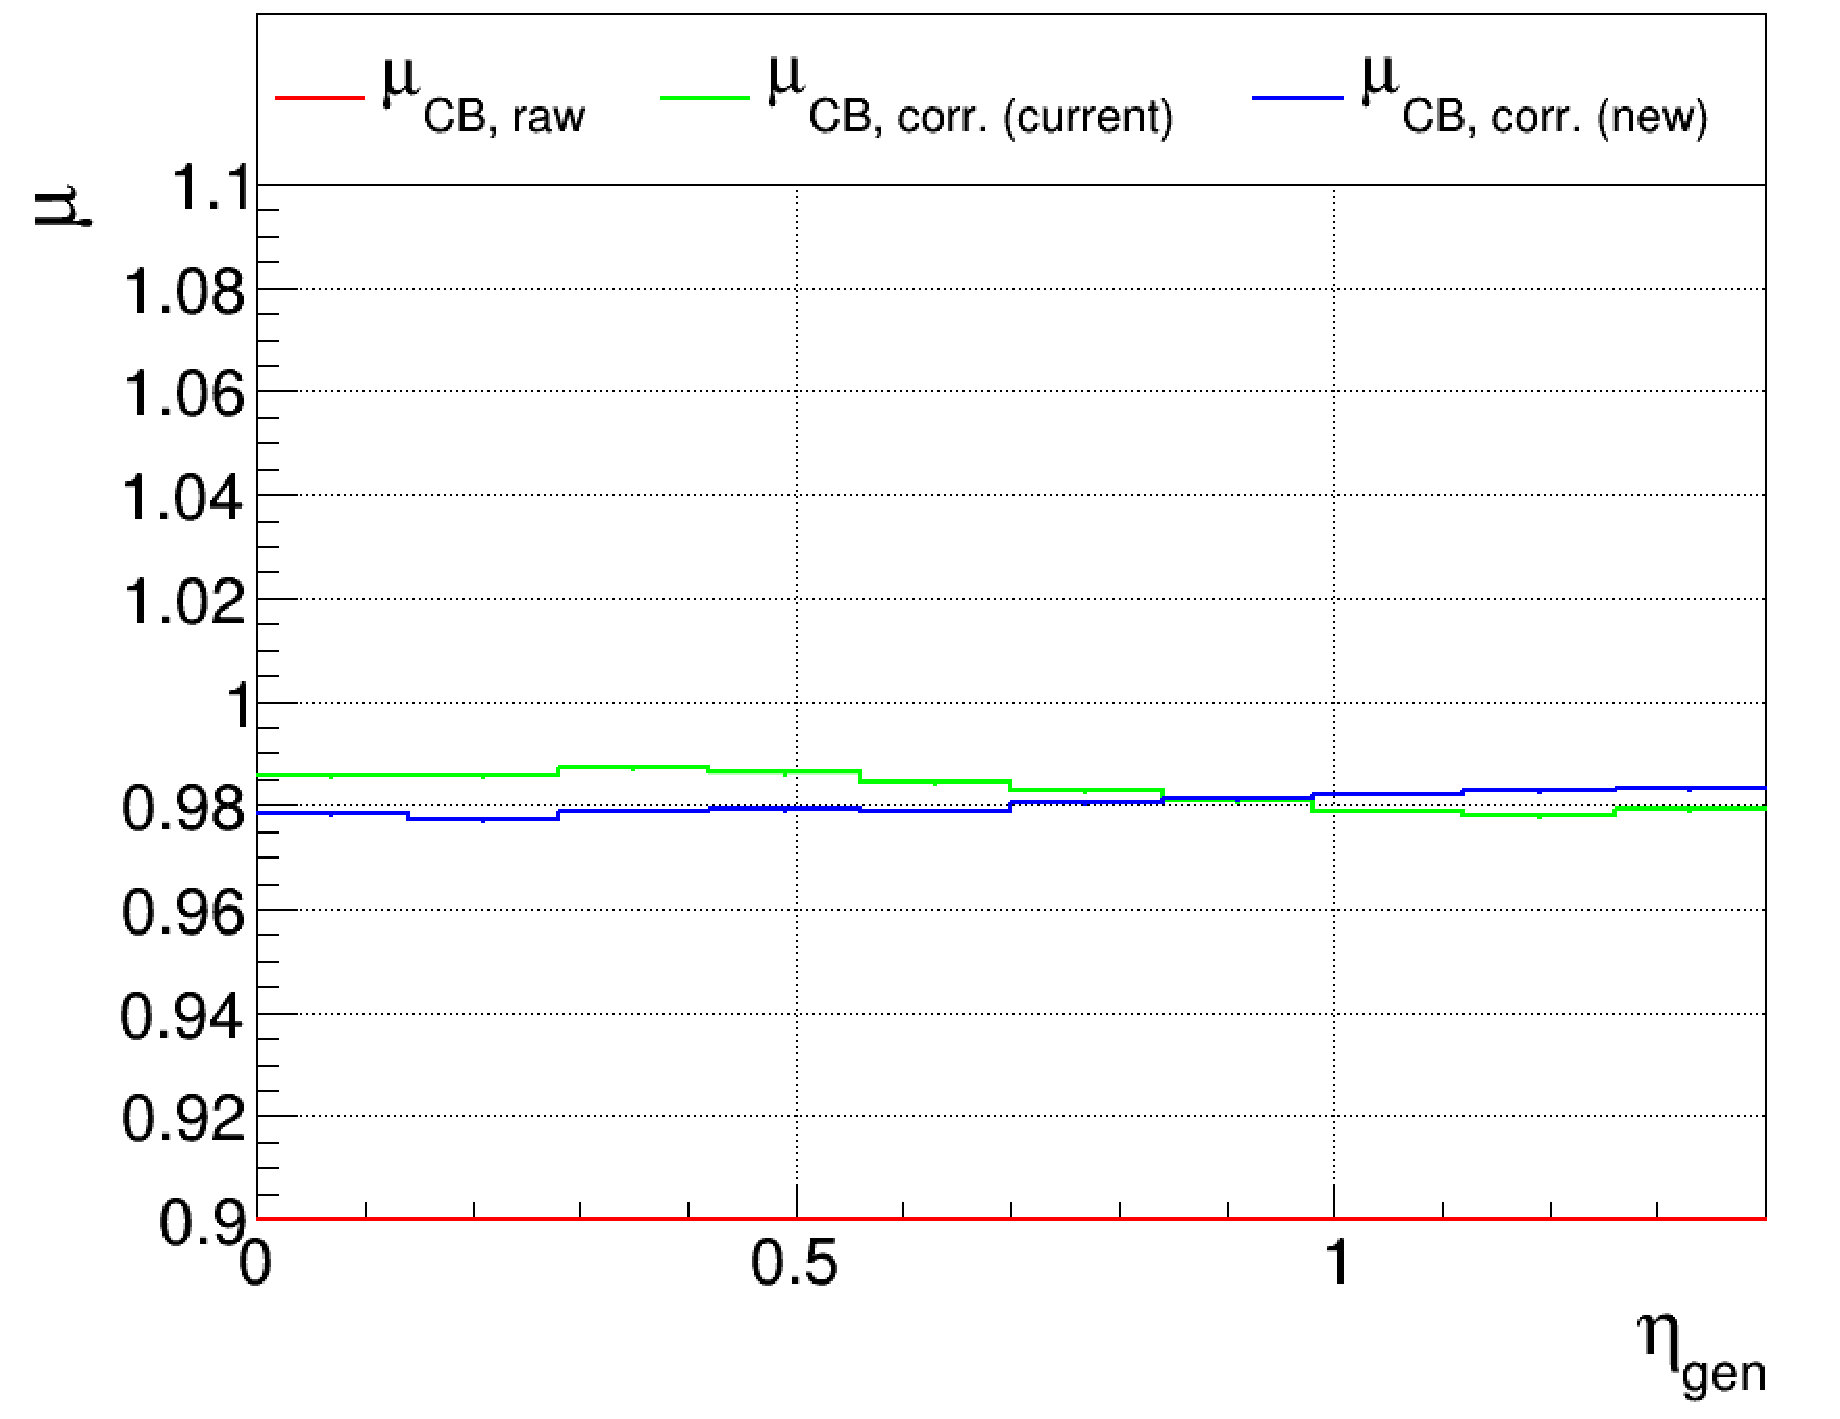
\includegraphics[width=0.495\textwidth]{./plots_pdf/ECAL_plots/plotsPU/EB/FULL/pdf/GENETA/EBFULL_GENETA_0005_0020_MuOverBins.pdf}
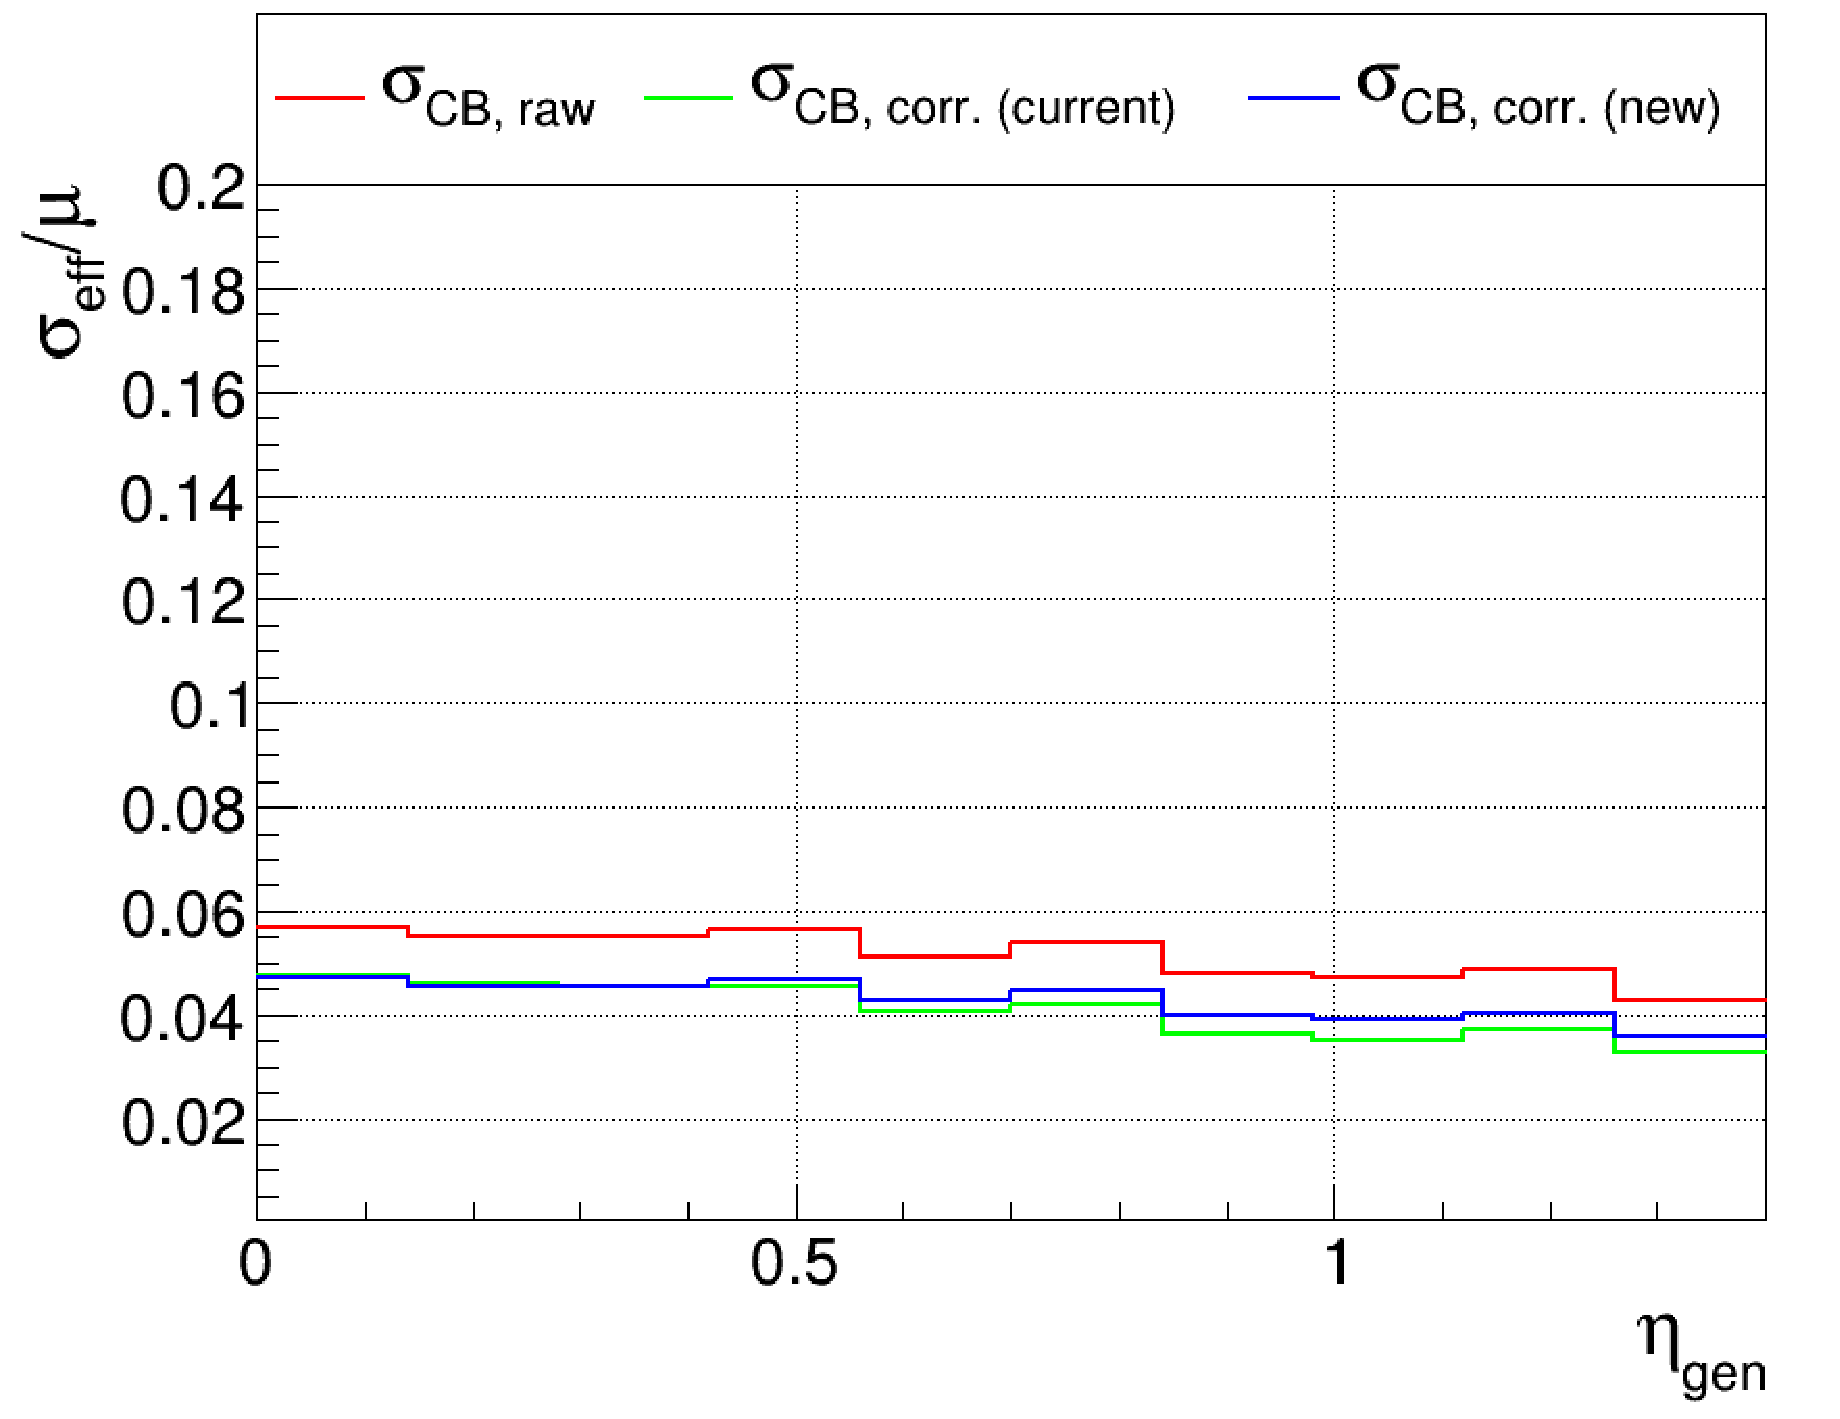
\includegraphics[width=0.495\textwidth]{./plots_pdf/ECAL_plots/plotsPU/EB/FULL/pdf/GENETA/EBFULL_GENETA_0005_0020_EffSigmaOverBins.pdf}
\caption{EB - Full Readout \pt 5--20\GeV.}
\end{figure}


\begin{figure}
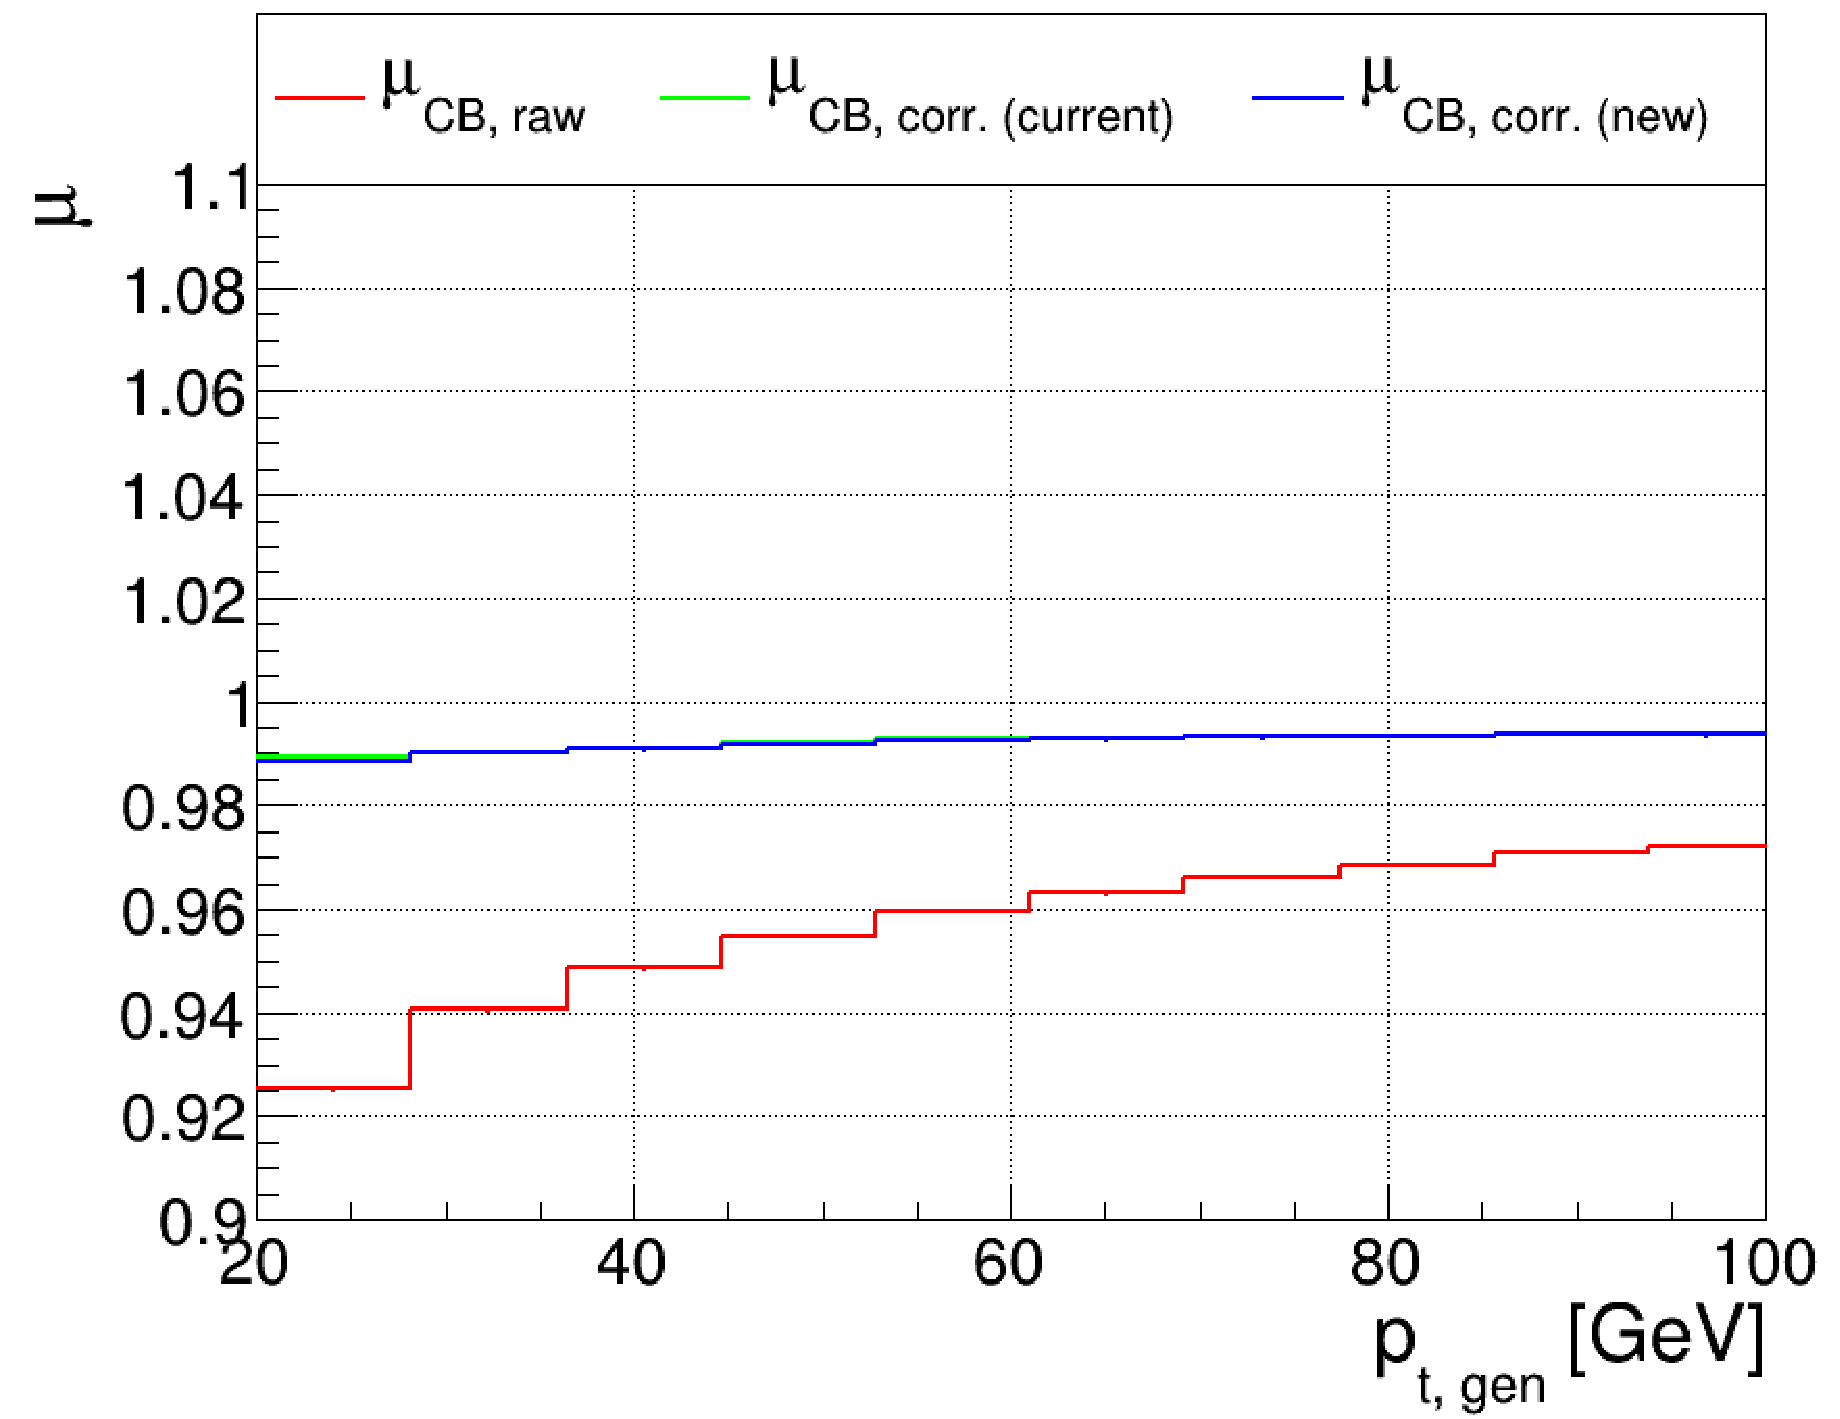
\includegraphics[width=0.495\textwidth]{./plots_pdf/ECAL_plots/plotsPU/EB/FULL/pdf/GENPT/EBFULL_GENPT_0020_0100_MuOverBins.pdf}
\includegraphics[width=0.495\textwidth]{./plots_pdf/ECAL_plots/plotsPU/EB/FULL/pdf/GENPT/EBFULL_GENPT_0020_0100_EffSigmaOverBins.pdf}
%\caption{EB - Full Readout pt 20-100}
%\end{figure}
%\begin{figure}
\includegraphics[width=0.495\textwidth]{./plots_pdf/ECAL_plots/plotsPU/EB/FULL/pdf/GENETA/EBFULL_GENETA_0020_0100_MuOverBins.pdf}
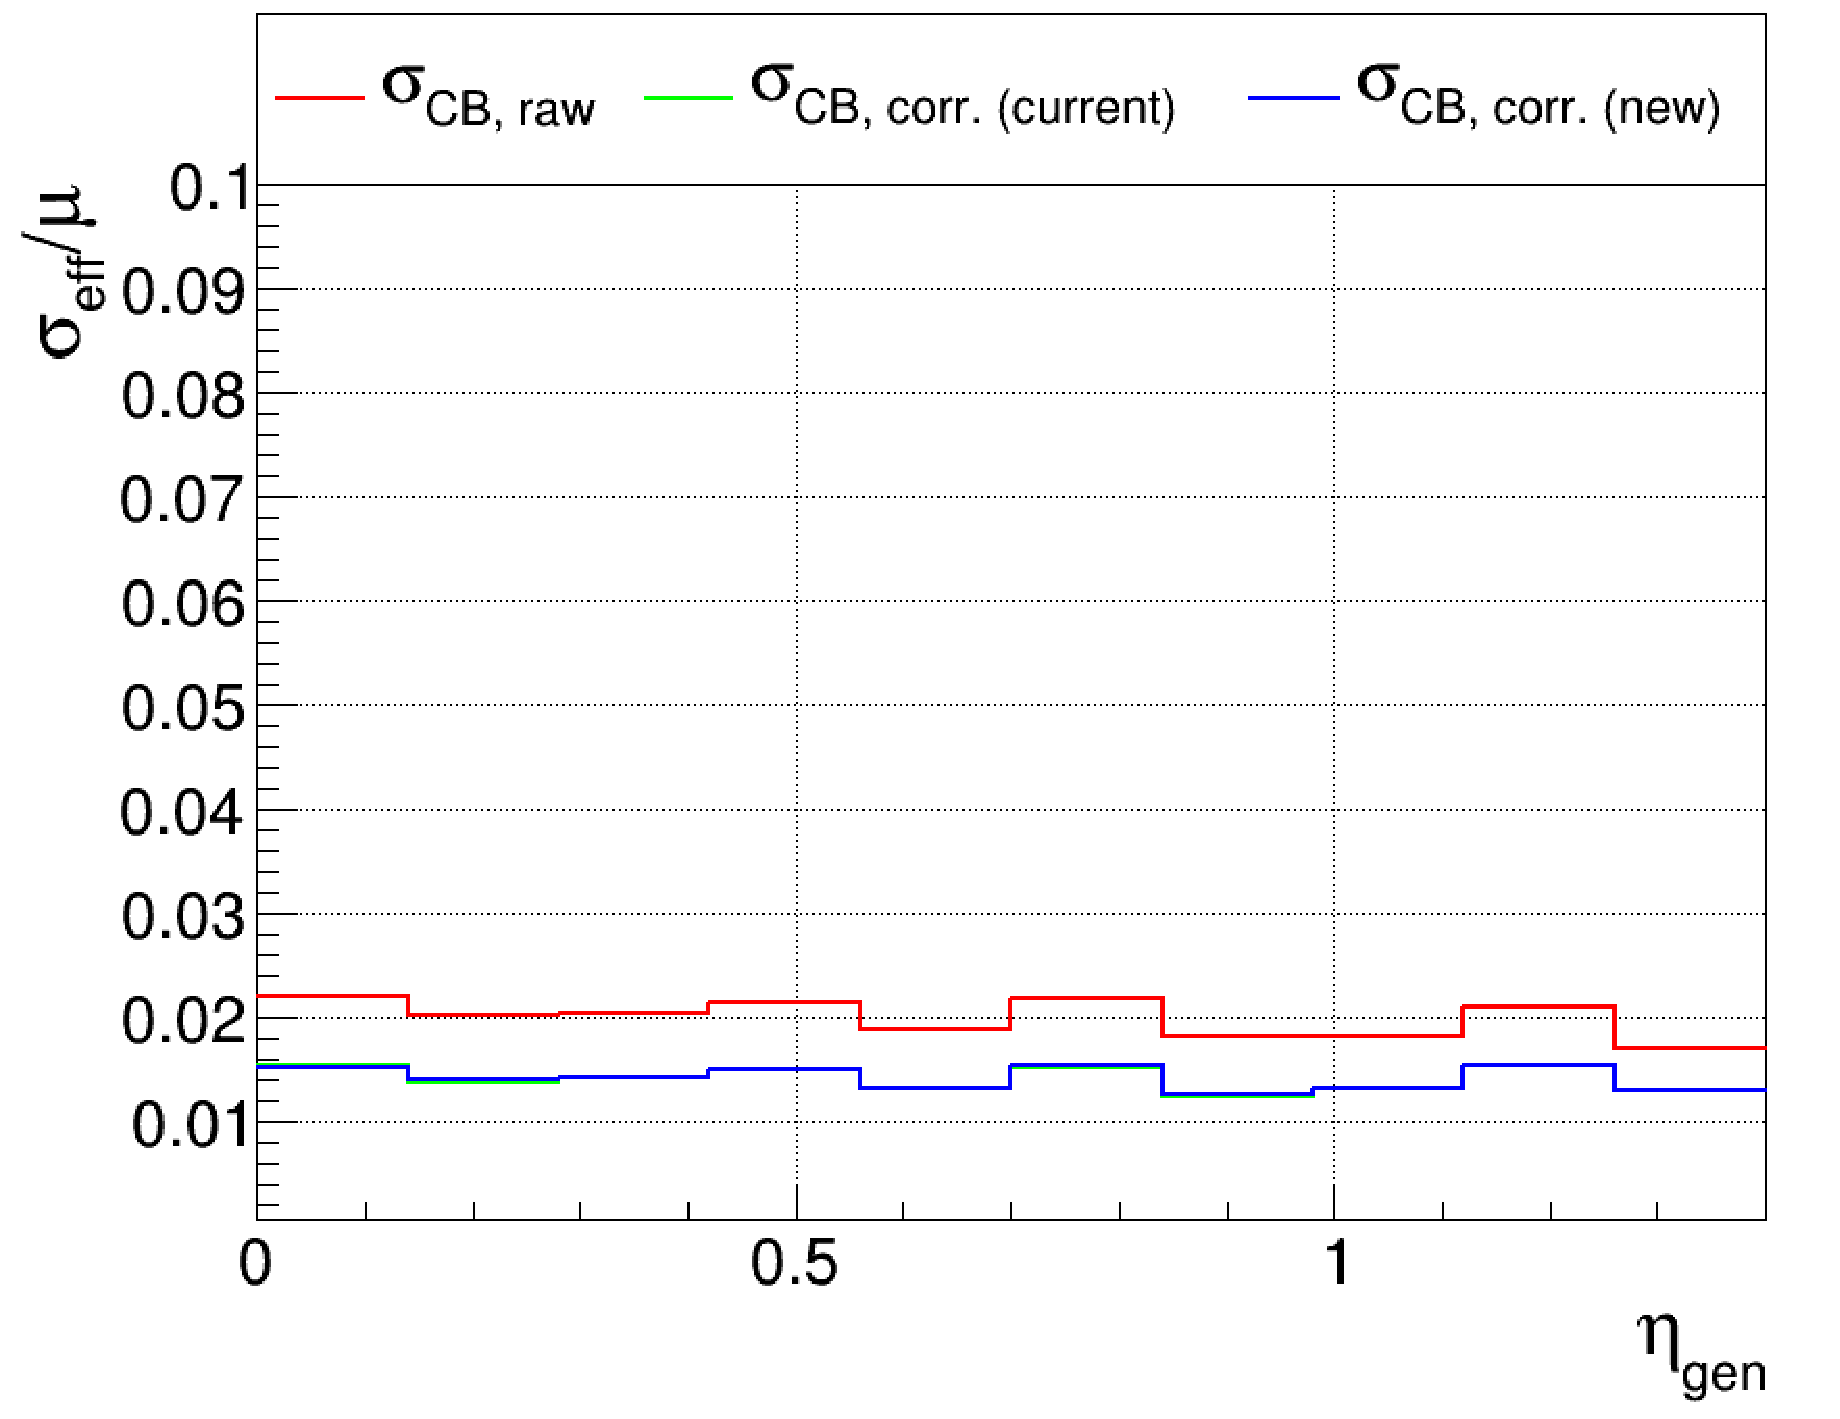
\includegraphics[width=0.495\textwidth]{./plots_pdf/ECAL_plots/plotsPU/EB/FULL/pdf/GENETA/EBFULL_GENETA_0020_0100_EffSigmaOverBins.pdf}
\caption{EB - Full Readout \pt 20--100\GeV.}
\end{figure}

\begin{figure}
\includegraphics[width=0.495\textwidth]{./plots_pdf/ECAL_plots/plotsPU/EB/FULL/pdf/GENPT/EBFULL_GENPT_0100_0300_MuOverBins.pdf}
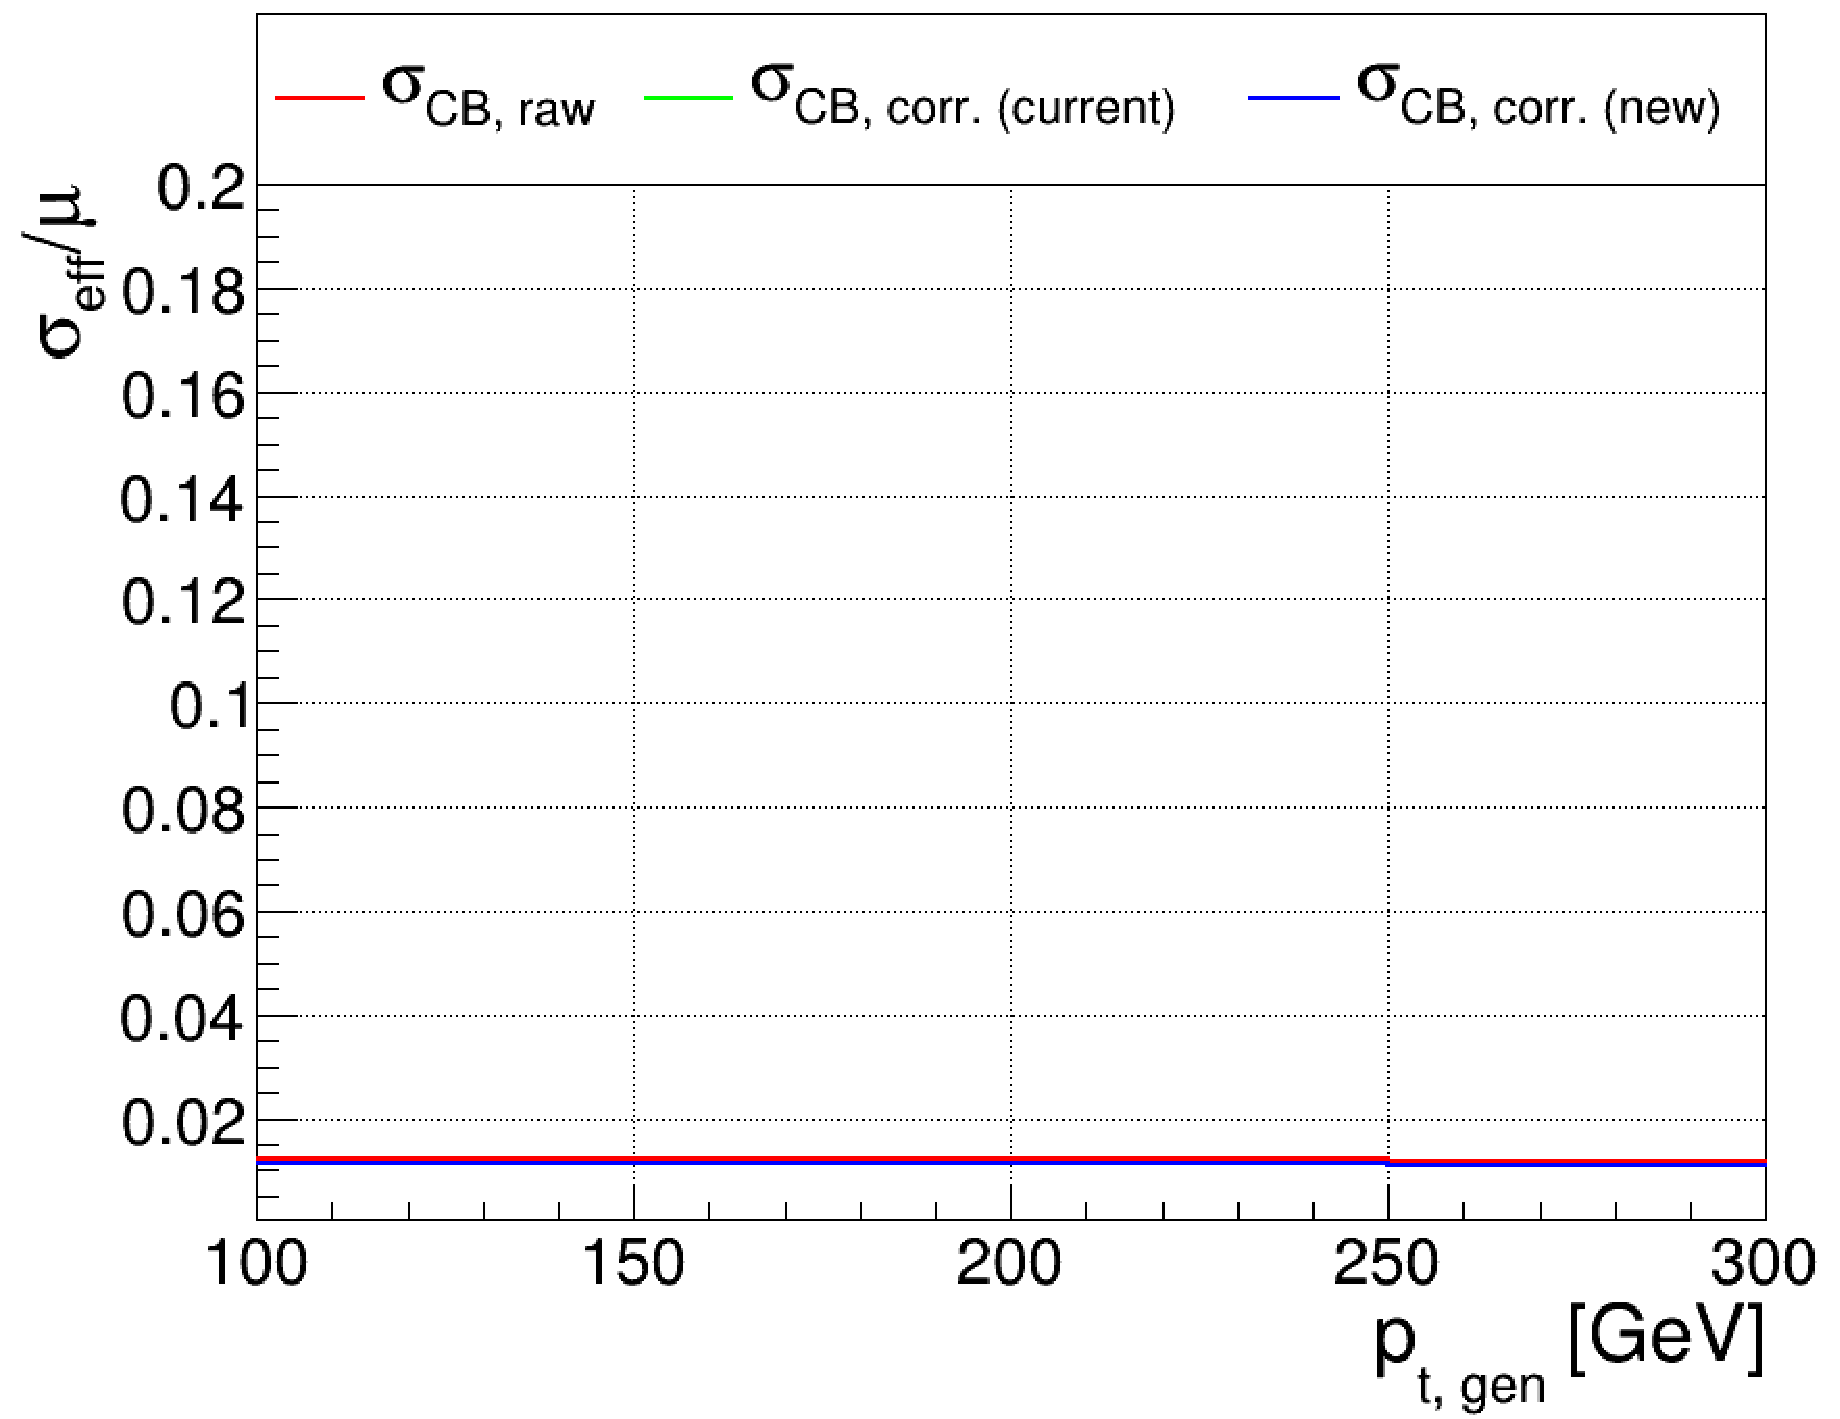
\includegraphics[width=0.495\textwidth]{./plots_pdf/ECAL_plots/plotsPU/EB/FULL/pdf/GENPT/EBFULL_GENPT_0100_0300_EffSigmaOverBins.pdf}
%\caption{EB - Full Readout pt 100-300}
%\end{figure}
%\begin{figure}
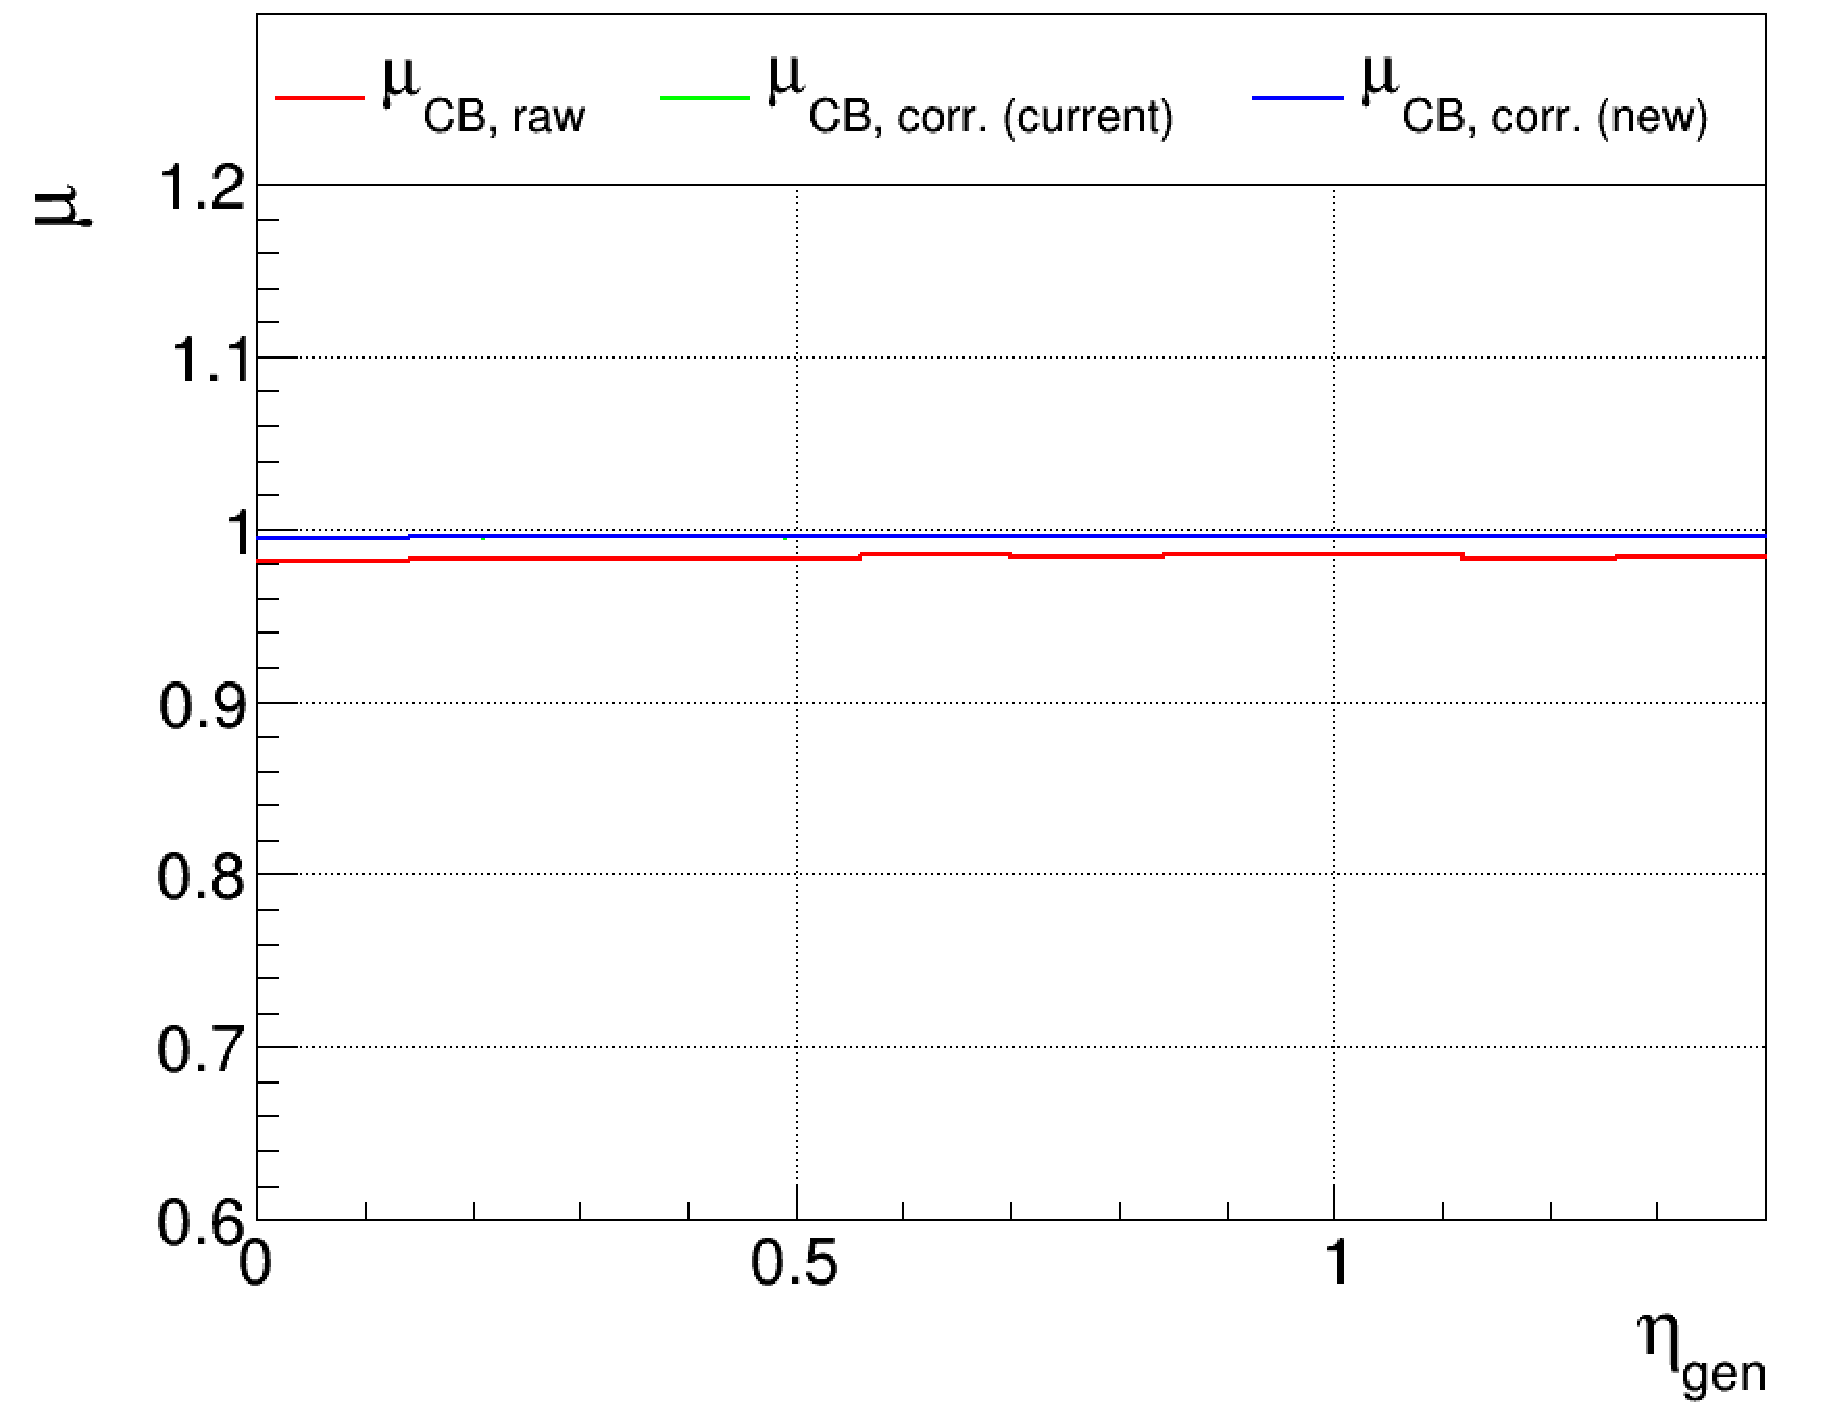
\includegraphics[width=0.495\textwidth]{./plots_pdf/ECAL_plots/plotsPU/EB/FULL/pdf/GENETA/EBFULL_GENETA_0100_0300_MuOverBins.pdf}
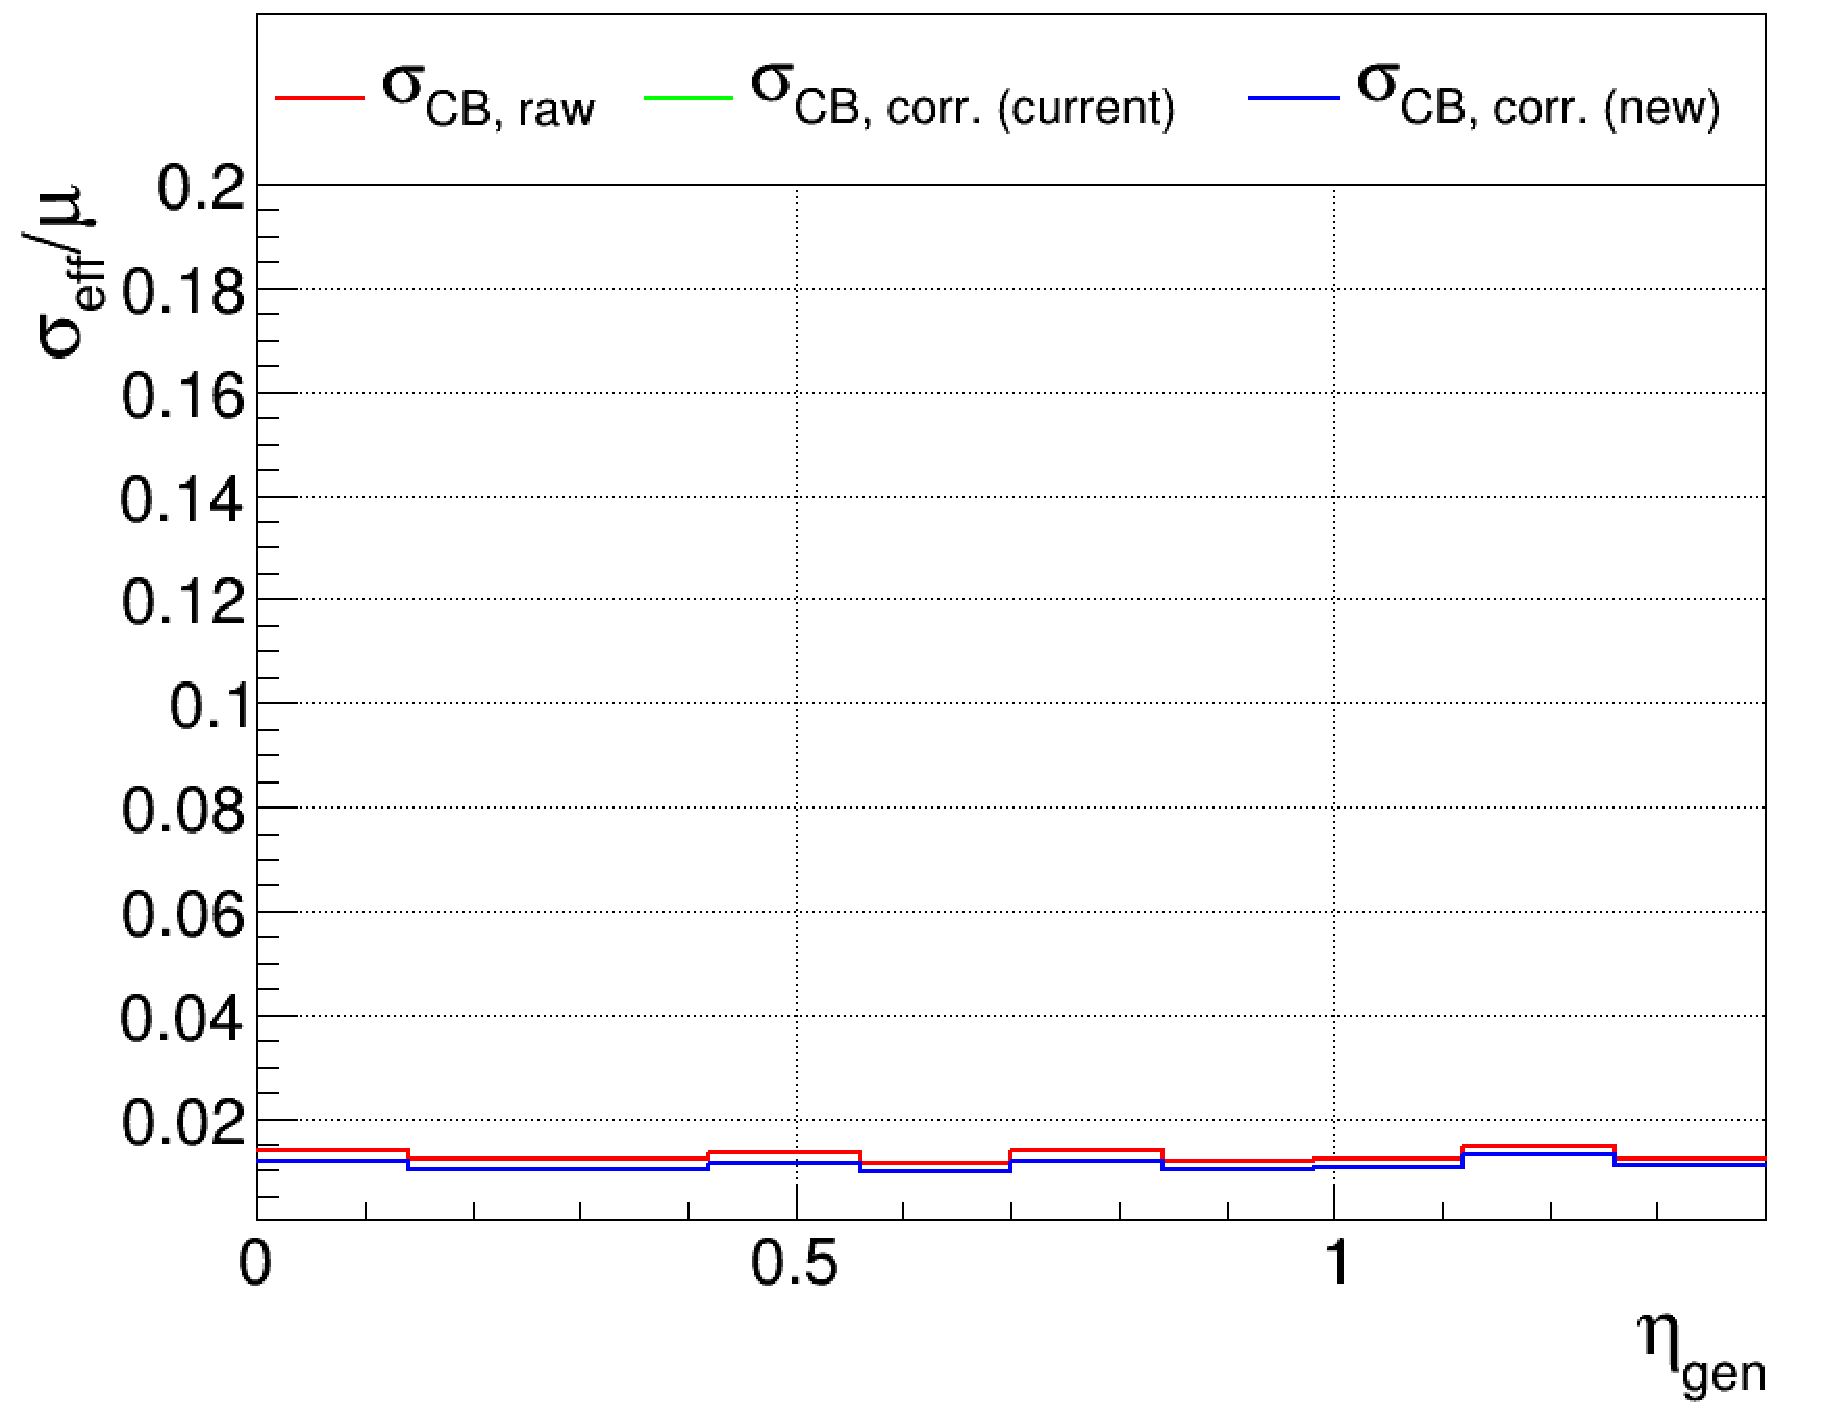
\includegraphics[width=0.495\textwidth]{./plots_pdf/ECAL_plots/plotsPU/EB/FULL/pdf/GENETA/EBFULL_GENETA_0100_0300_EffSigmaOverBins.pdf}
\caption{EB - Full Readout \pt 100-300\GeV}
\end{figure}





\begin{figure}
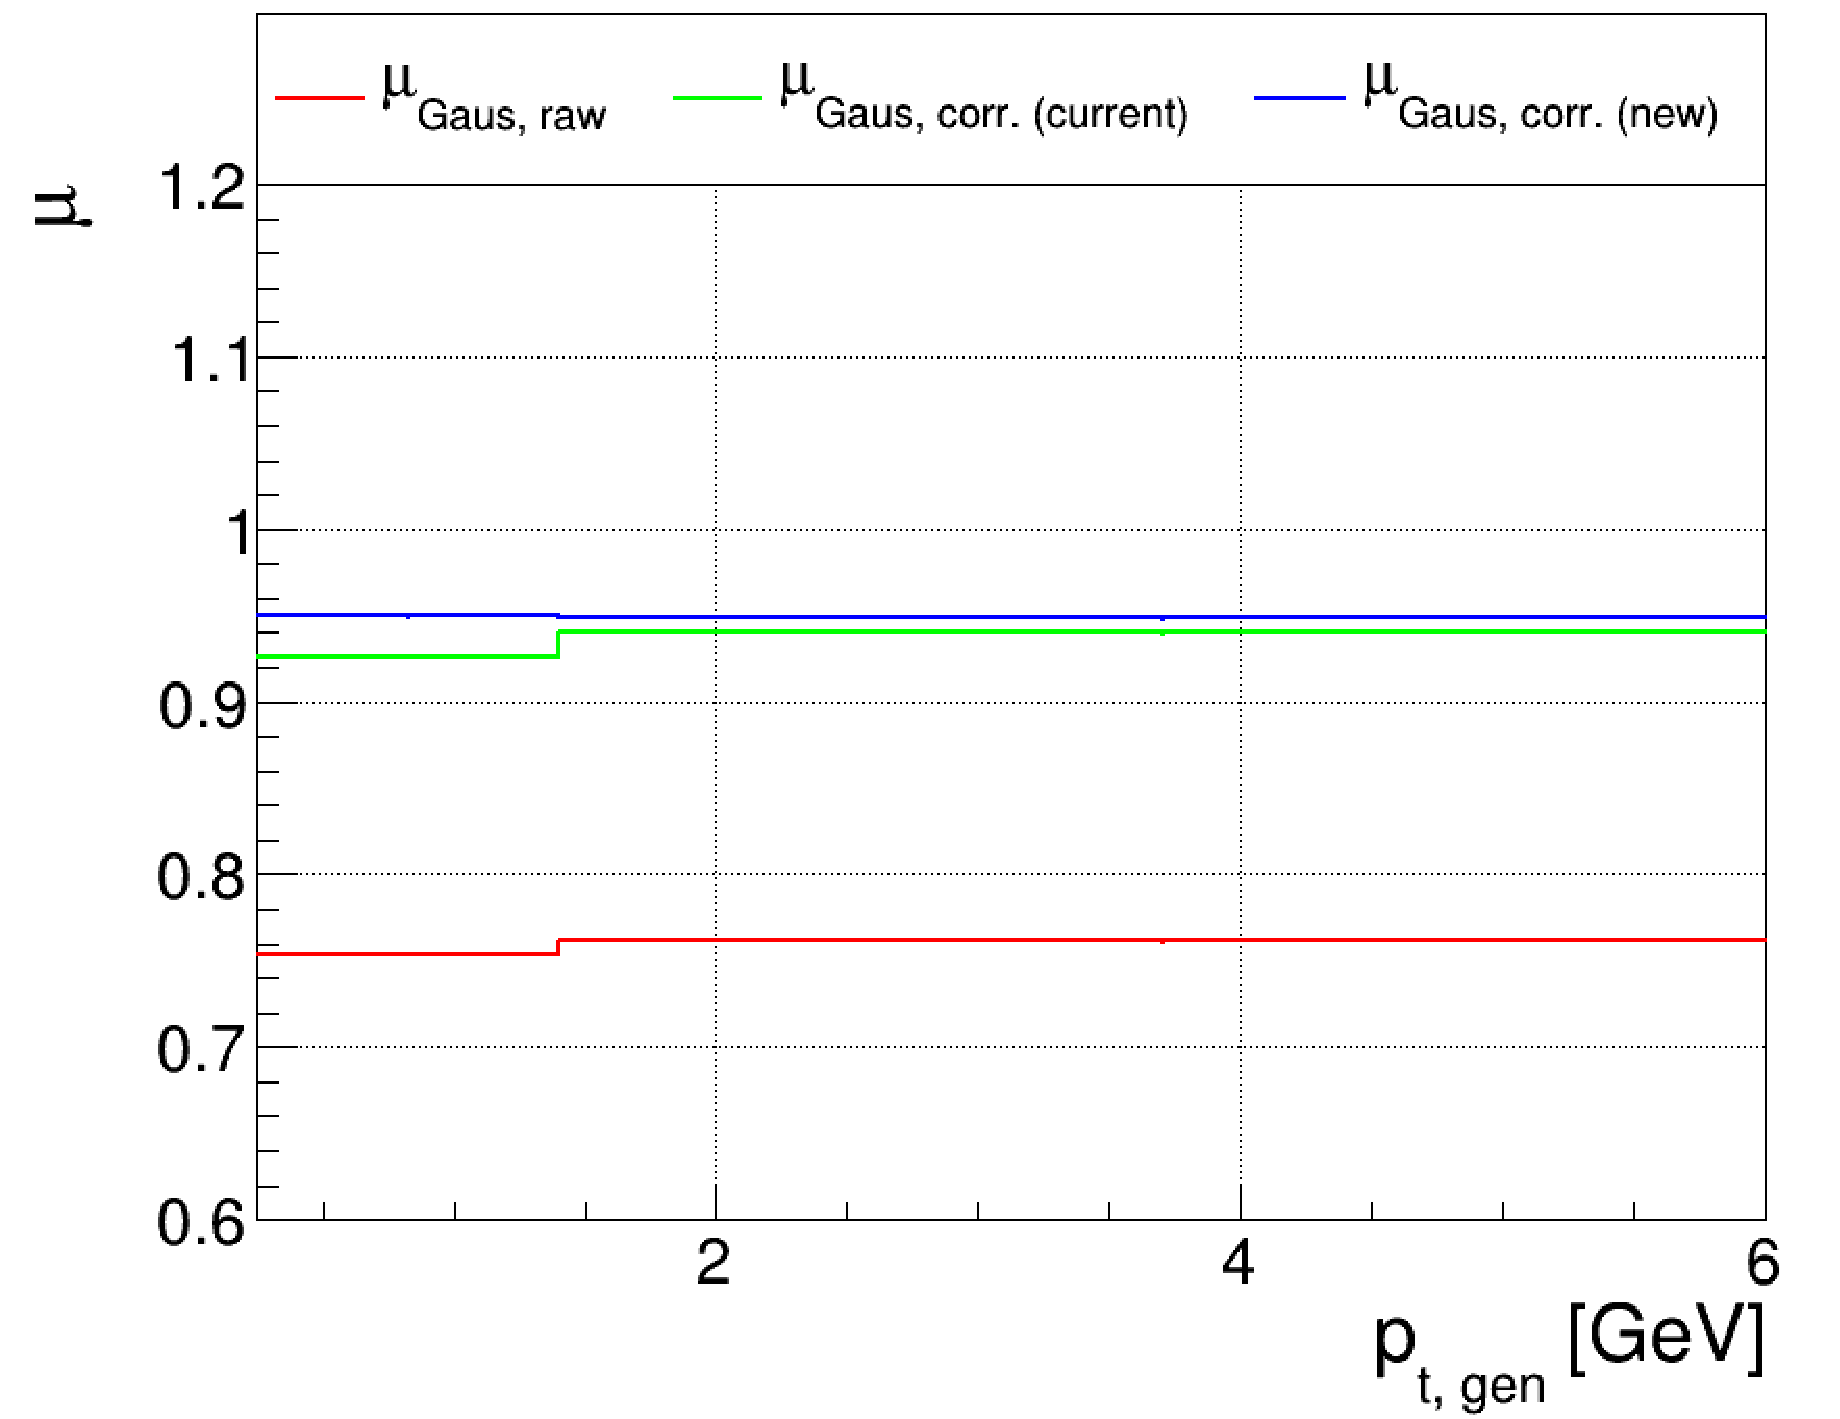
\includegraphics[width=0.495\textwidth]{./plots_pdf/ECAL_plots/plotsPU/EB/ZS/pdf/GENPT/EBZS_GENPT_0000_0006_MuOverBins.pdf}
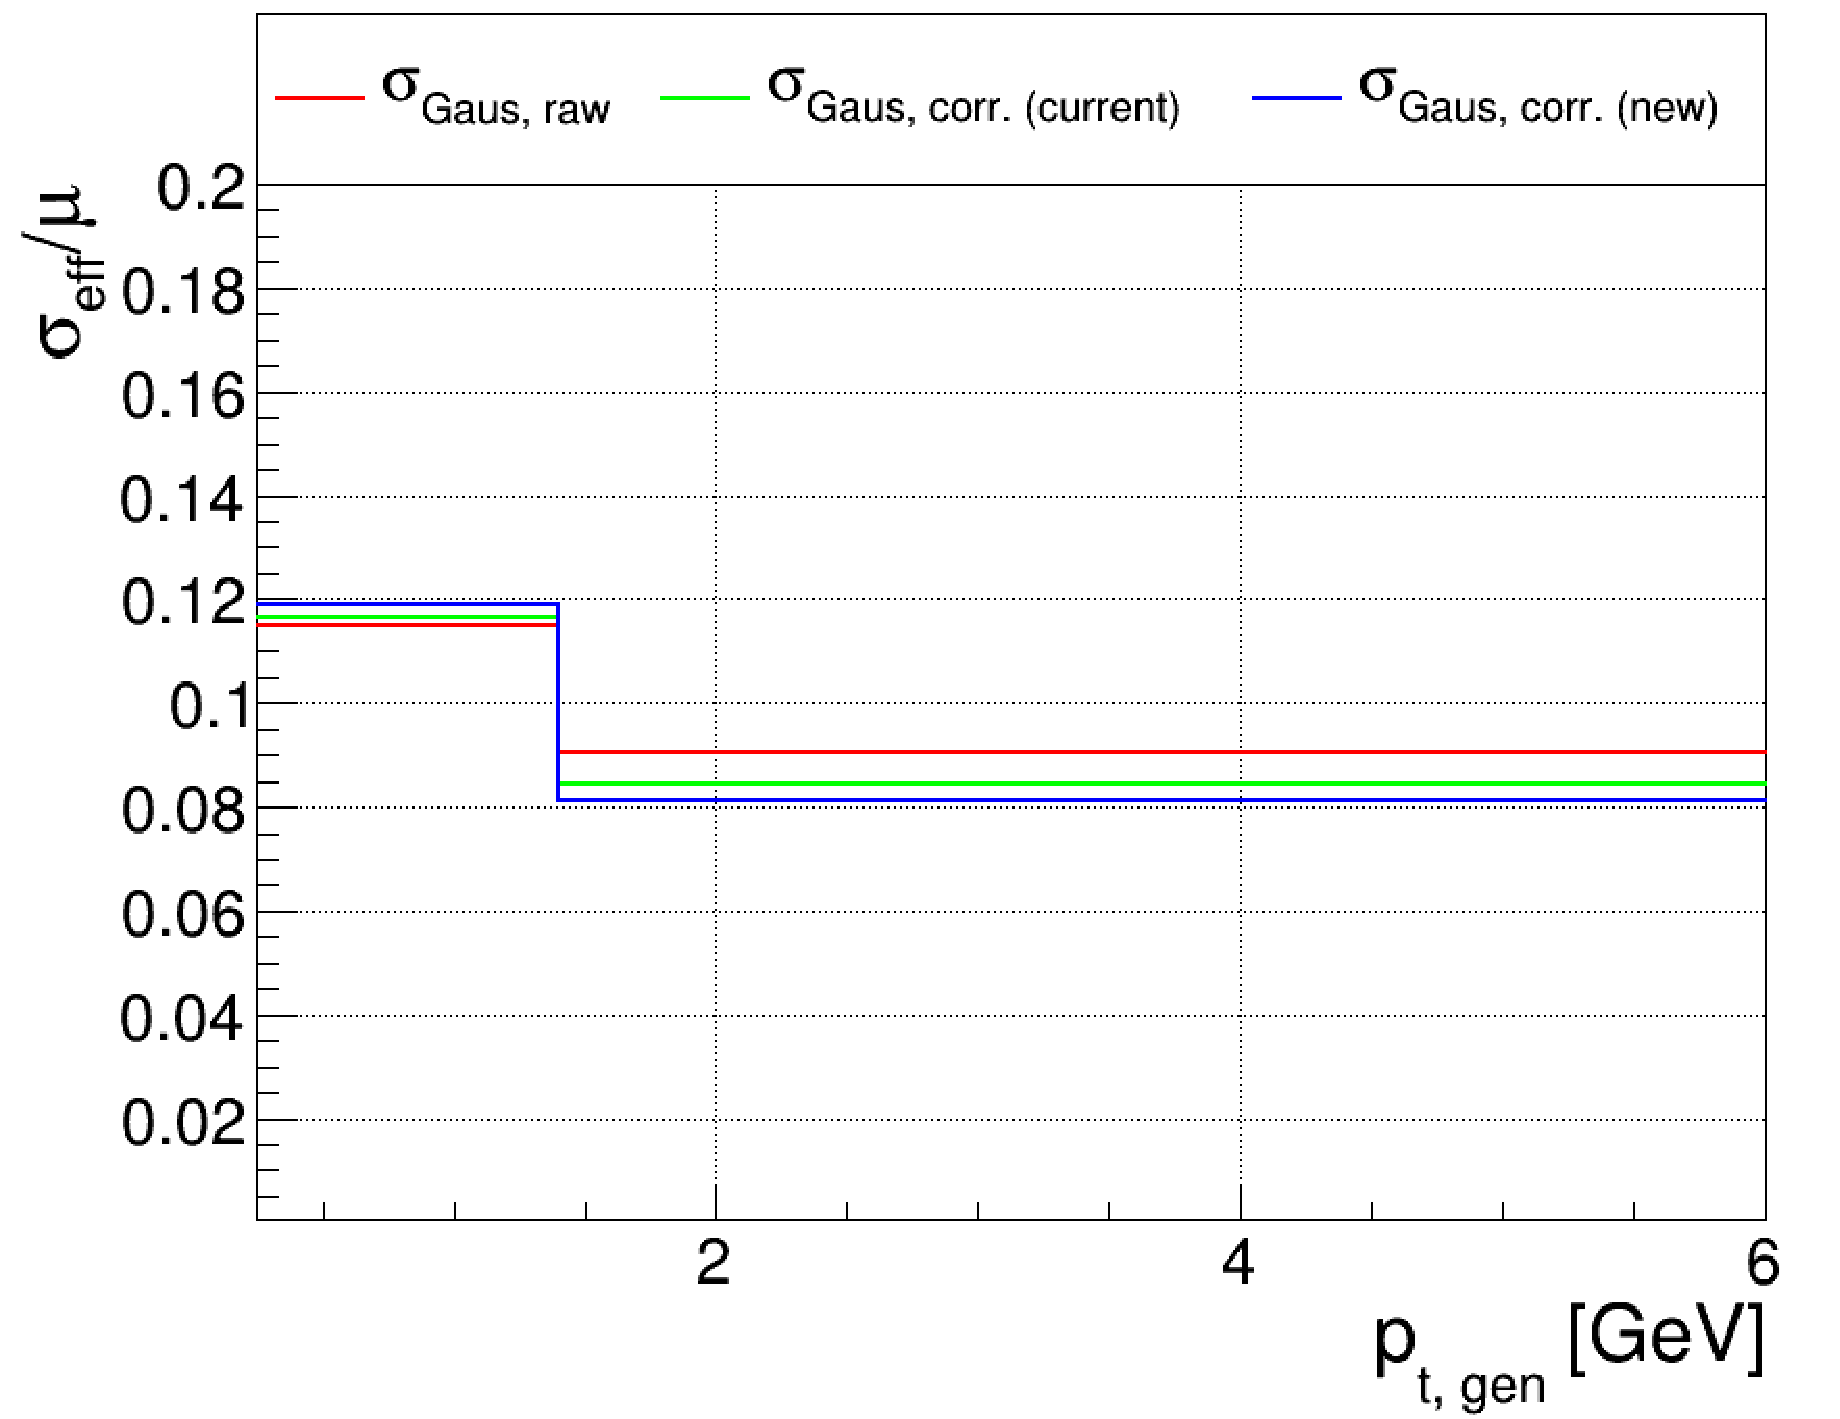
\includegraphics[width=0.495\textwidth]{./plots_pdf/ECAL_plots/plotsPU/EB/ZS/pdf/GENPT/EBZS_GENPT_0000_0006_EffSigmaOverBins.pdf}

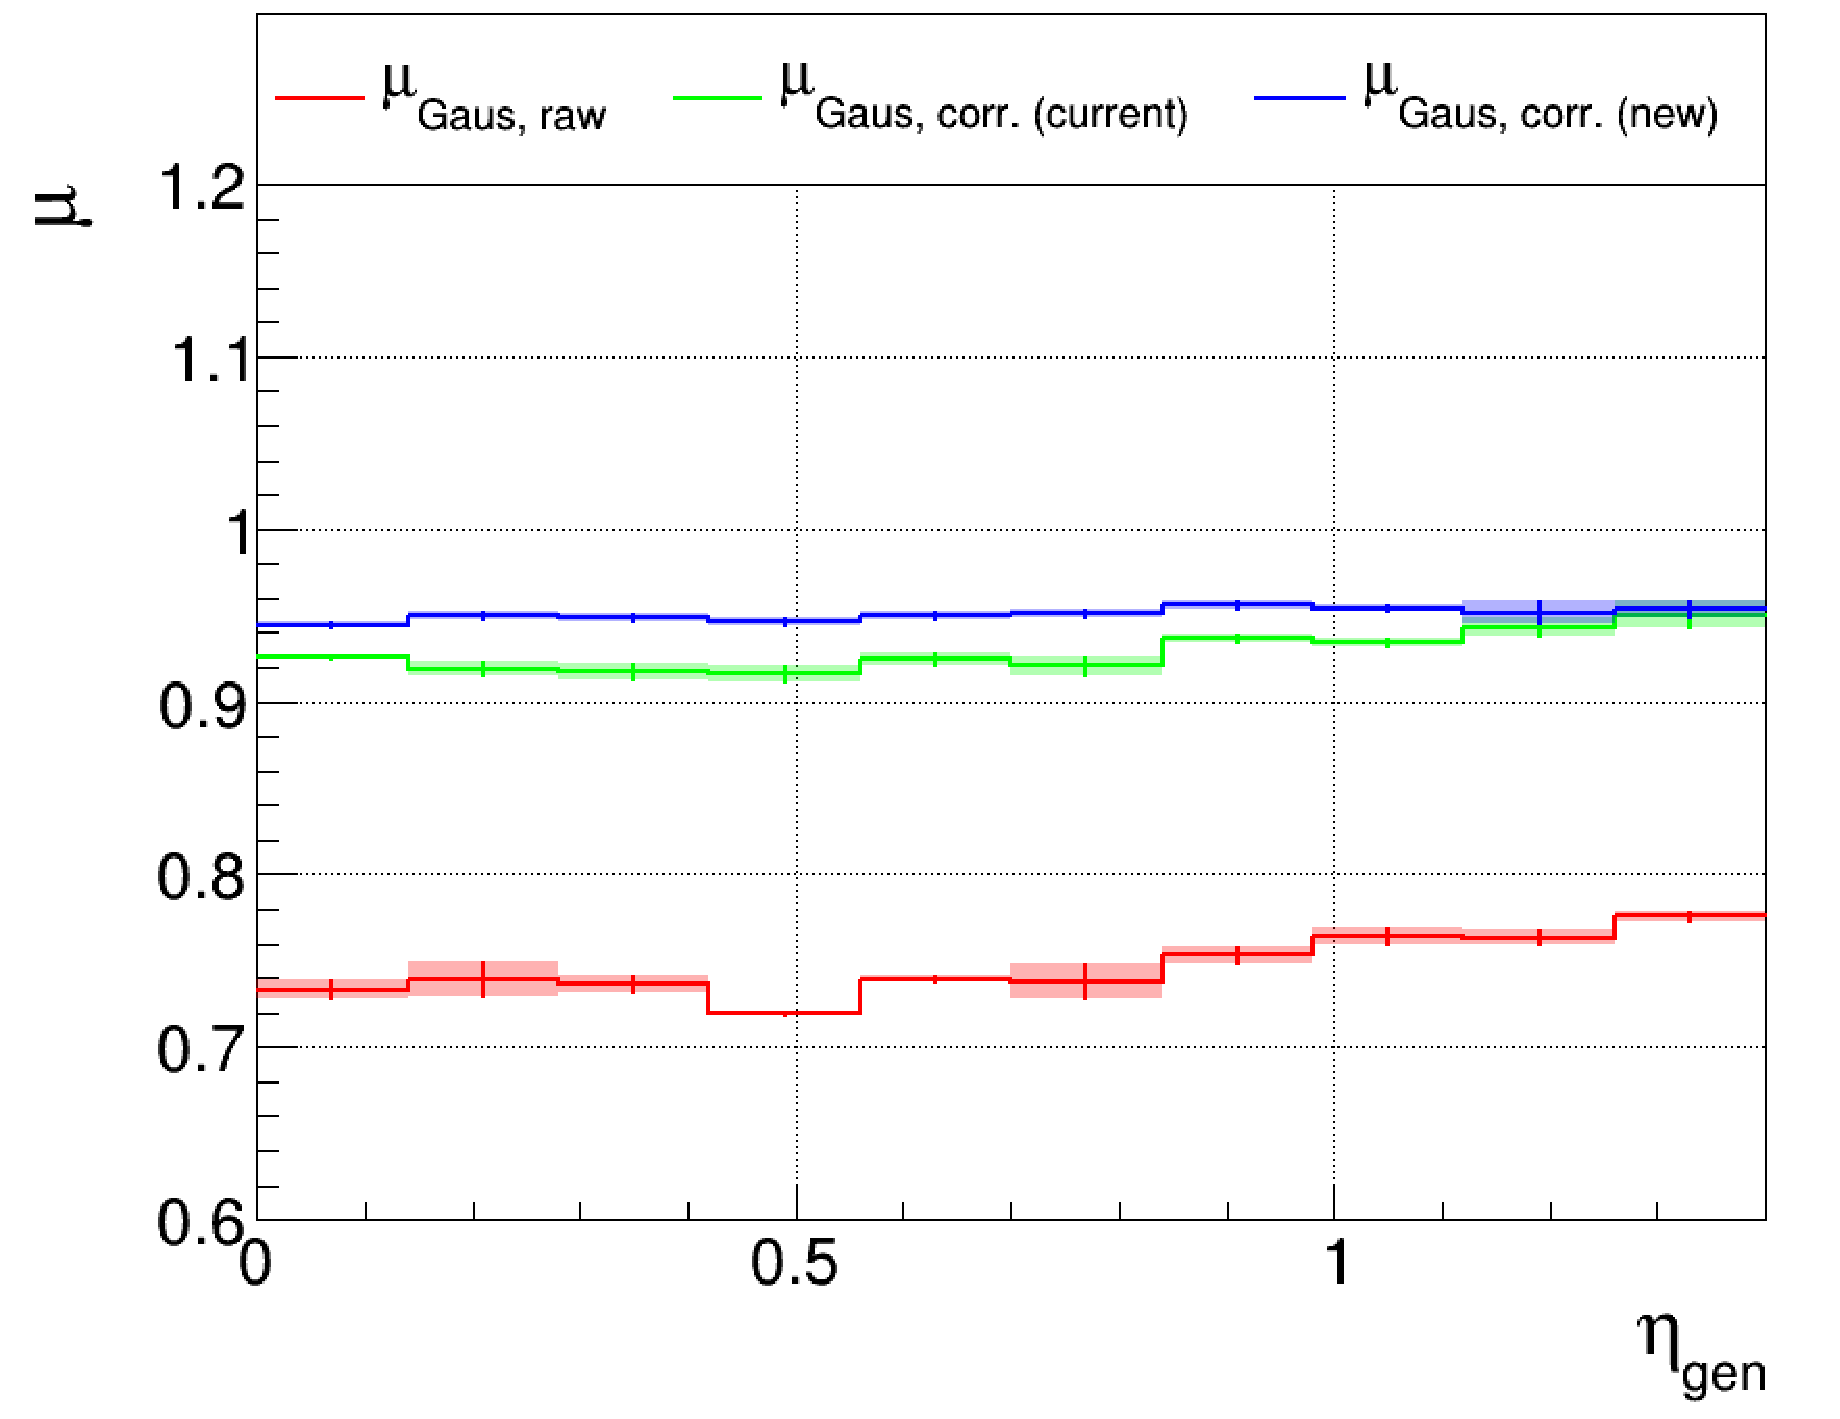
\includegraphics[width=0.495\textwidth]{./plots_pdf/ECAL_plots/plotsPU/EB/ZS/pdf/GENETA/EBZS_GENETA_0000_0006_MuOverBins.pdf}
\includegraphics[width=0.495\textwidth]{./plots_pdf/ECAL_plots/plotsPU/EB/ZS/pdf/GENETA/EBZS_GENETA_0000_0006_EffSigmaOverBins.pdf}
\caption[$\mu$ ($\sigma_\mathrm{eff}$) vs \pt of PF ECAL cluster - EB ZS readout PU  senario]{Mean response (resolution) defined by Raw PF ECAL clusters (red), the calibration derived earlier in Ru\
n3 based on 126X (green), and the new correction from 2024 simulation sample based on 133X (blue). \pt 0--6\GeV PU EB ZS readout PU senario.}
\label{fig:PU_EBZS}
\end{figure}

%% %\begin{figure}
%% \includegraphics[width=0.495\textwidth]{./plots_pdf/ECAL_plots/plotsPU/EB/ZS/pdf/GENPT/EBZS_GENPT_0006_0025_MuOverBins.pdf}
%% 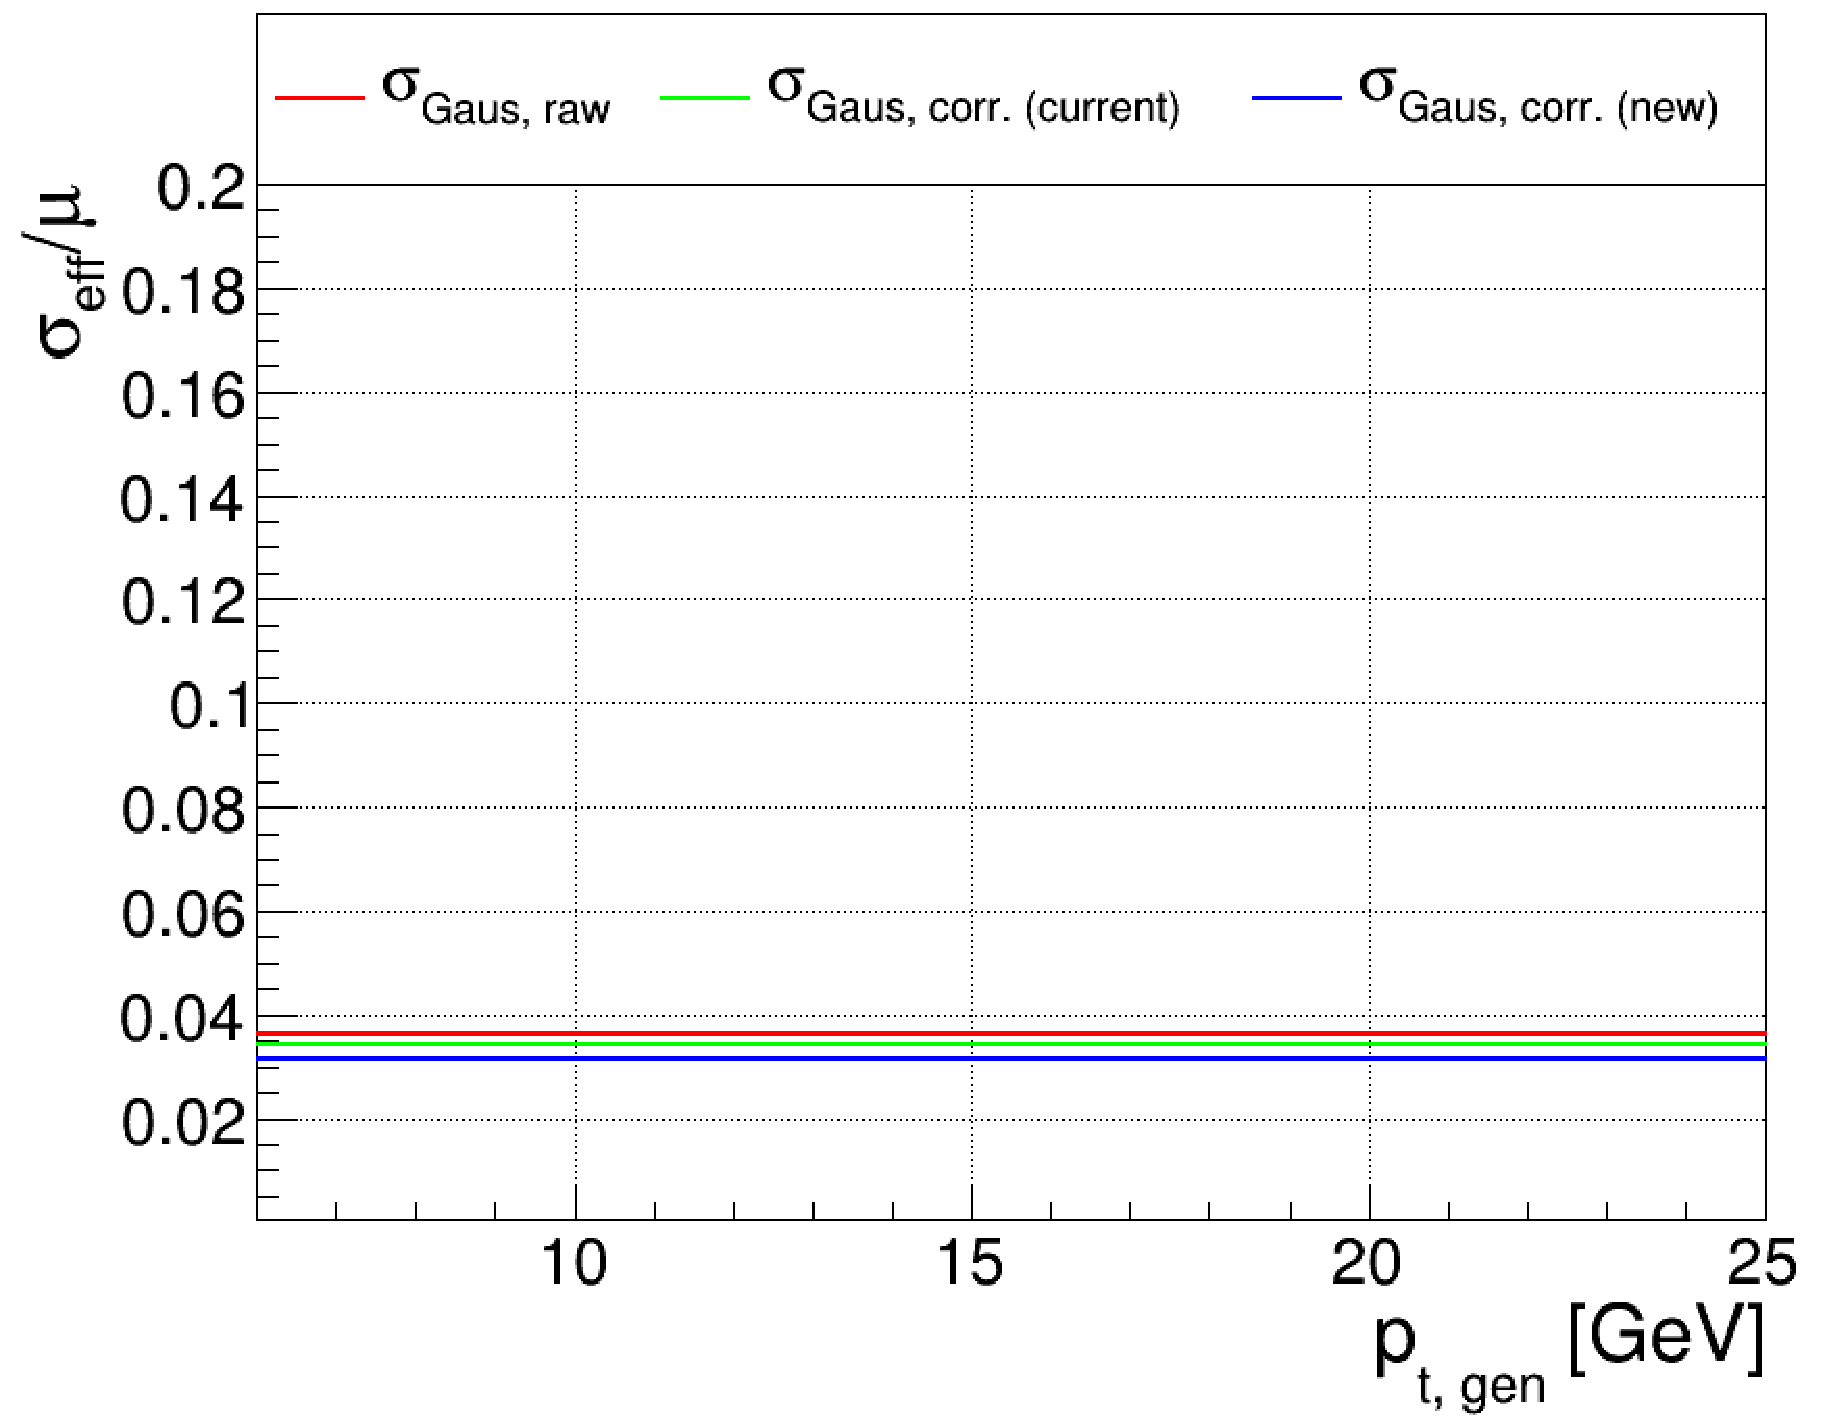
\includegraphics[width=0.495\textwidth]{./plots_pdf/ECAL_plots/plotsPU/EB/ZS/pdf/GENPT/EBZS_GENPT_0006_0025_EffSigmaOverBins.pdf}
%% %\caption{EB - ZS Readout pt 6-25}
%% %\end{figure}
%% %\begin{figure}
%% 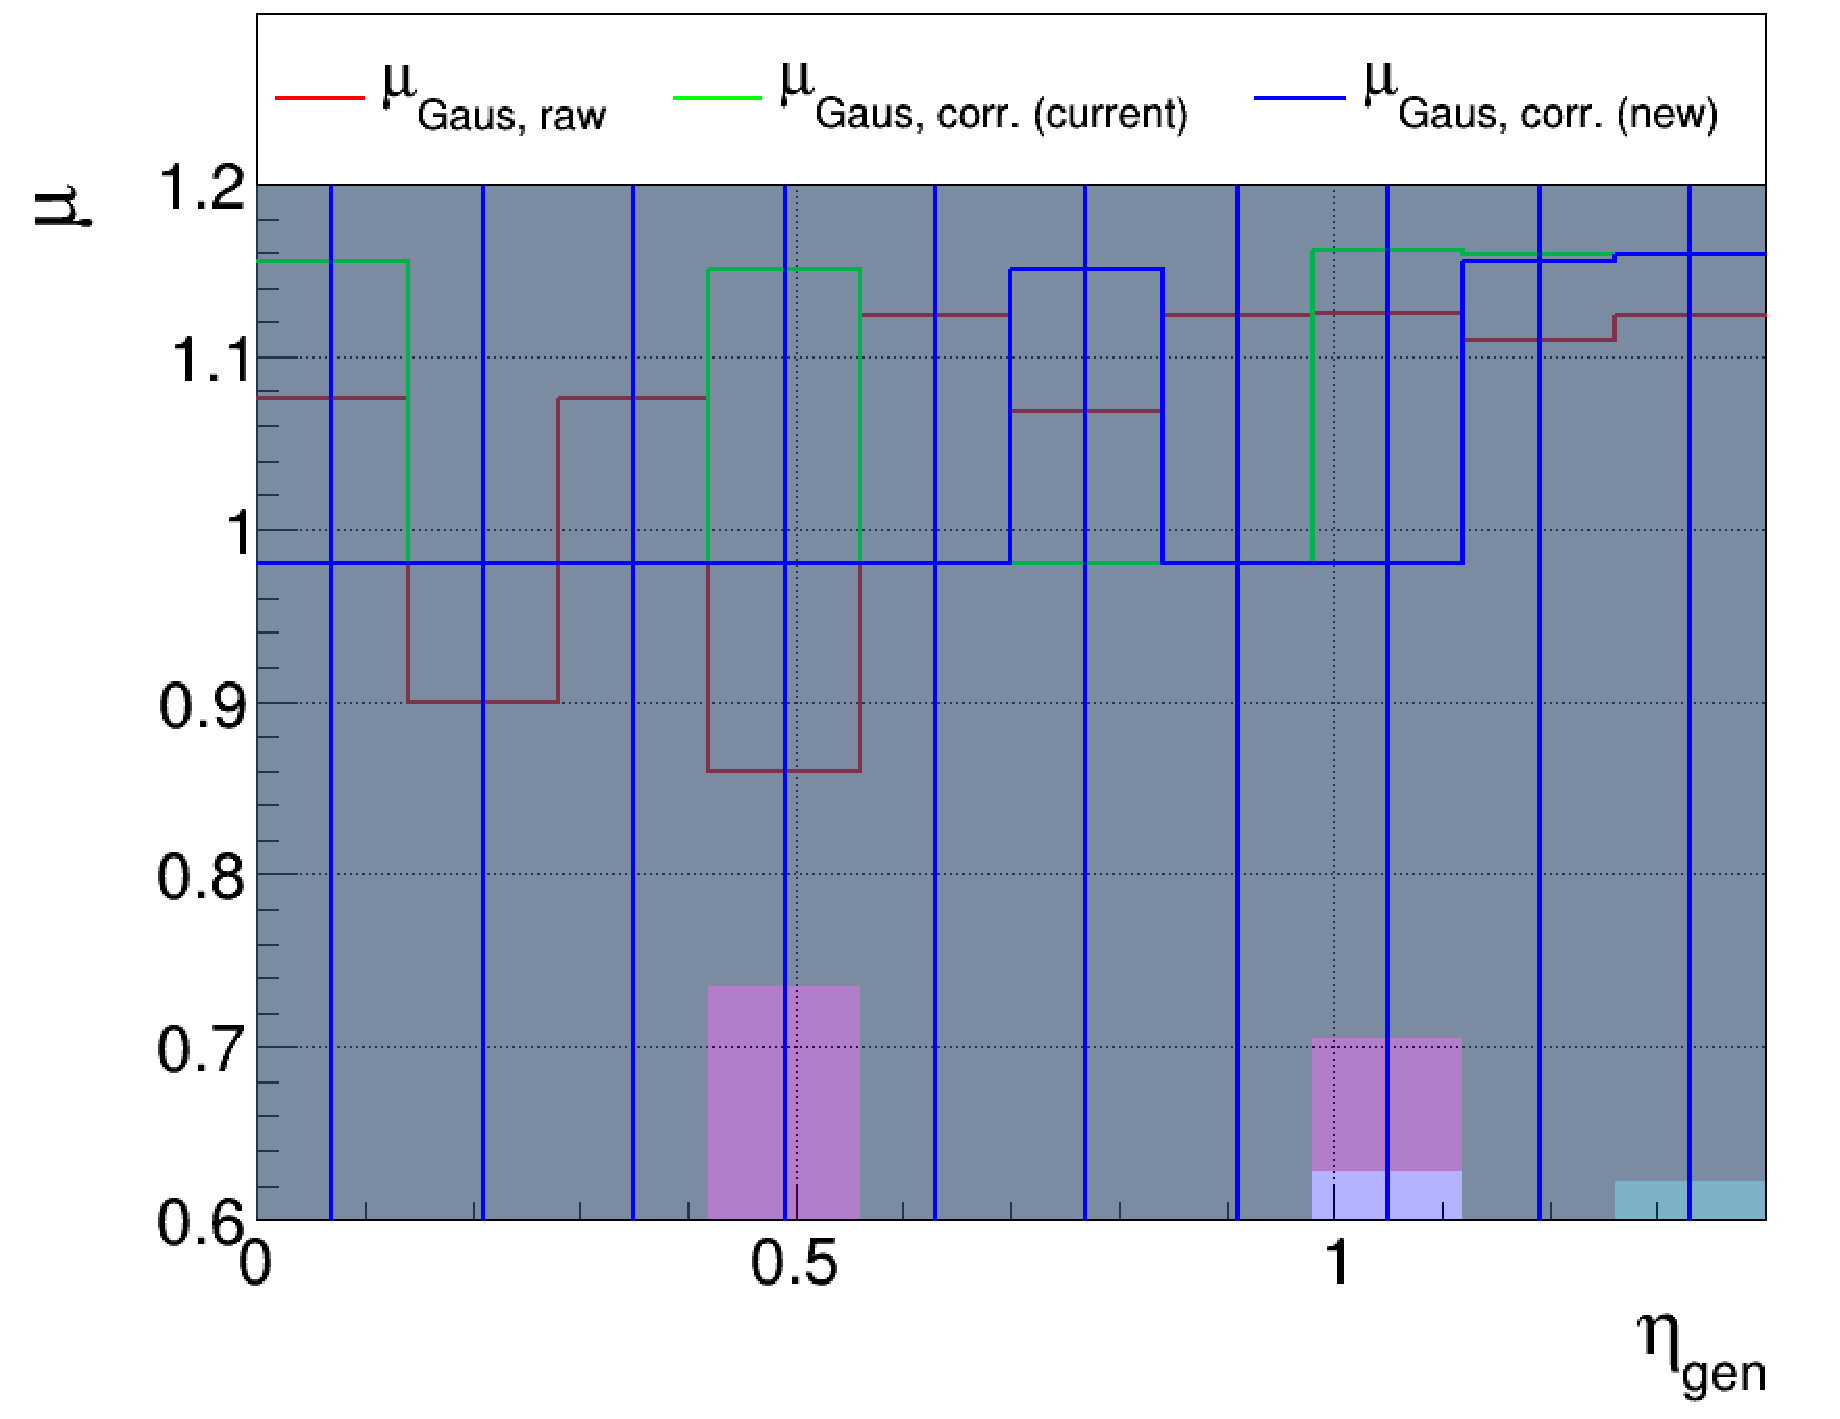
\includegraphics[width=0.495\textwidth]{./plots_pdf/ECAL_plots/plotsPU/EB/ZS/pdf/GENETA/EBZS_GENETA_0006_0025_MuOverBins.pdf}
%% 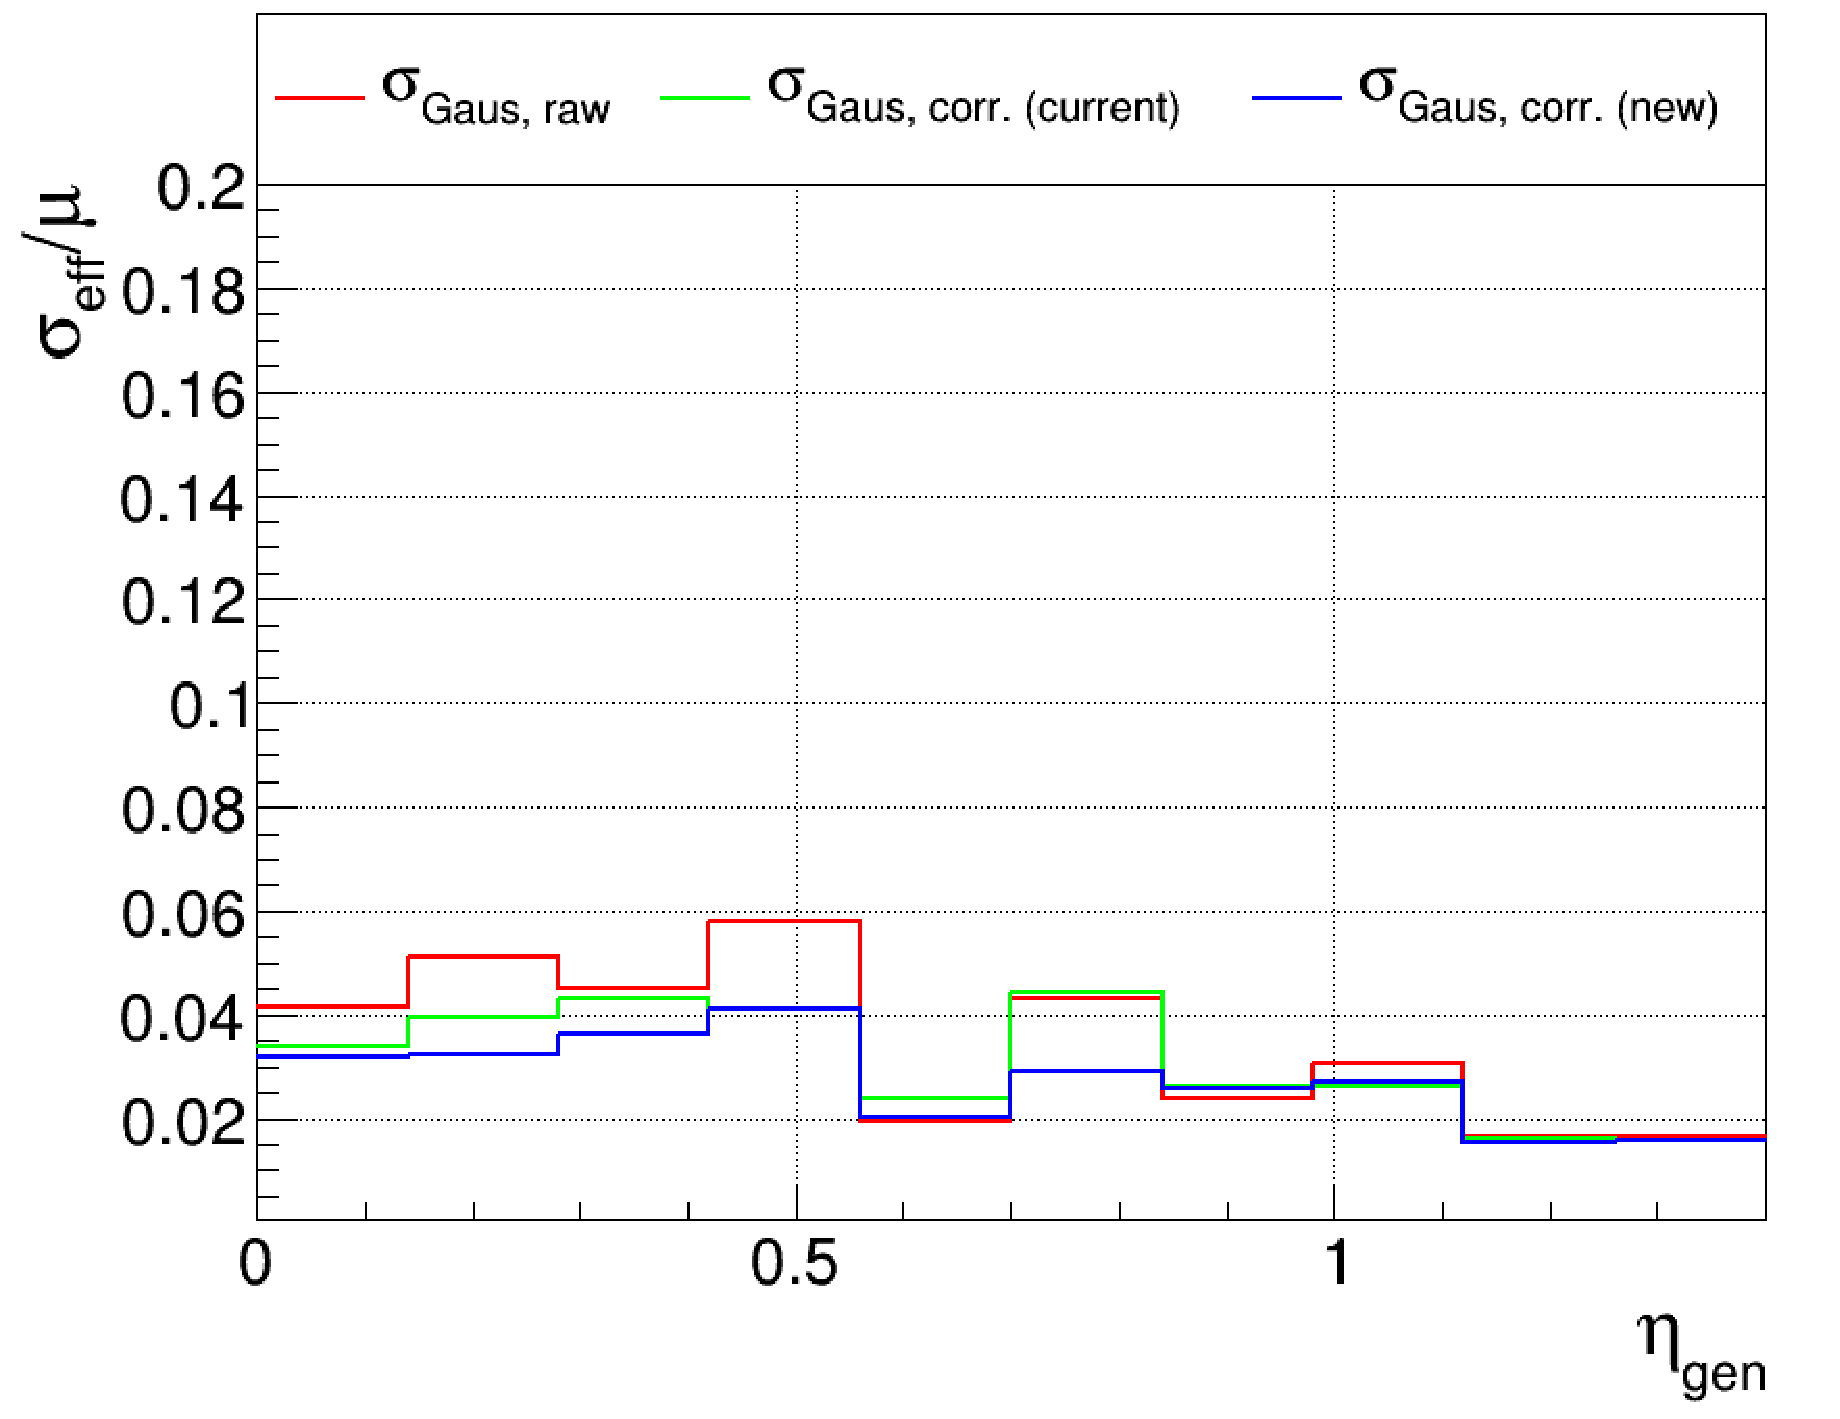
\includegraphics[width=0.495\textwidth]{./plots_pdf/ECAL_plots/plotsPU/EB/ZS/pdf/GENETA/EBZS_GENETA_0006_0025_EffSigmaOverBins.pdf}
%% \caption{EB - ZS Readout \pt 6-25}
%% \end{figure}







\begin{figure}
  %5-20 pt 
\includegraphics[width=0.335\textwidth]{./plots_pdf/ECAL_plots/plotsNOPU/EB/FULL/pdf/GENPT/EBFULL_GENPT_0005_0020_MuOverBins.pdf}
\includegraphics[width=0.3355\textwidth]{./plots_pdf/ECAL_plots/plotsNOPU/EB/FULL/pdf/GENPT/EBFULL_GENPT_0005_0020_EffSigmaOverBins.pdf}

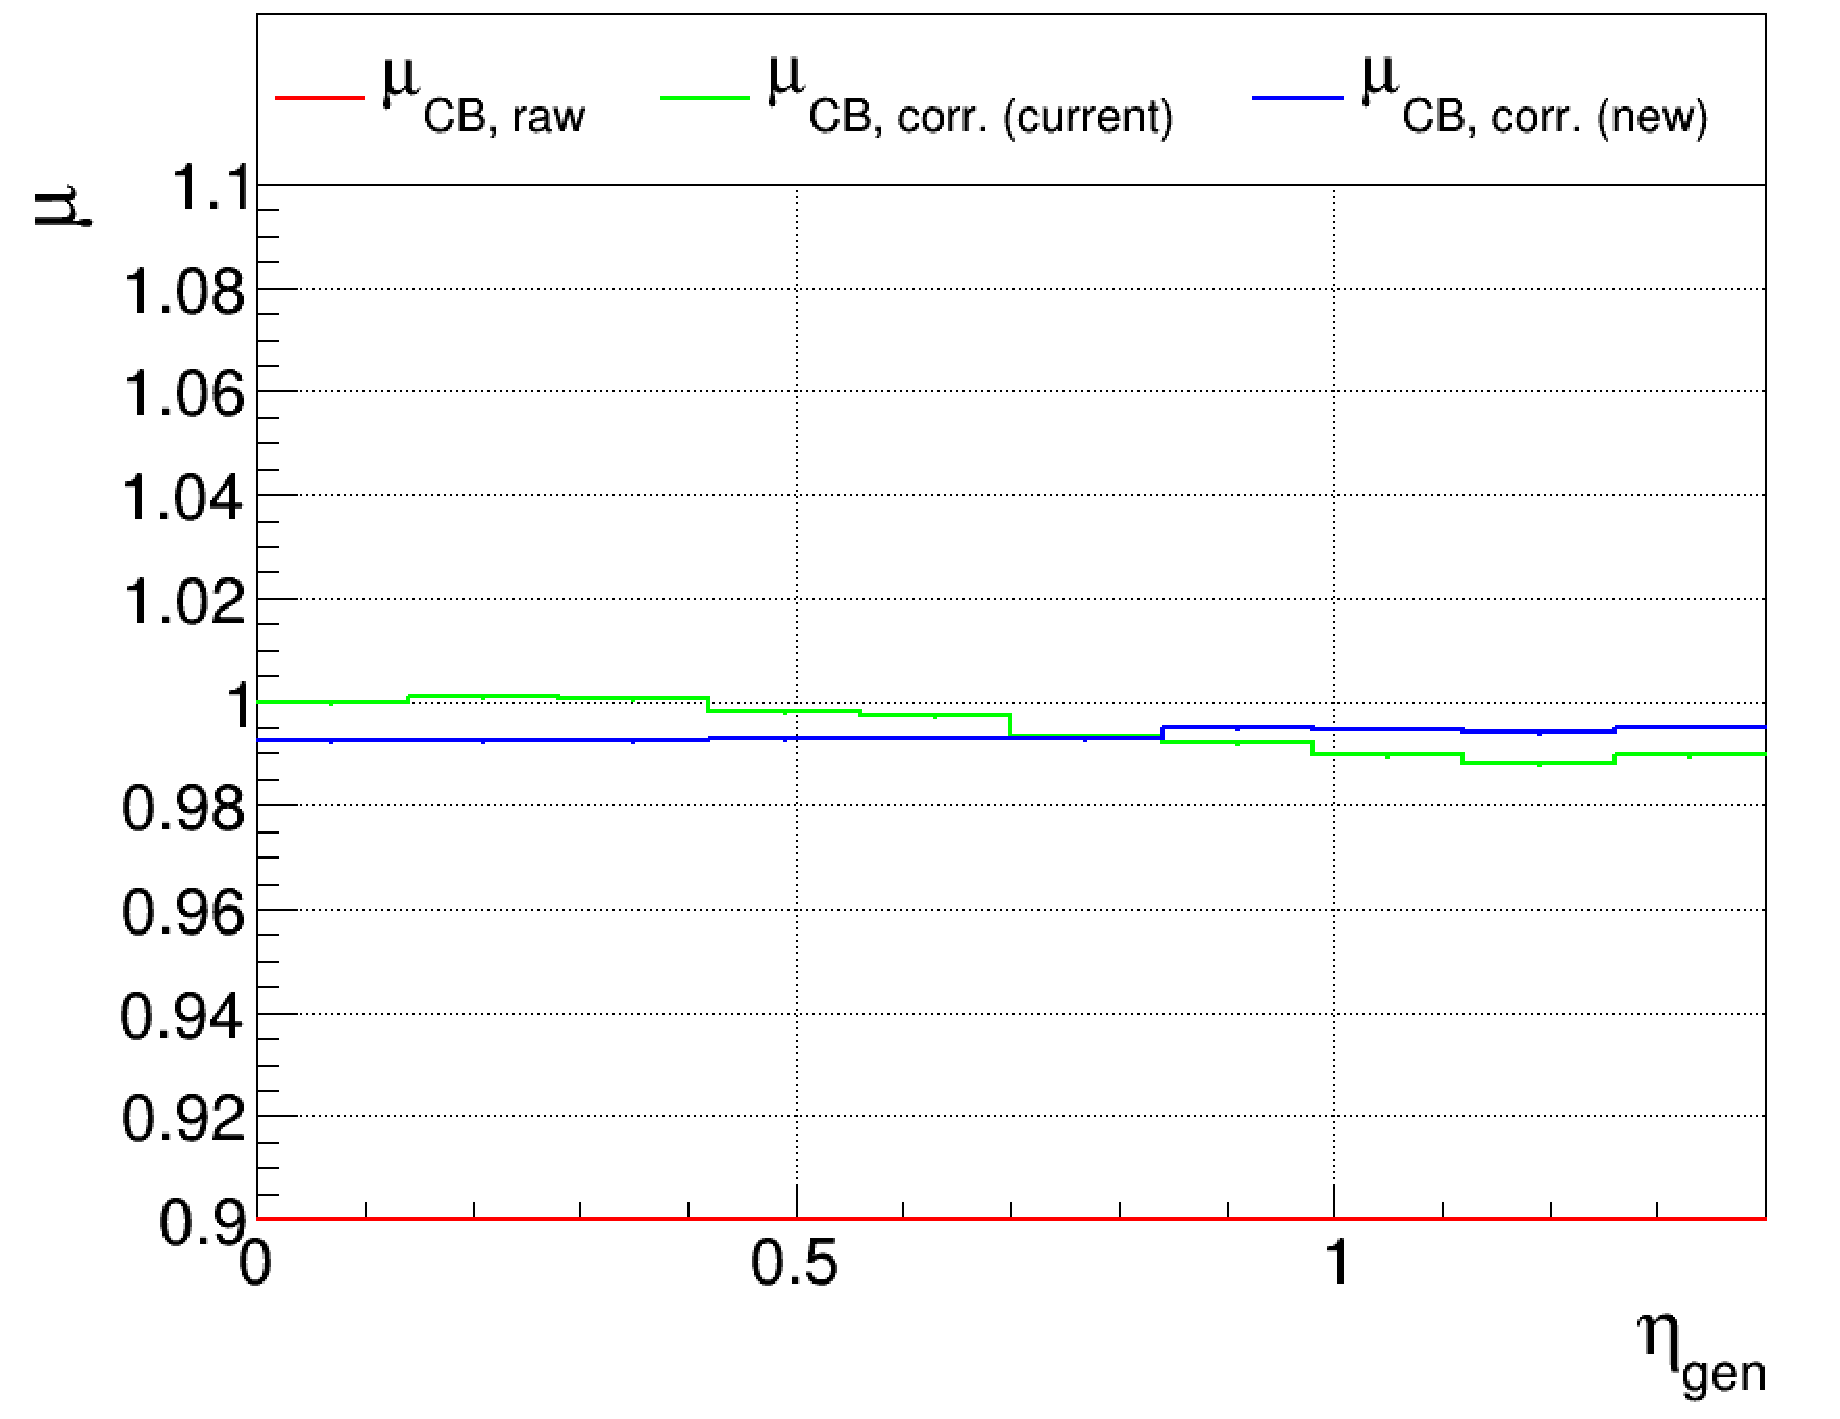
\includegraphics[width=0.495\textwidth]{./plots_pdf/ECAL_plots/plotsNOPU/EB/FULL/pdf/GENETA/EBFULL_GENETA_0005_0020_MuOverBins.pdf}
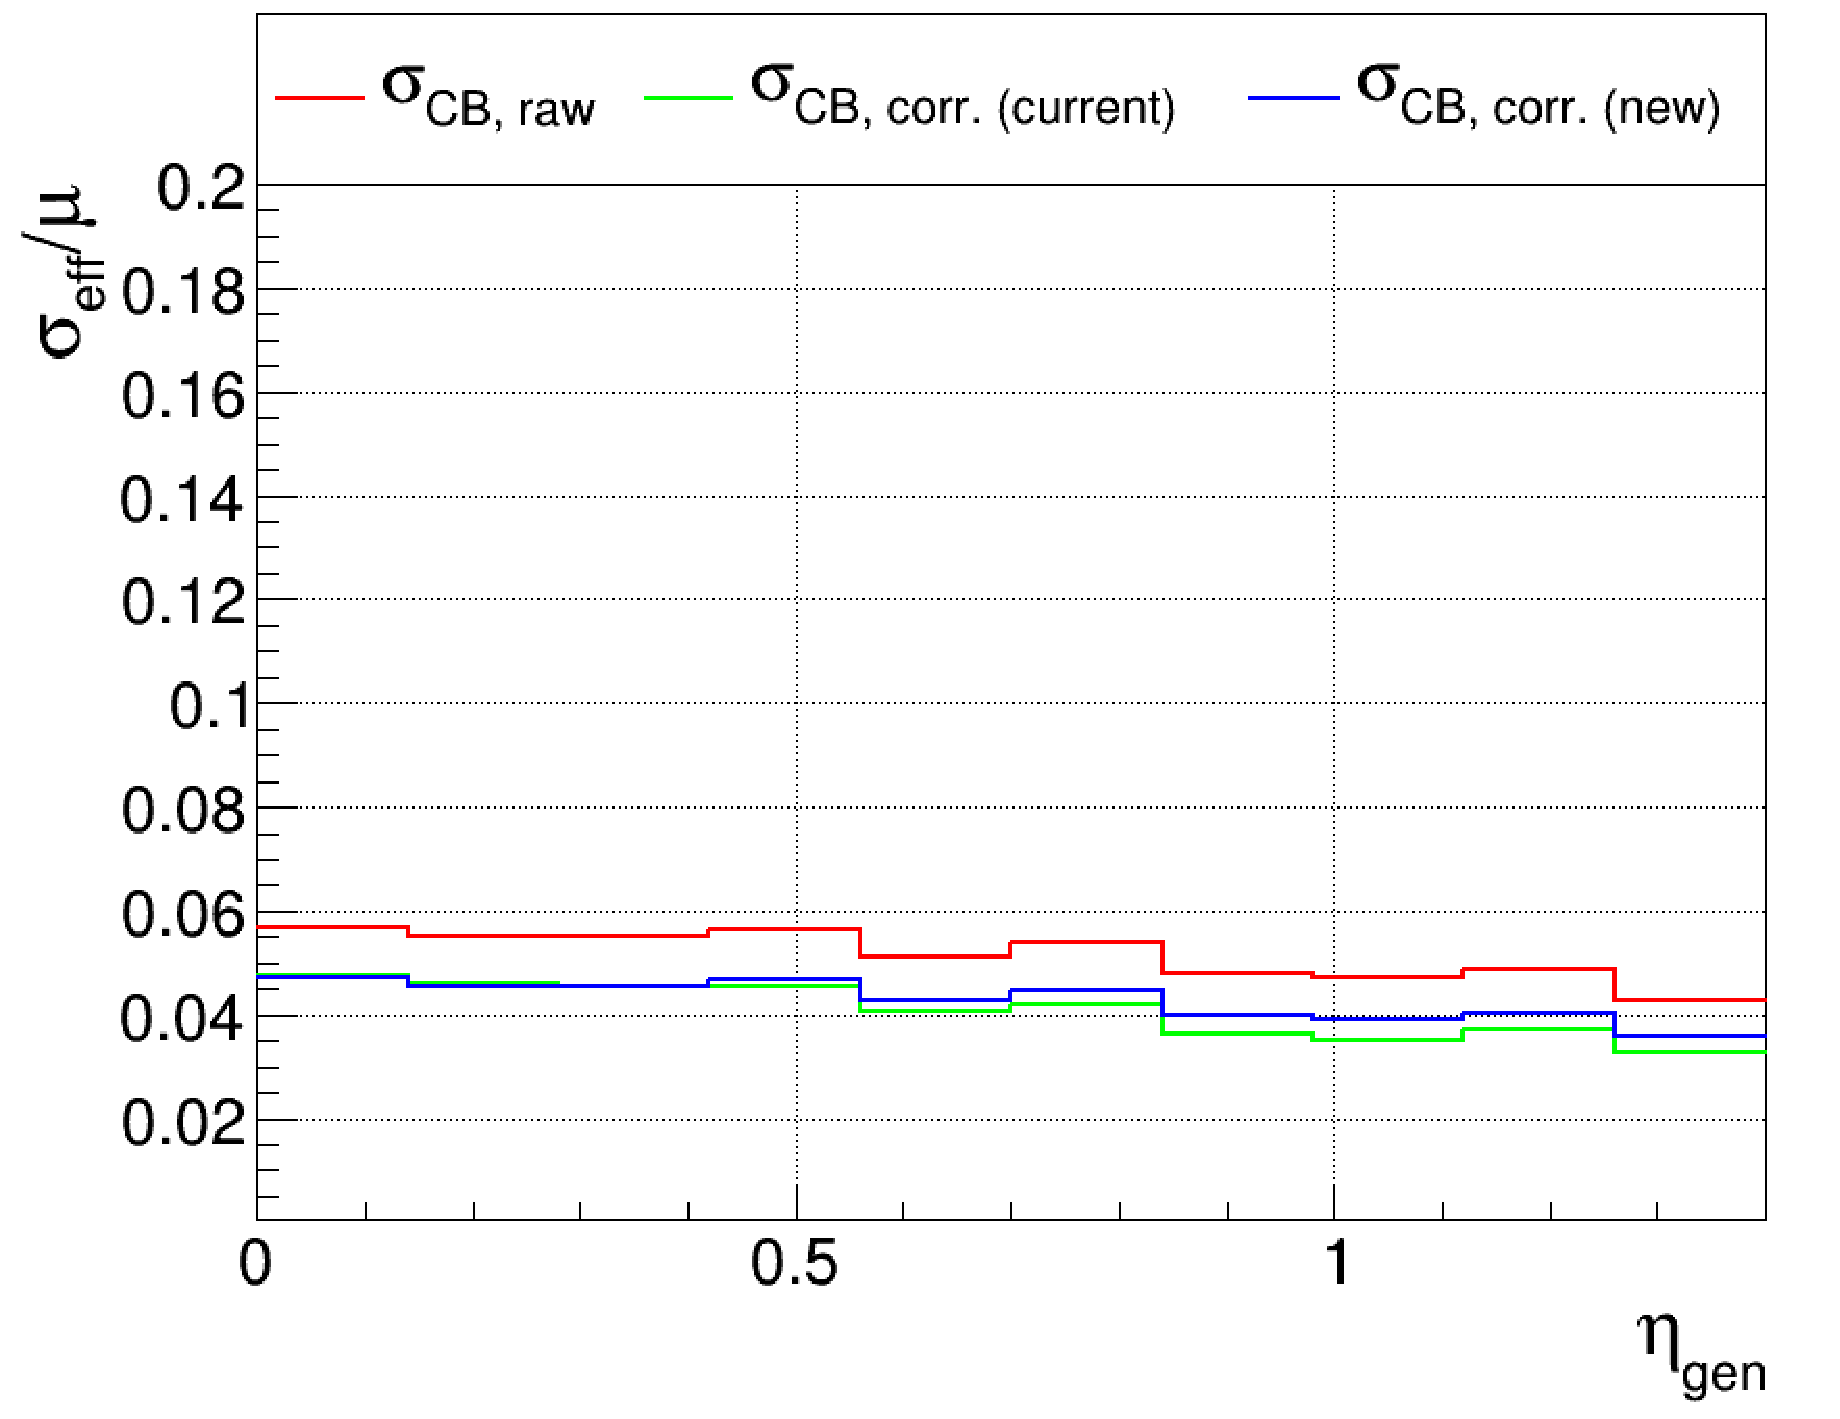
\includegraphics[width=0.495\textwidth]{./plots_pdf/ECAL_plots/plotsPU/EB/FULL/pdf/GENETA/EBFULL_GENETA_0005_0020_EffSigmaOverBins.pdf}
\caption{EB - Full Readout \pt 5-20}

%\begin{figure}
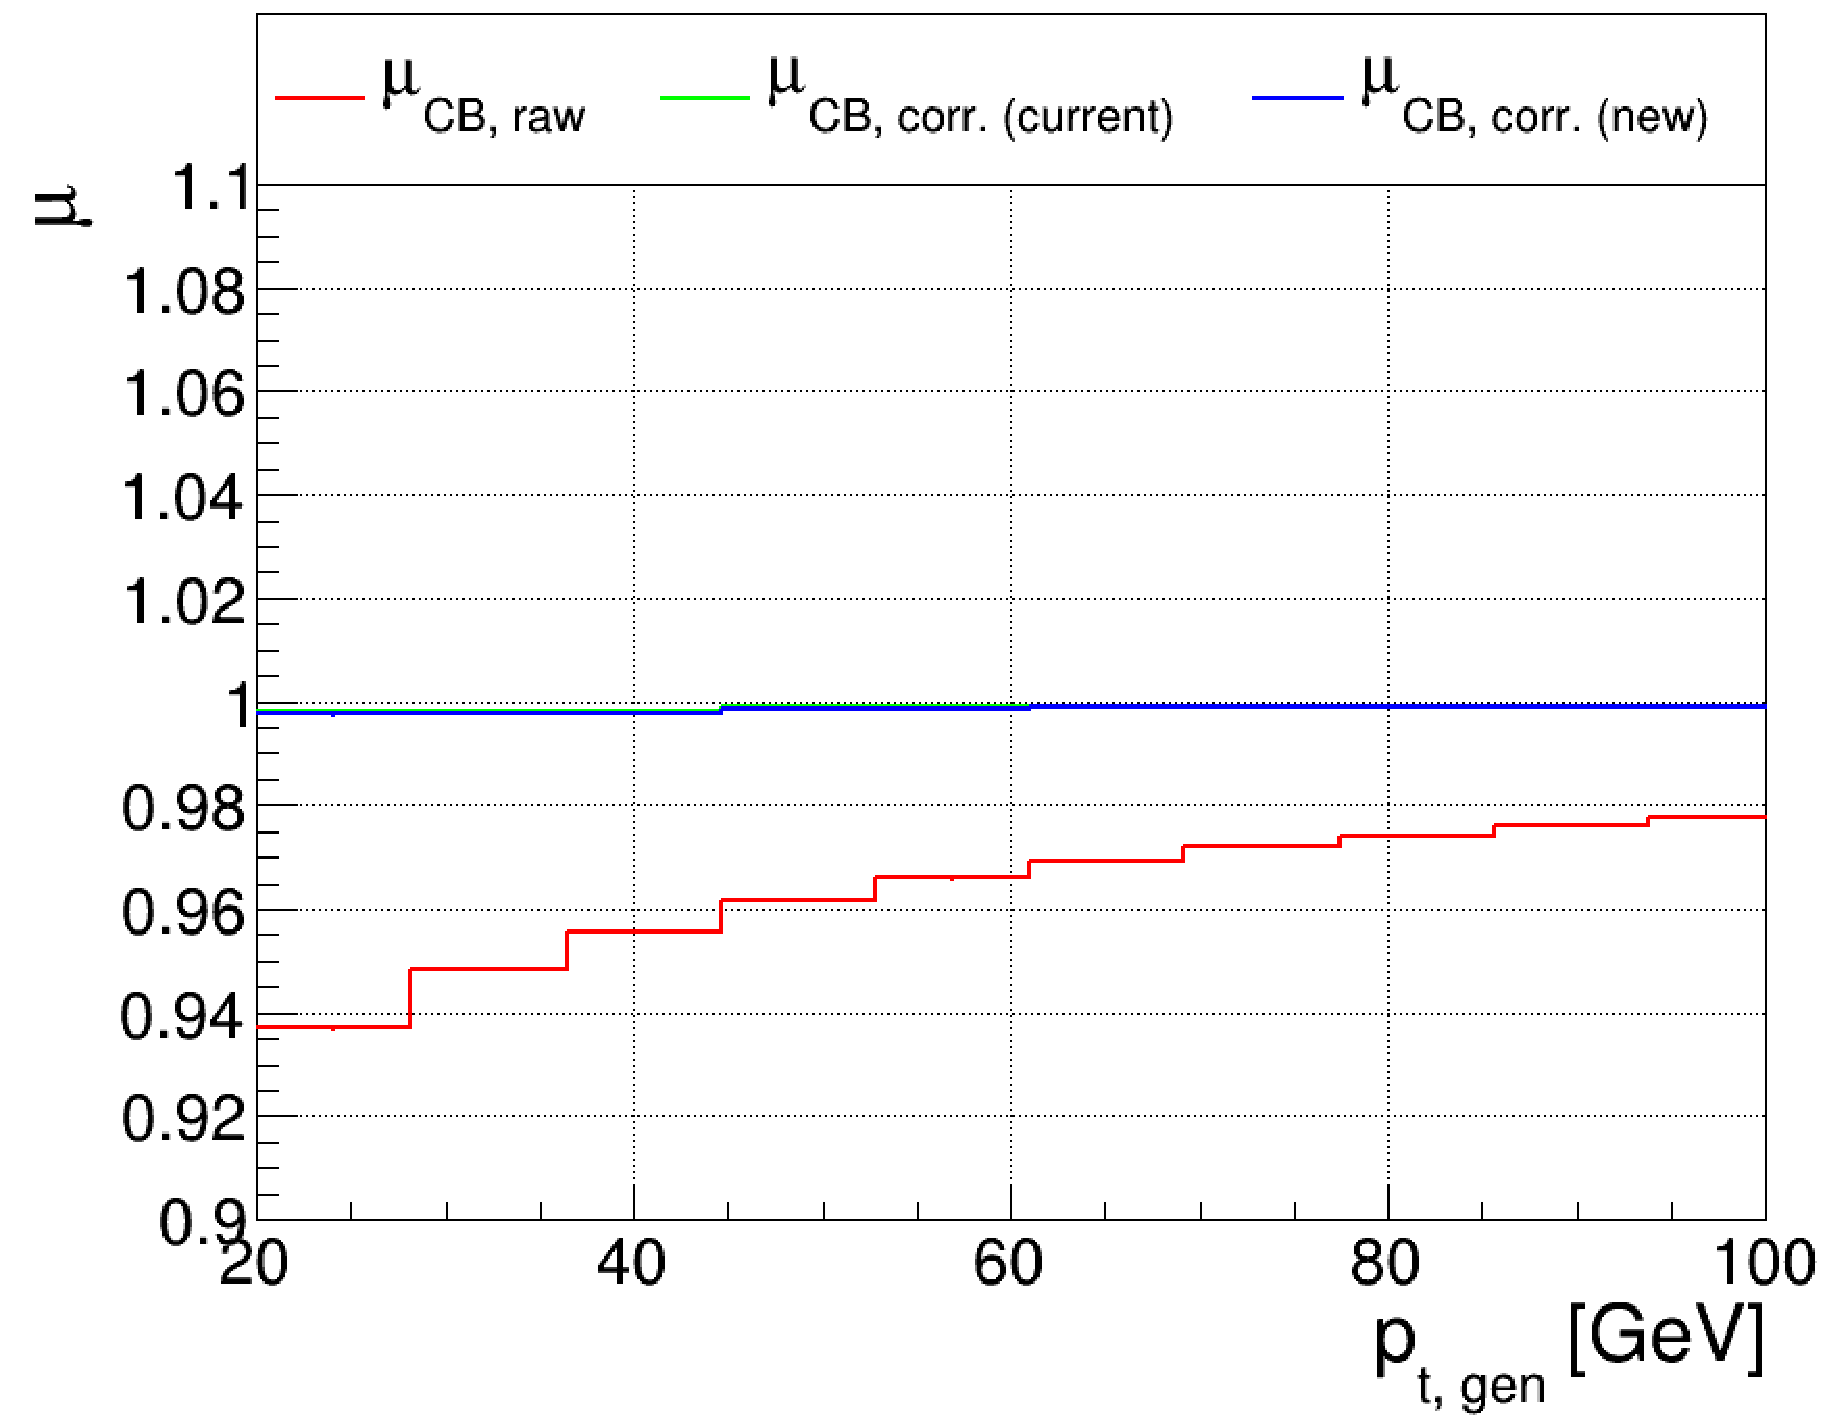
\includegraphics[width=0.495\textwidth]{./plots_pdf/ECAL_plots/plotsNOPU/EB/FULL/pdf/GENPT/EBFULL_GENPT_0020_0100_MuOverBins.pdf}
\includegraphics[width=0.495\textwidth]{./plots_pdf/ECAL_plots/plotsNOPU/EB/FULL/pdf/GENPT/EBFULL_GENPT_0020_0100_EffSigmaOverBins.pdf}

\includegraphics[width=0.495\textwidth]{./plots_pdf/ECAL_plots/plotsNOPU/EB/FULL/pdf/GENETA/EBFULL_GENETA_0020_0100_MuOverBins.pdf}
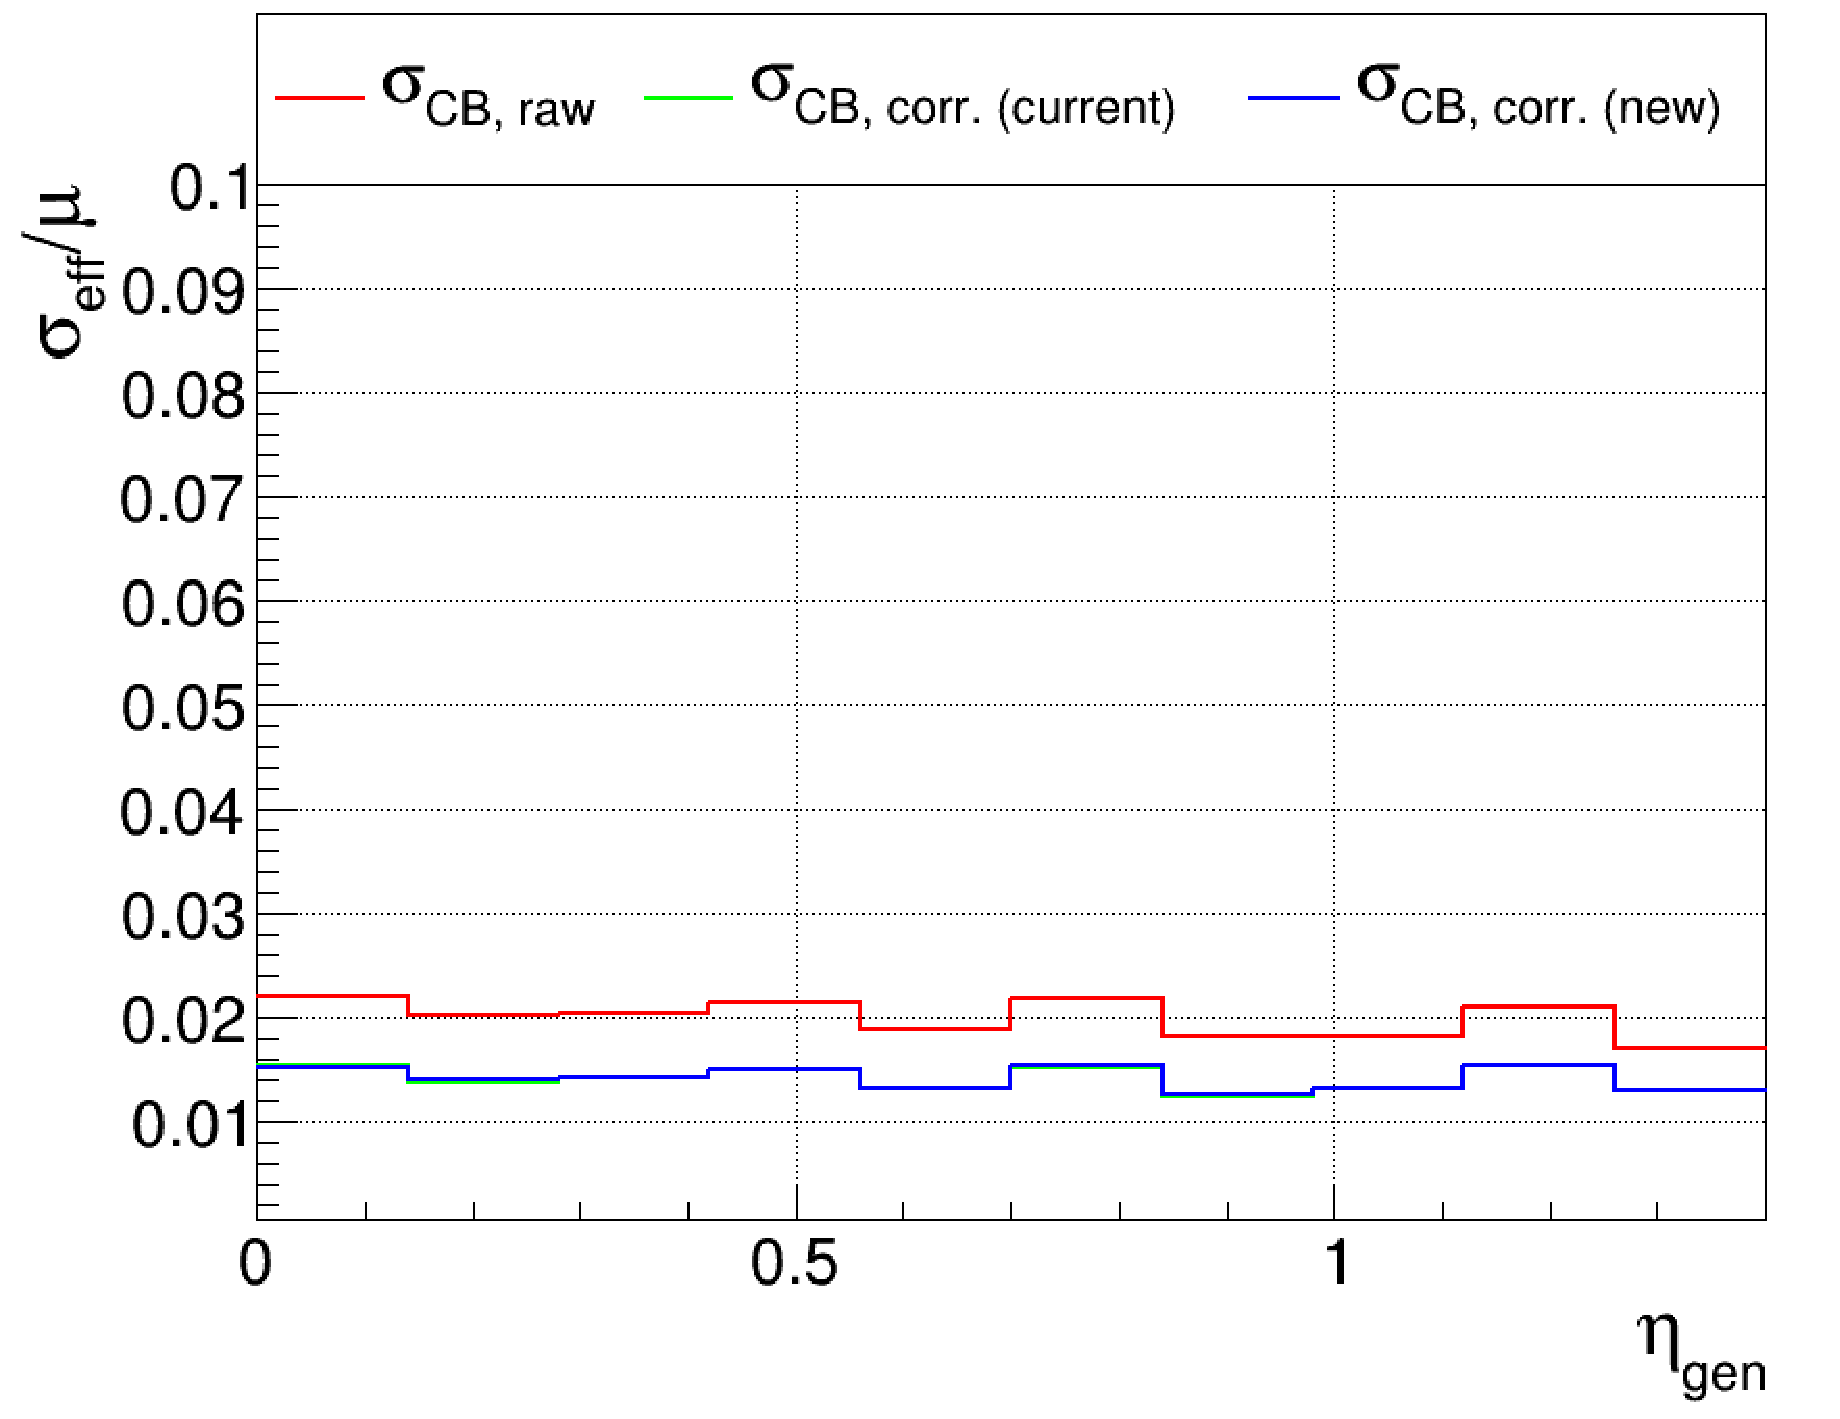
\includegraphics[width=0.495\textwidth]{./plots_pdf/ECAL_plots/plotsPU/EB/FULL/pdf/GENETA/EBFULL_GENETA_0020_0100_EffSigmaOverBins.pdf}
\caption{EB - Full Readout \pt 20-100}
\end{figure}


\begin{figure}
\includegraphics[width=0.495\textwidth]{./plots_pdf/ECAL_plots/plotsNOPU/EB/FULL/pdf/GENPT/EBFULL_GENPT_0100_0300_MuOverBins.pdf}
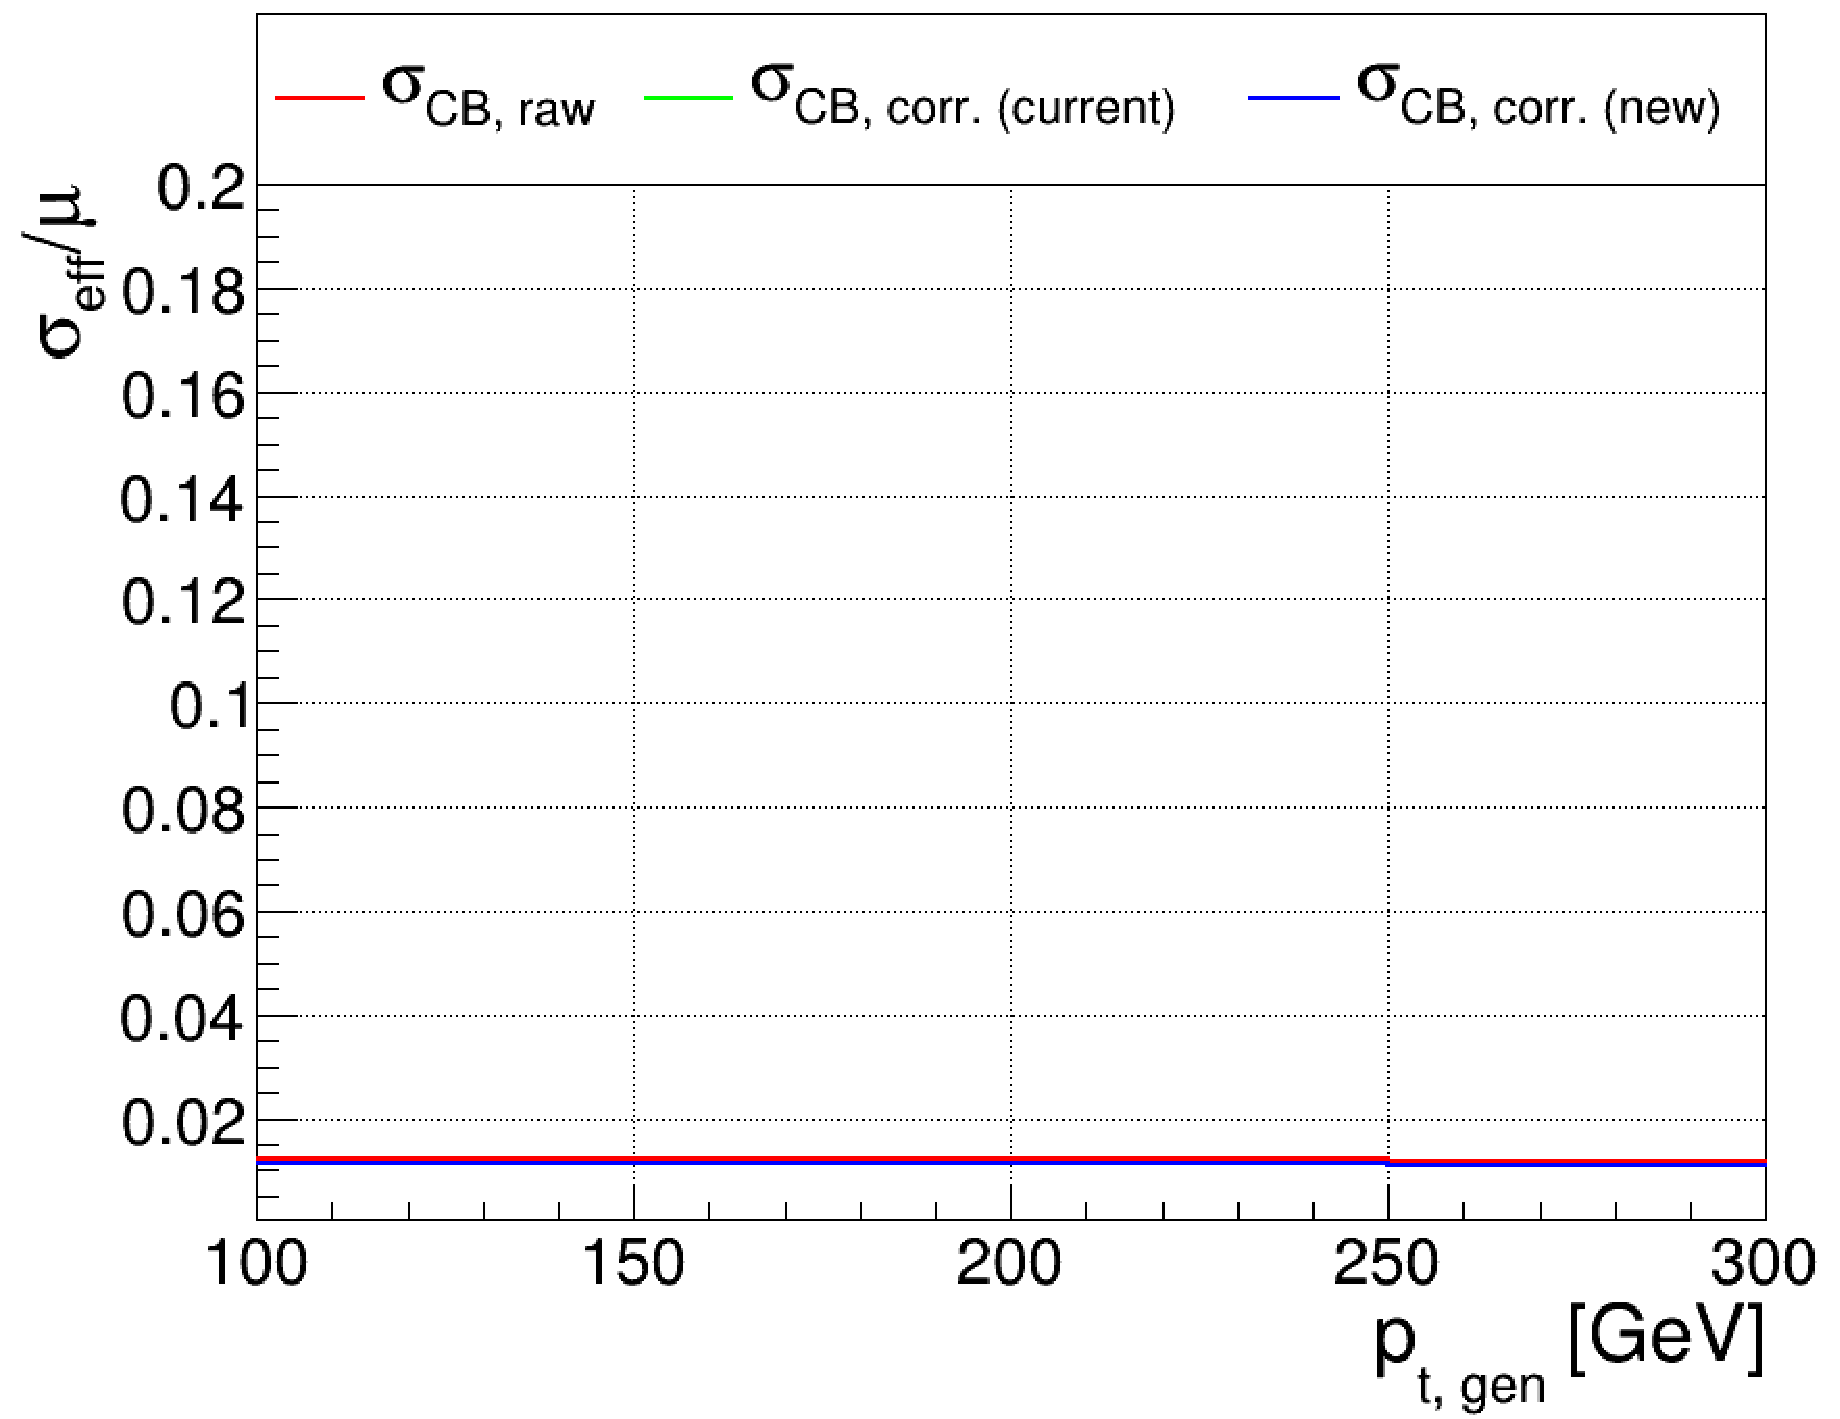
\includegraphics[width=0.495\textwidth]{./plots_pdf/ECAL_plots/plotsPU/EB/FULL/pdf/GENPT/EBFULL_GENPT_0100_0300_EffSigmaOverBins.pdf}


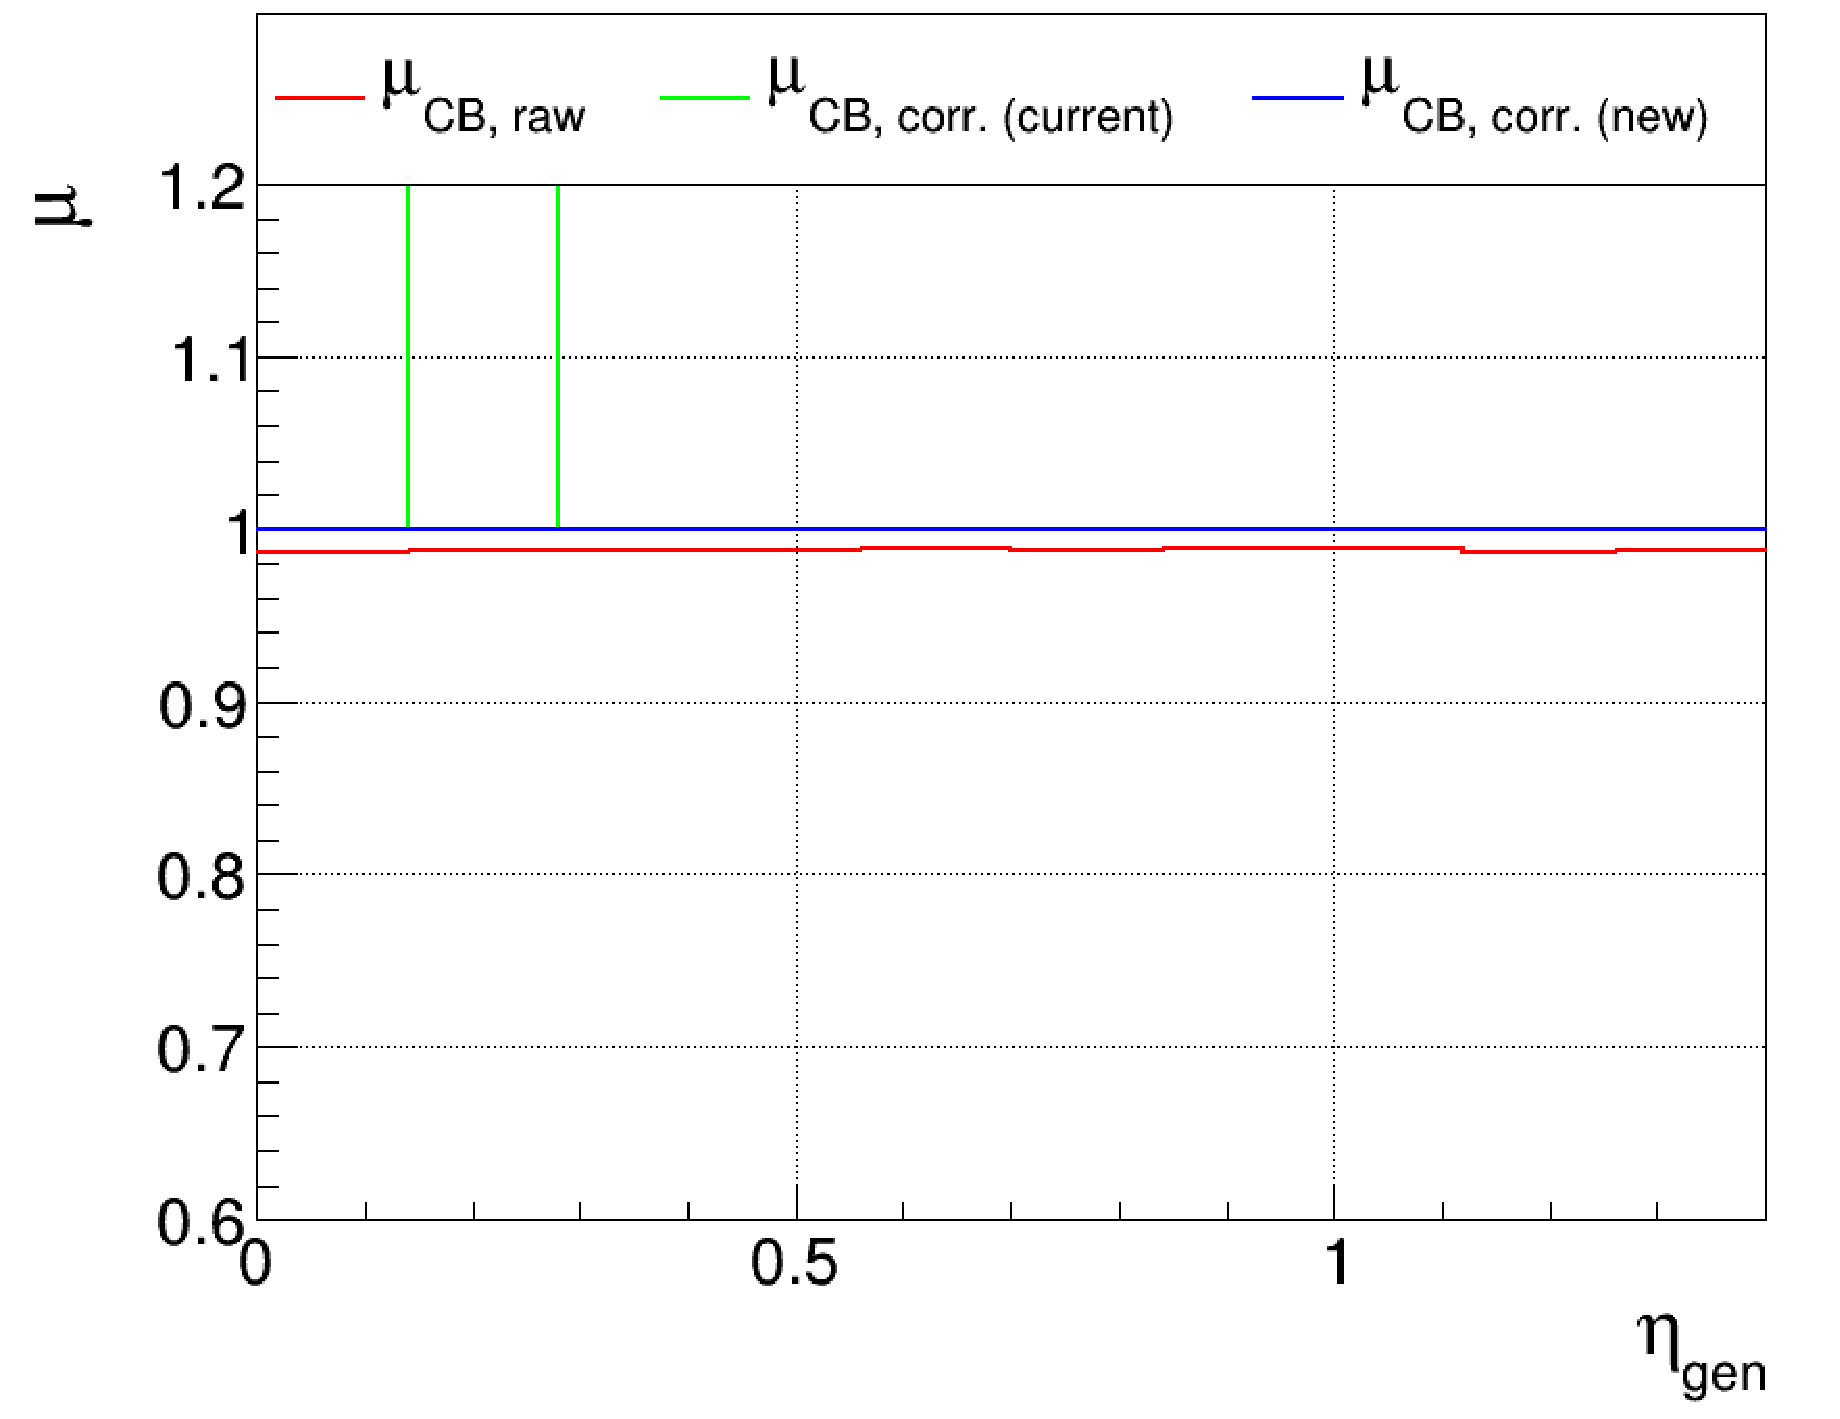
\includegraphics[width=0.495\textwidth]{./plots_pdf/ECAL_plots/plotsNOPU/EB/FULL/pdf/GENETA/EBFULL_GENETA_0100_0300_MuOverBins.pdf}
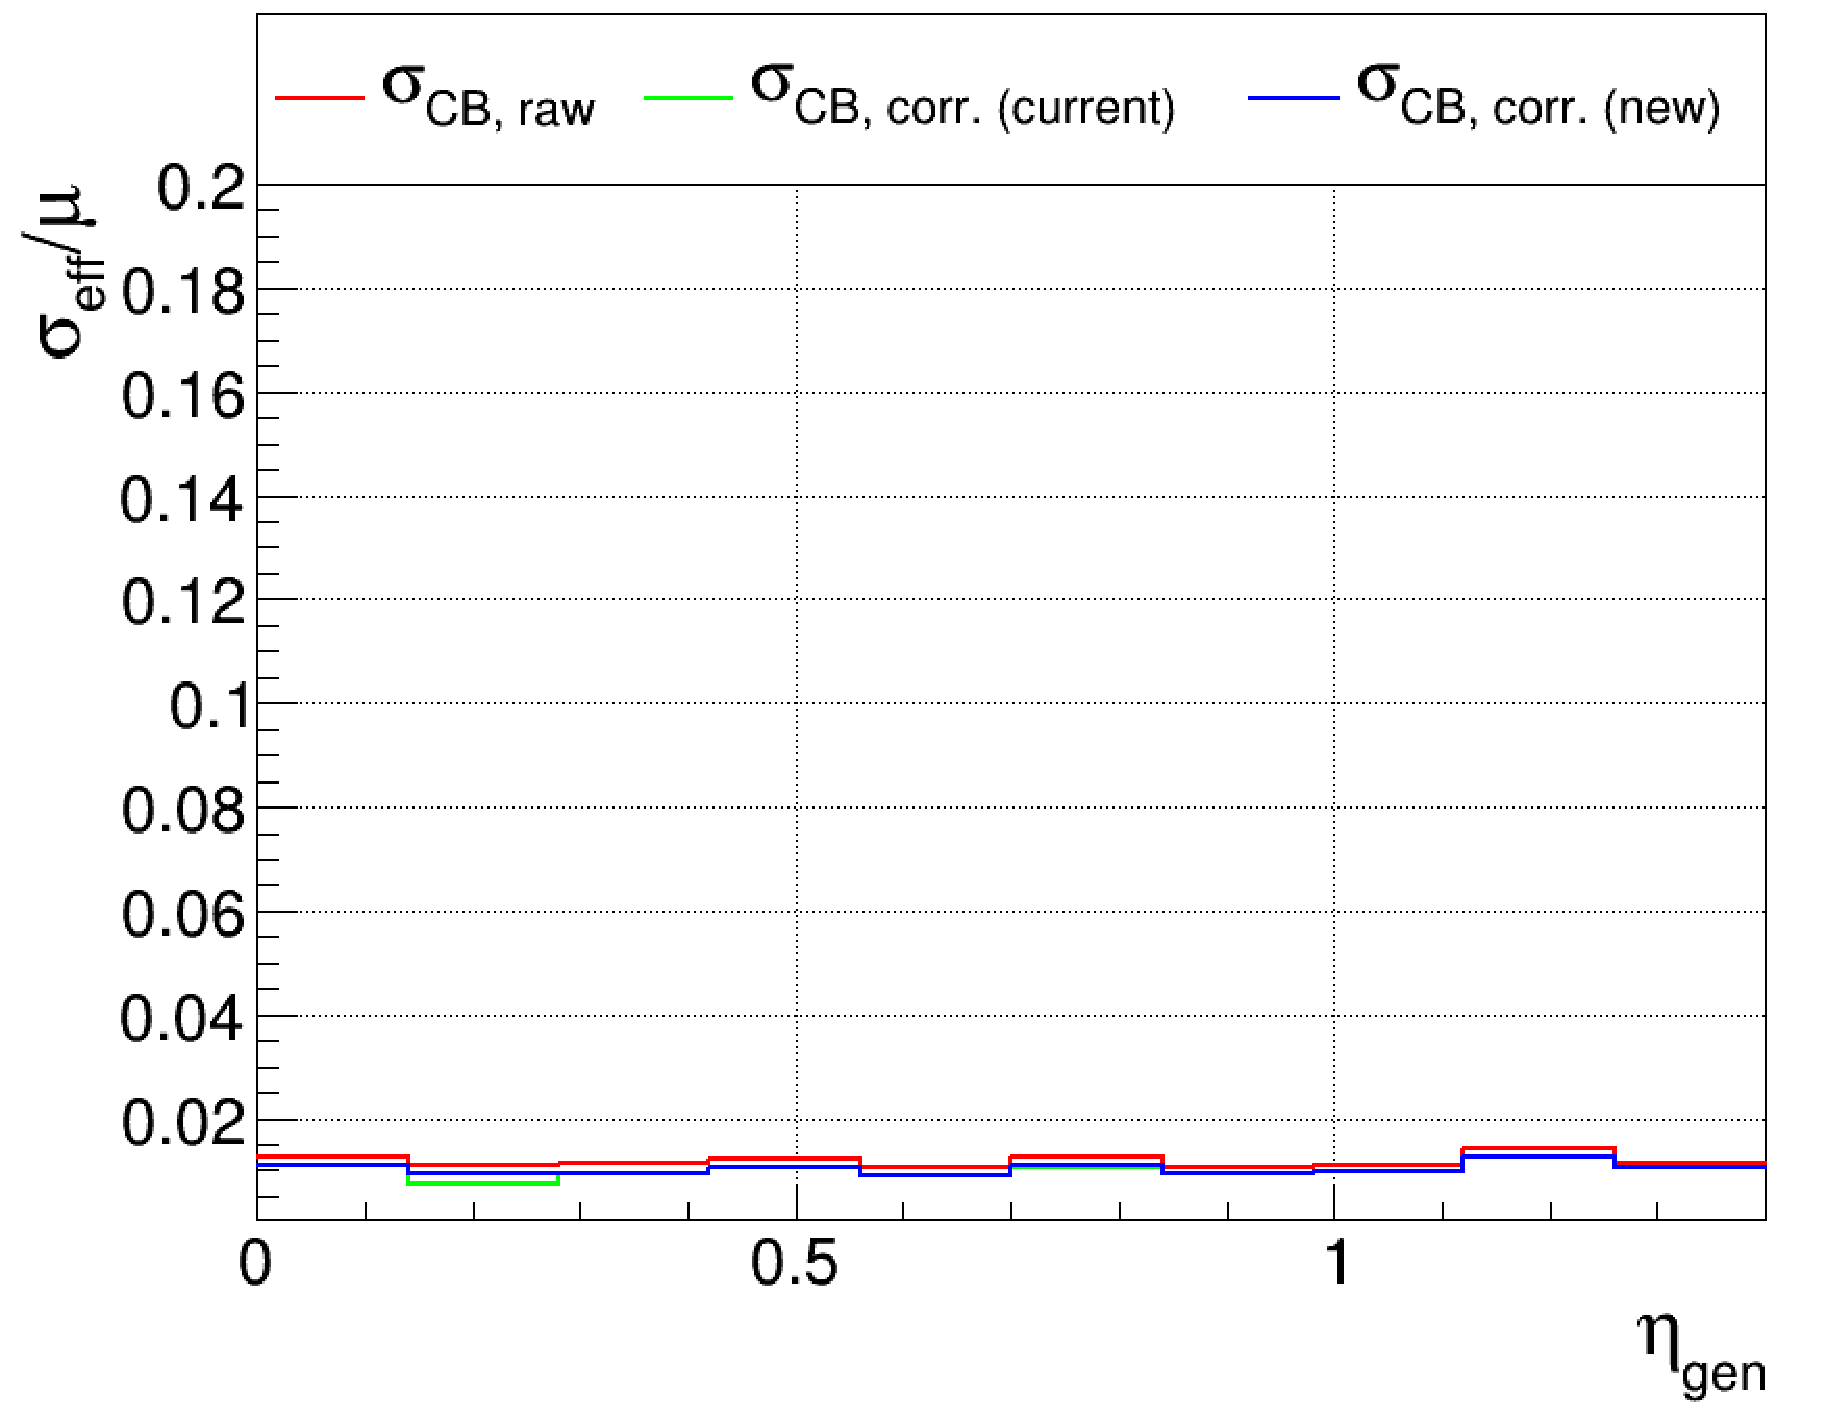
\includegraphics[width=0.495\textwidth]{./plots_pdf/ECAL_plots/plotsNOPU/EB/FULL/pdf/GENETA/EBFULL_GENETA_0100_0300_EffSigmaOverBins.pdf}
\caption{EB - Full Readout \pt 100-300}
\end{figure}




\begin{figure}
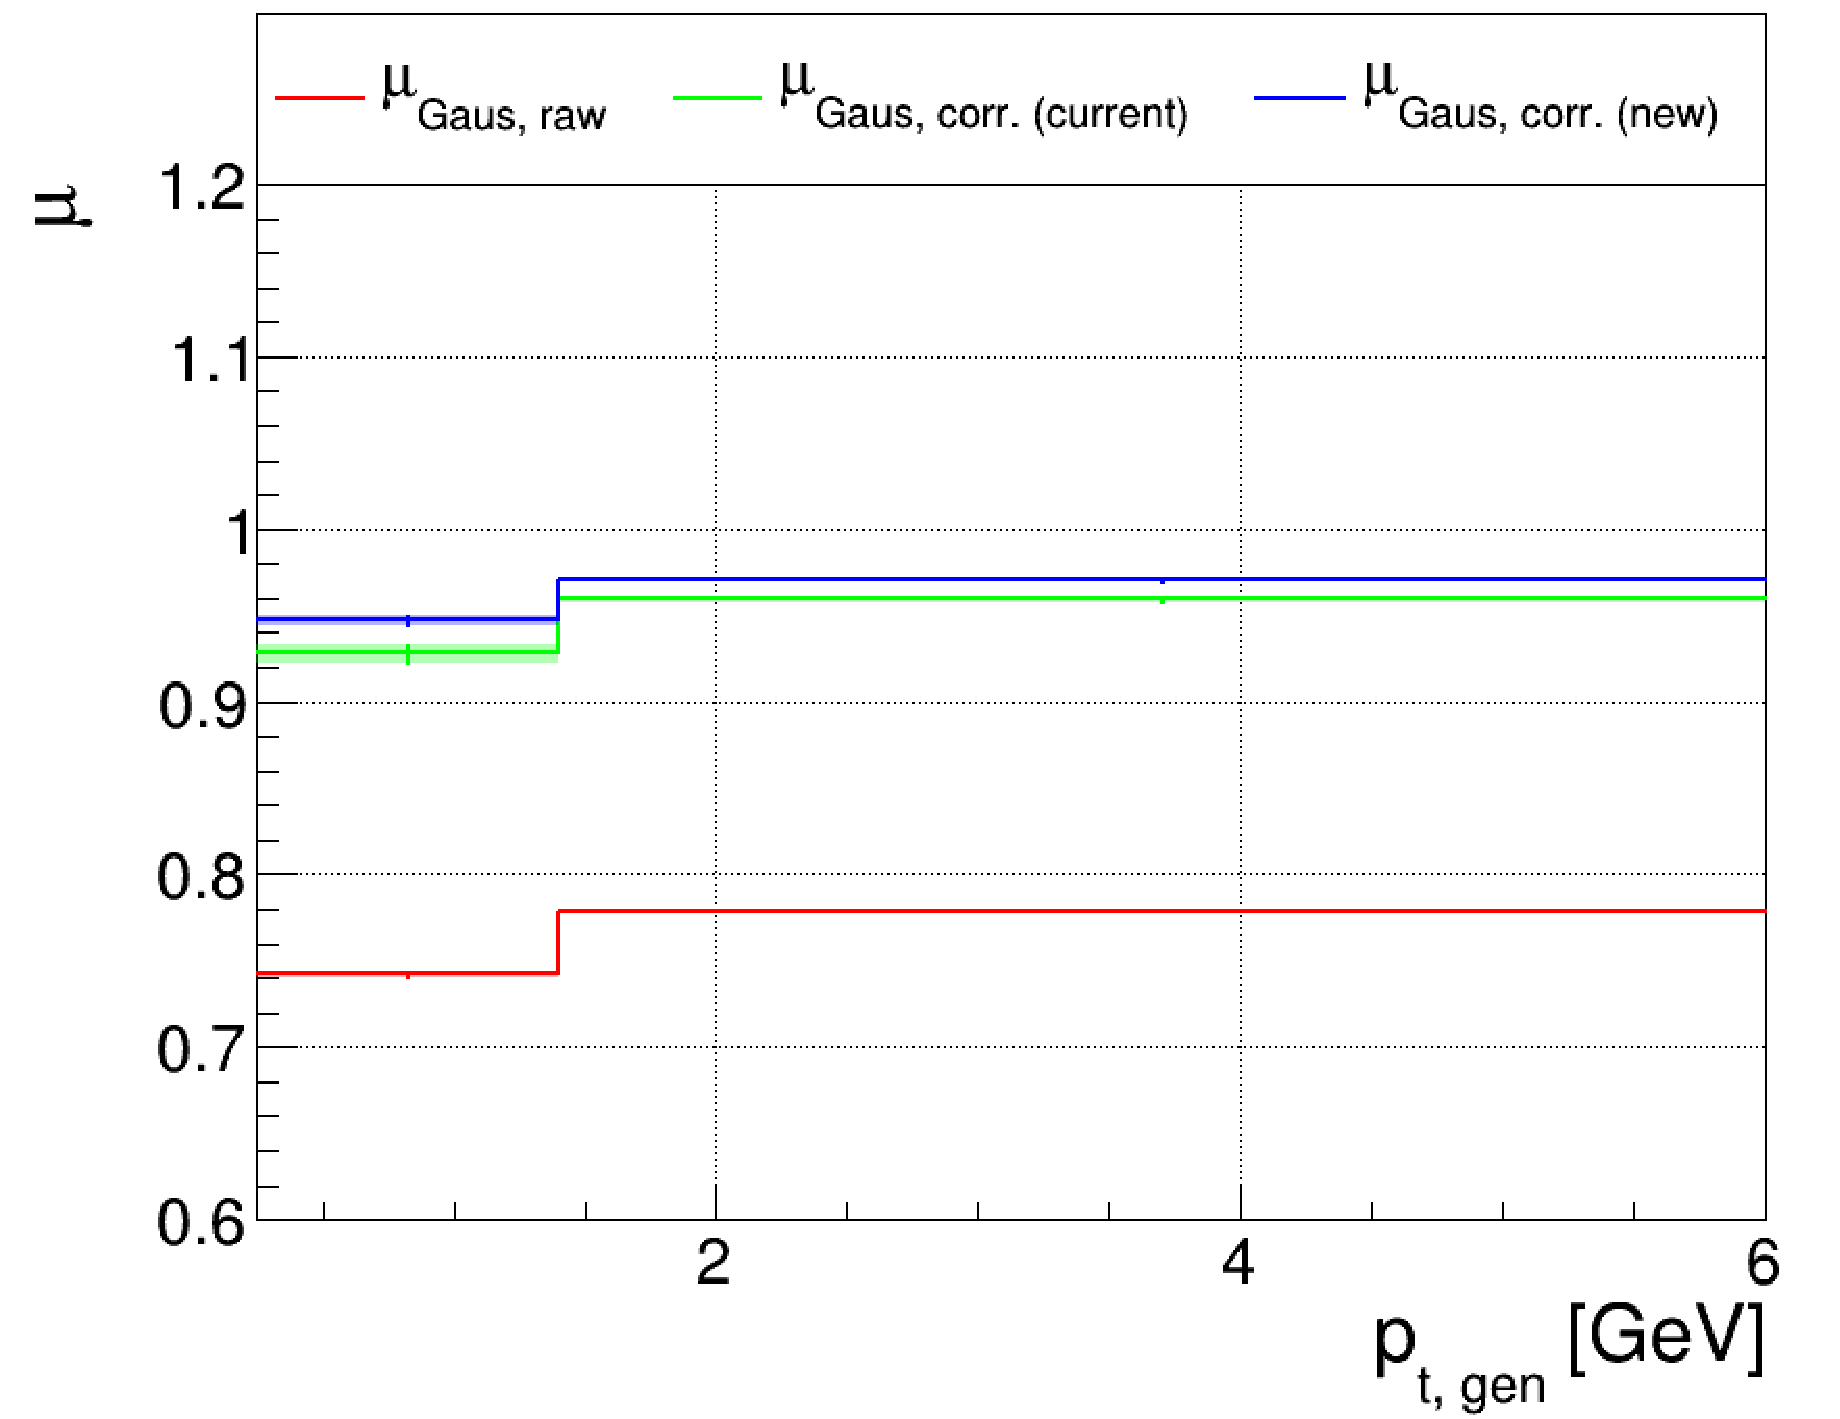
\includegraphics[width=0.495\textwidth]{./plots_pdf/ECAL_plots/plotsNOPU/EB/ZS/pdf/GENPT/EBZS_GENPT_0000_0006_MuOverBins.pdf}
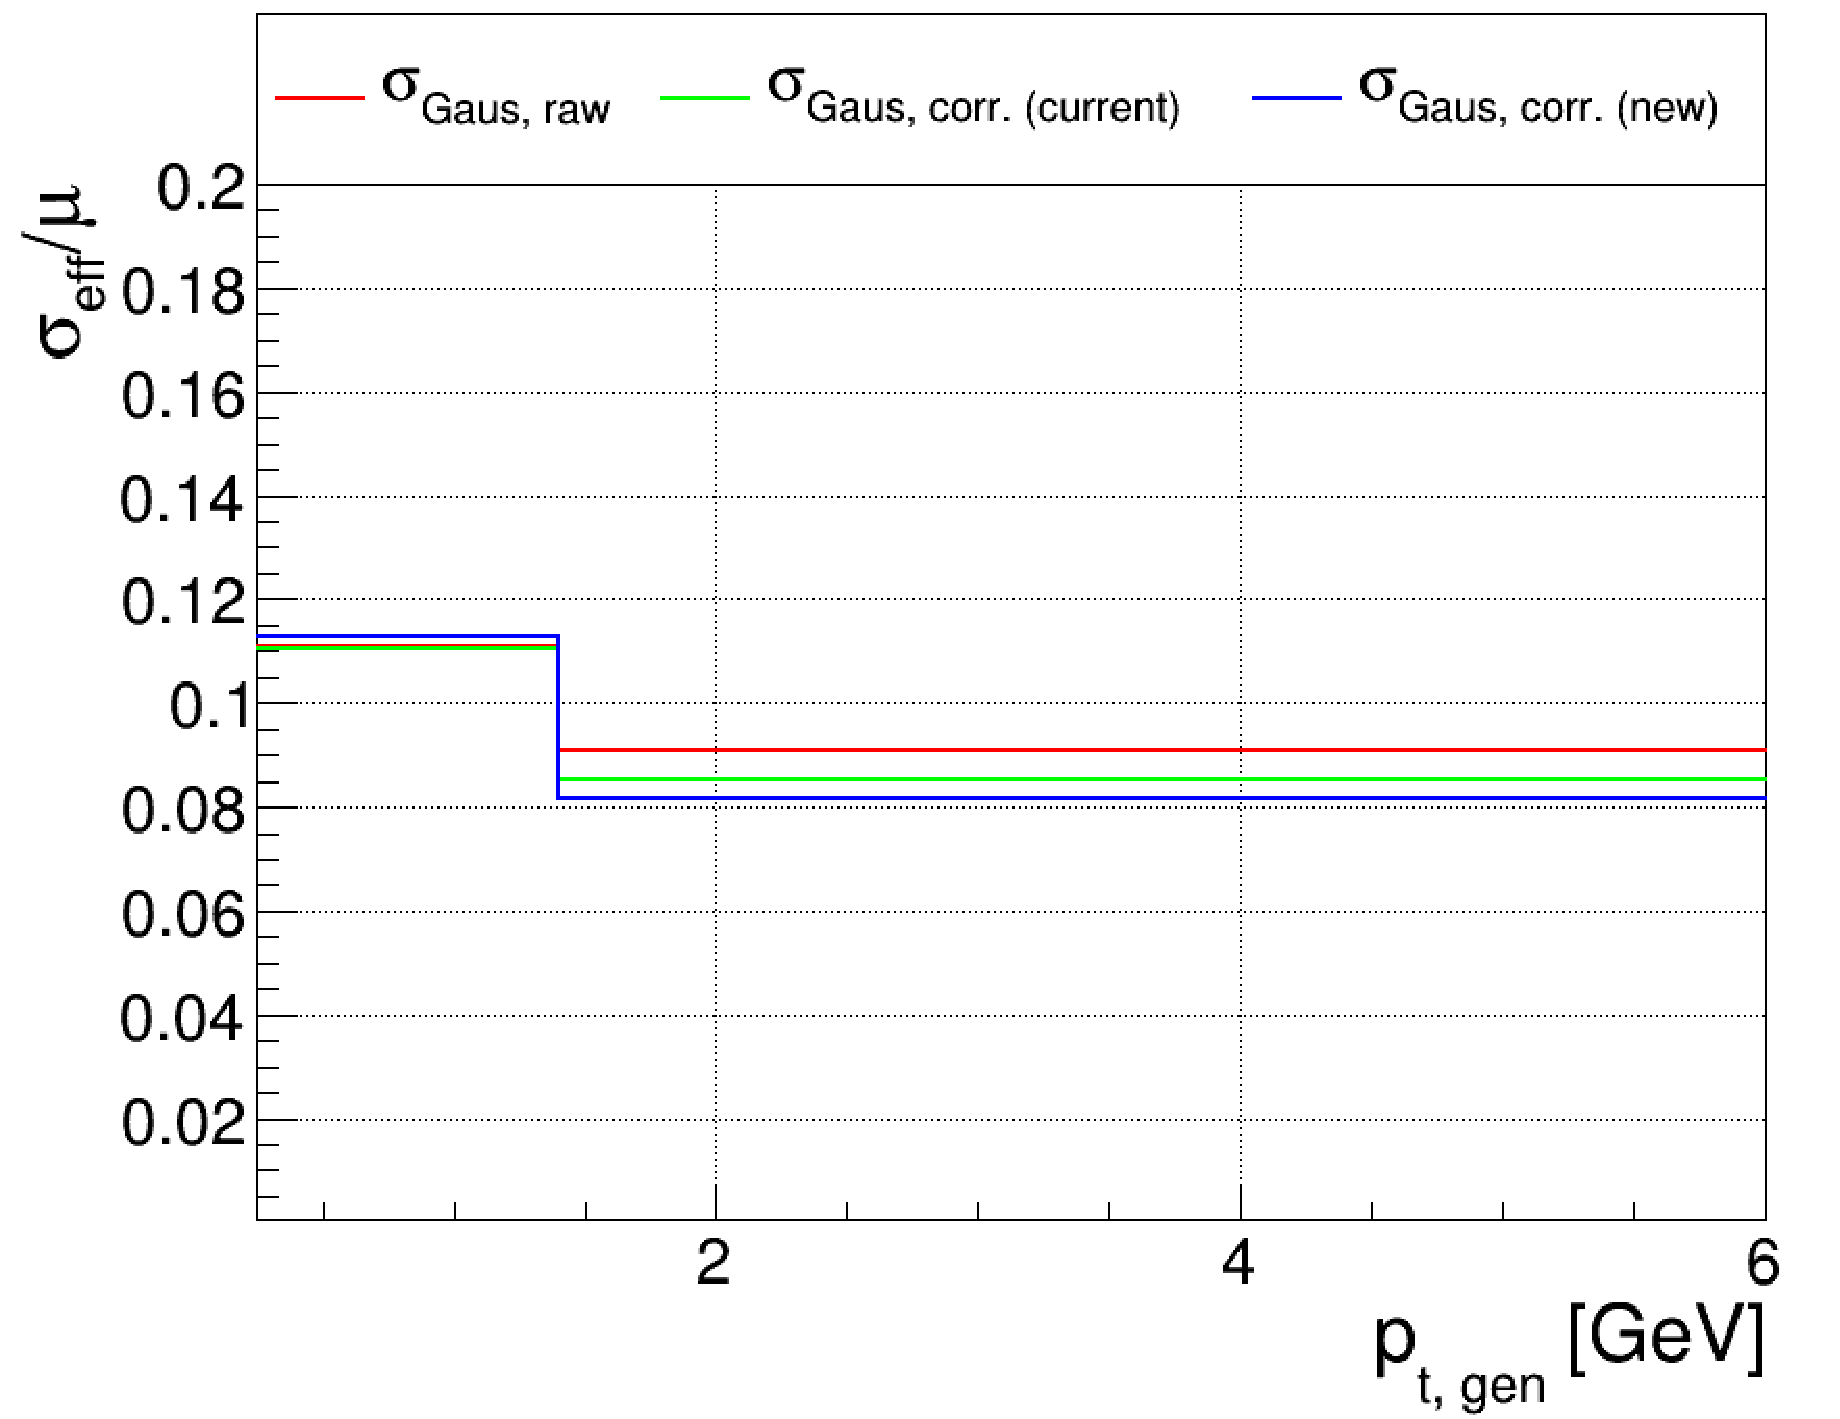
\includegraphics[width=0.495\textwidth]{./plots_pdf/ECAL_plots/plotsNOPU/EB/ZS/pdf/GENPT/EBZS_GENPT_0000_0006_EffSigmaOverBins.pdf}

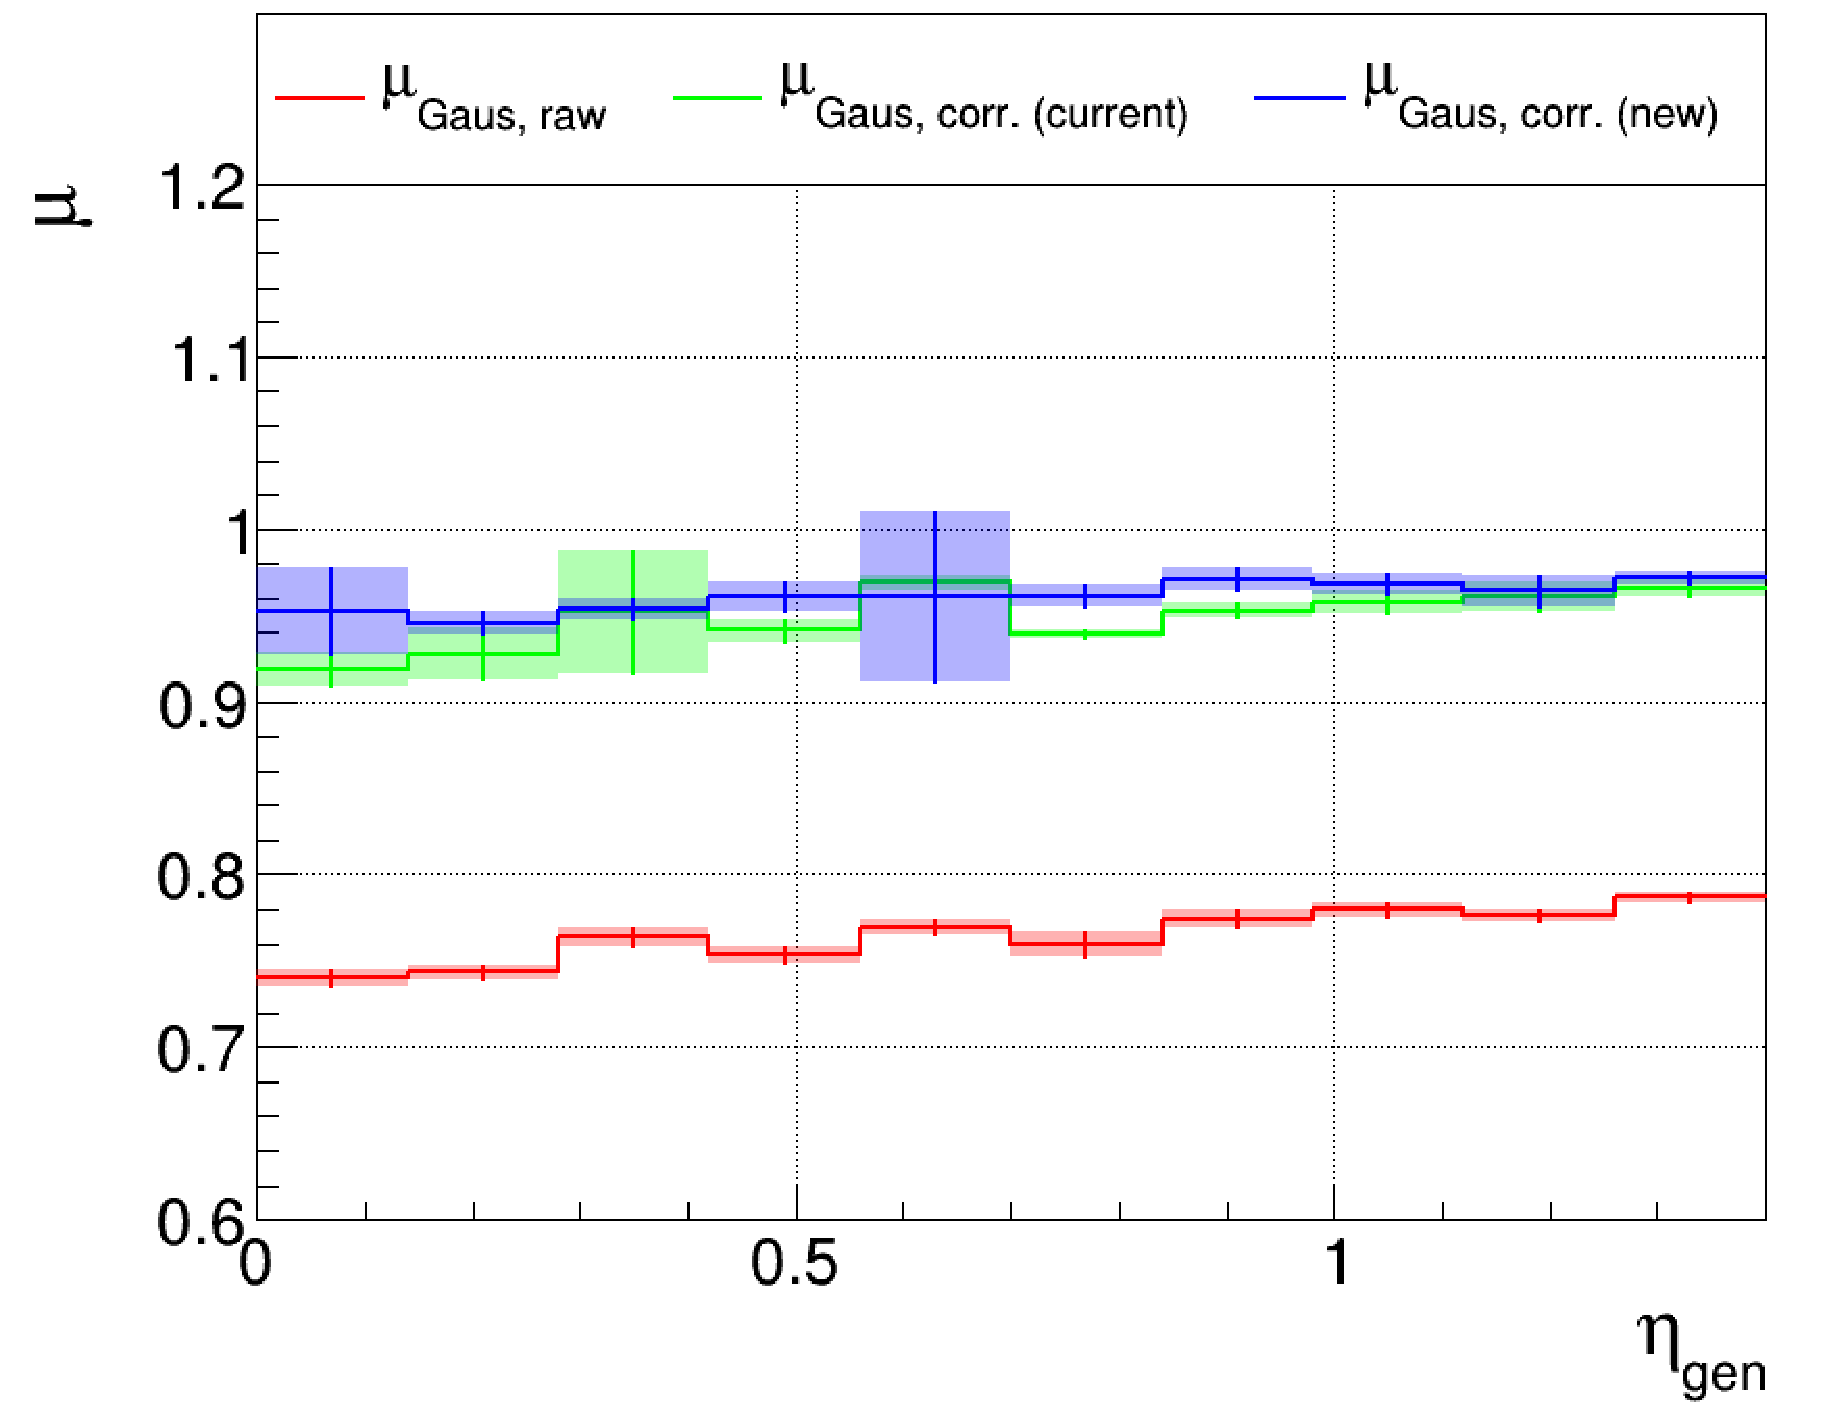
\includegraphics[width=0.495\textwidth]{./plots_pdf/ECAL_plots/plotsNOPU/EB/ZS/pdf/GENETA/EBZS_GENETA_0000_0006_MuOverBins.pdf}
\includegraphics[width=0.495\textwidth]{./plots_pdf/ECAL_plots/plotsNOPU/EB/ZS/pdf/GENETA/EBZS_GENETA_0000_0006_EffSigmaOverBins.pdf}
\caption[]{EB - ZS Readout \pt 0--6\GeV.}
\end{figure}

%% \begin{figure}
%% \includegraphics[width=0.495\textwidth]{./plots_pdf/ECAL_plots/plotsNOPU/EB/ZS/pdf/GENPT/EBZS_GENPT_0006_0025_MuOverBins.pdf}
%% 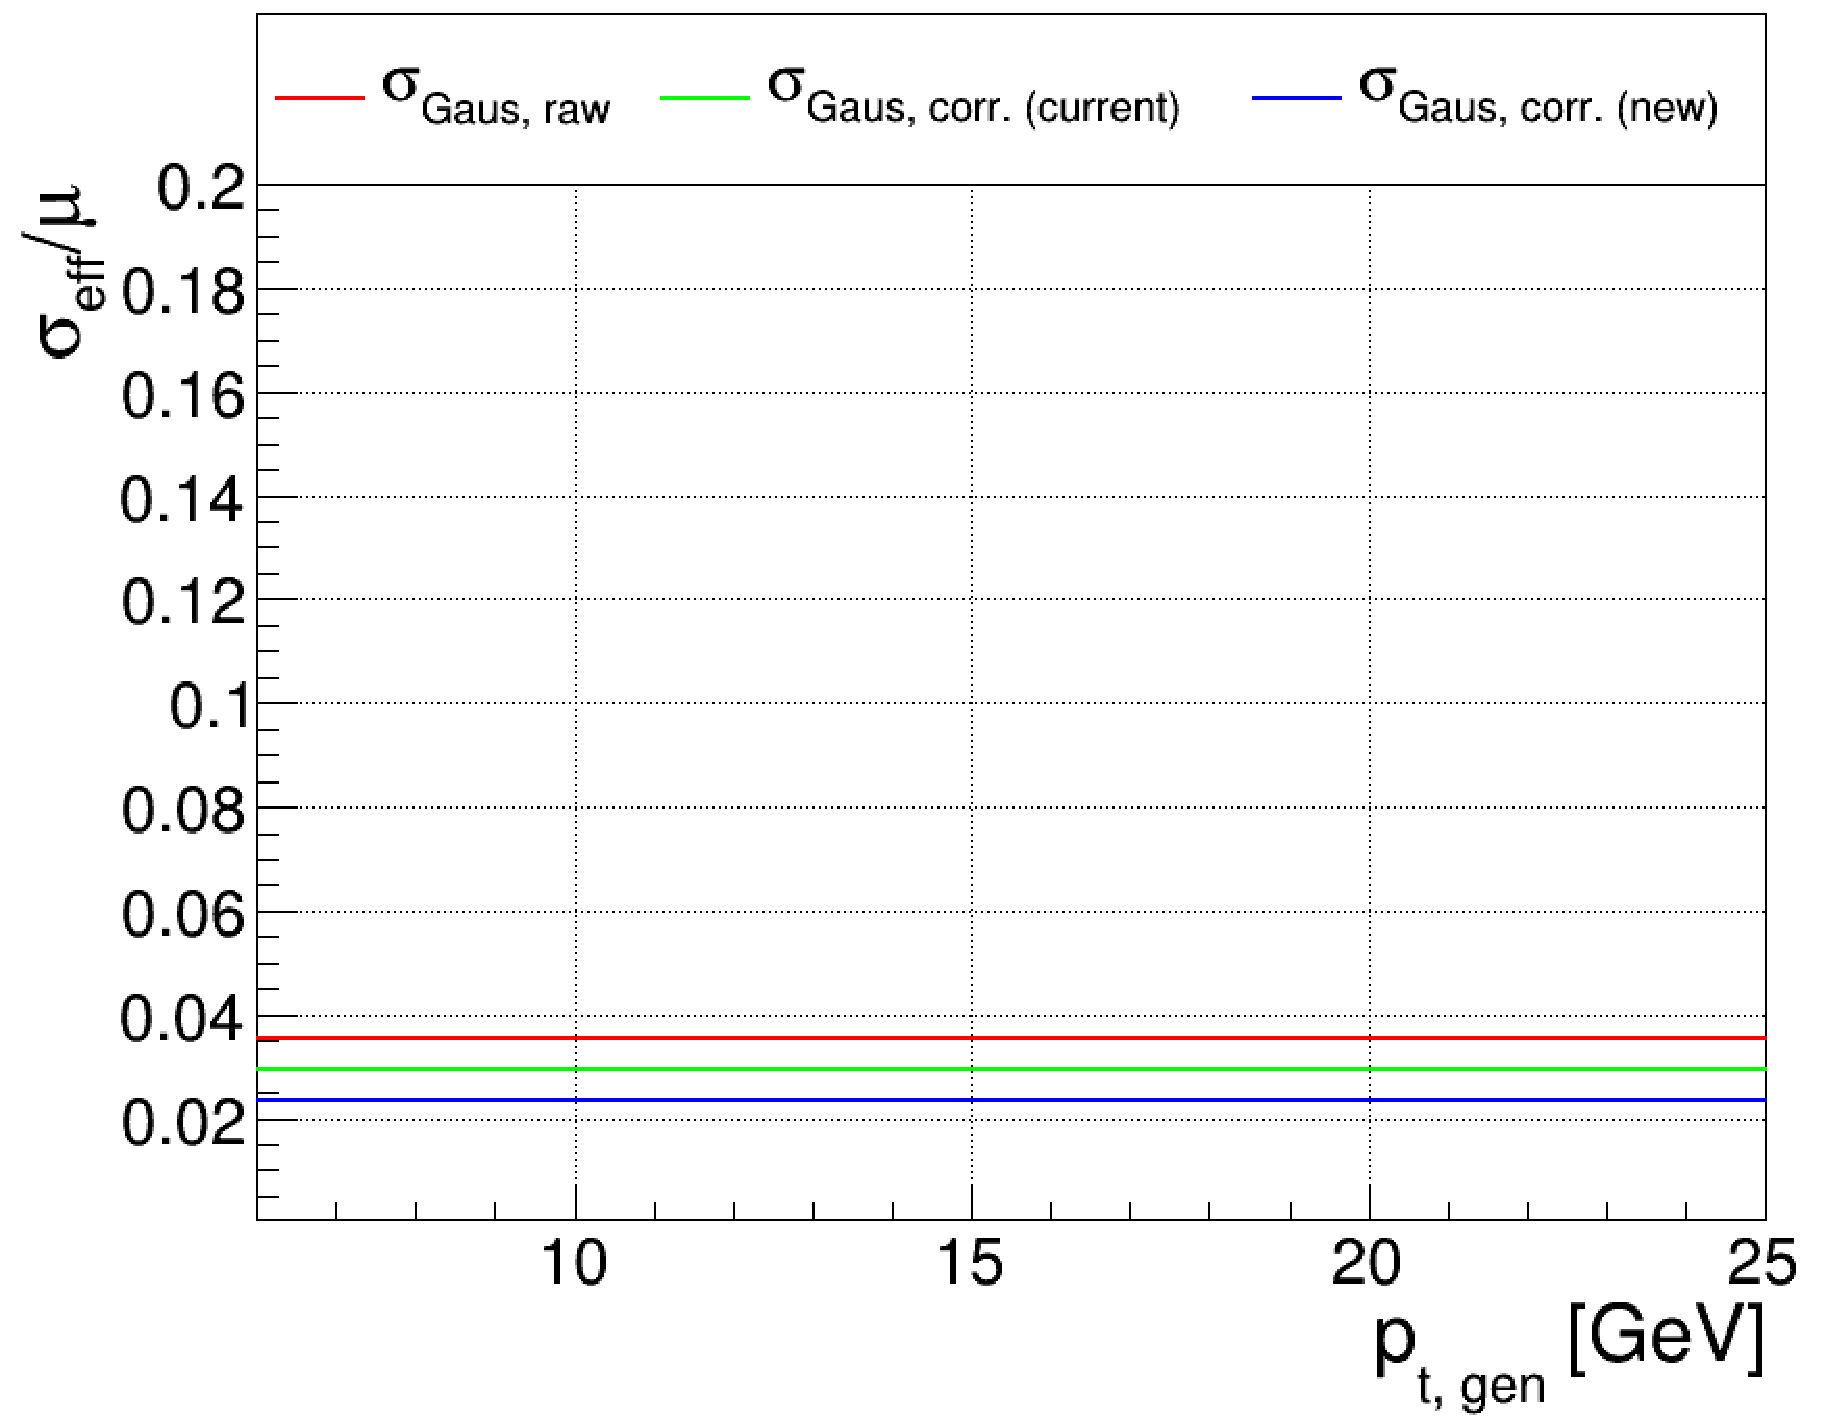
\includegraphics[width=0.495\textwidth]{./plots_pdf/ECAL_plots/plotsNOPU/EB/ZS/pdf/GENPT/EBZS_GENPT_0006_0025_EffSigmaOverBins.pdf}

%% 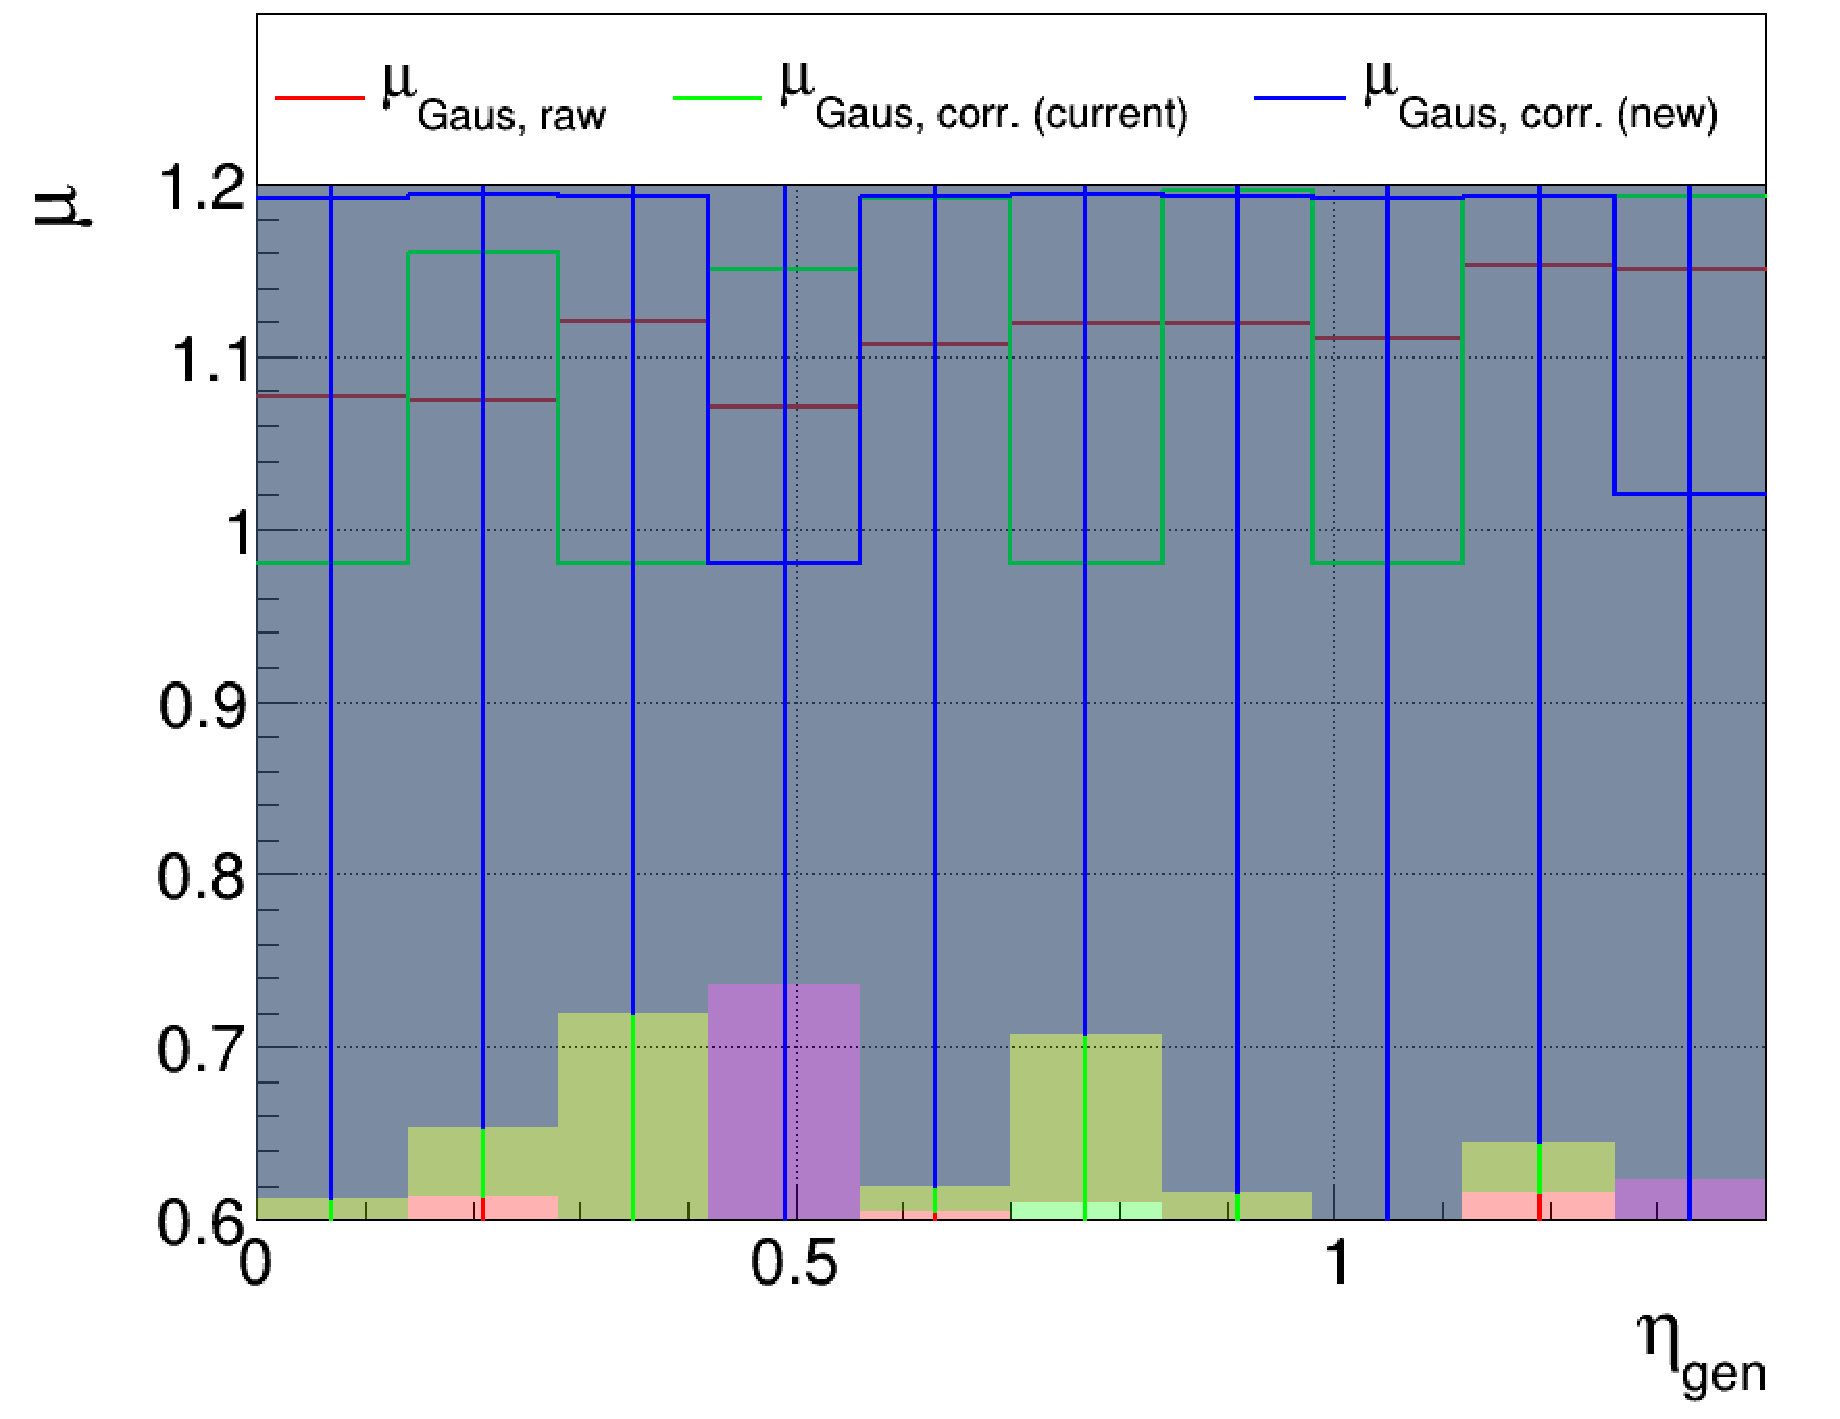
\includegraphics[width=0.495\textwidth]{./plots_pdf/ECAL_plots/plotsNOPU/EB/ZS/pdf/GENETA/EBZS_GENETA_0006_0025_MuOverBins.pdf}
%% 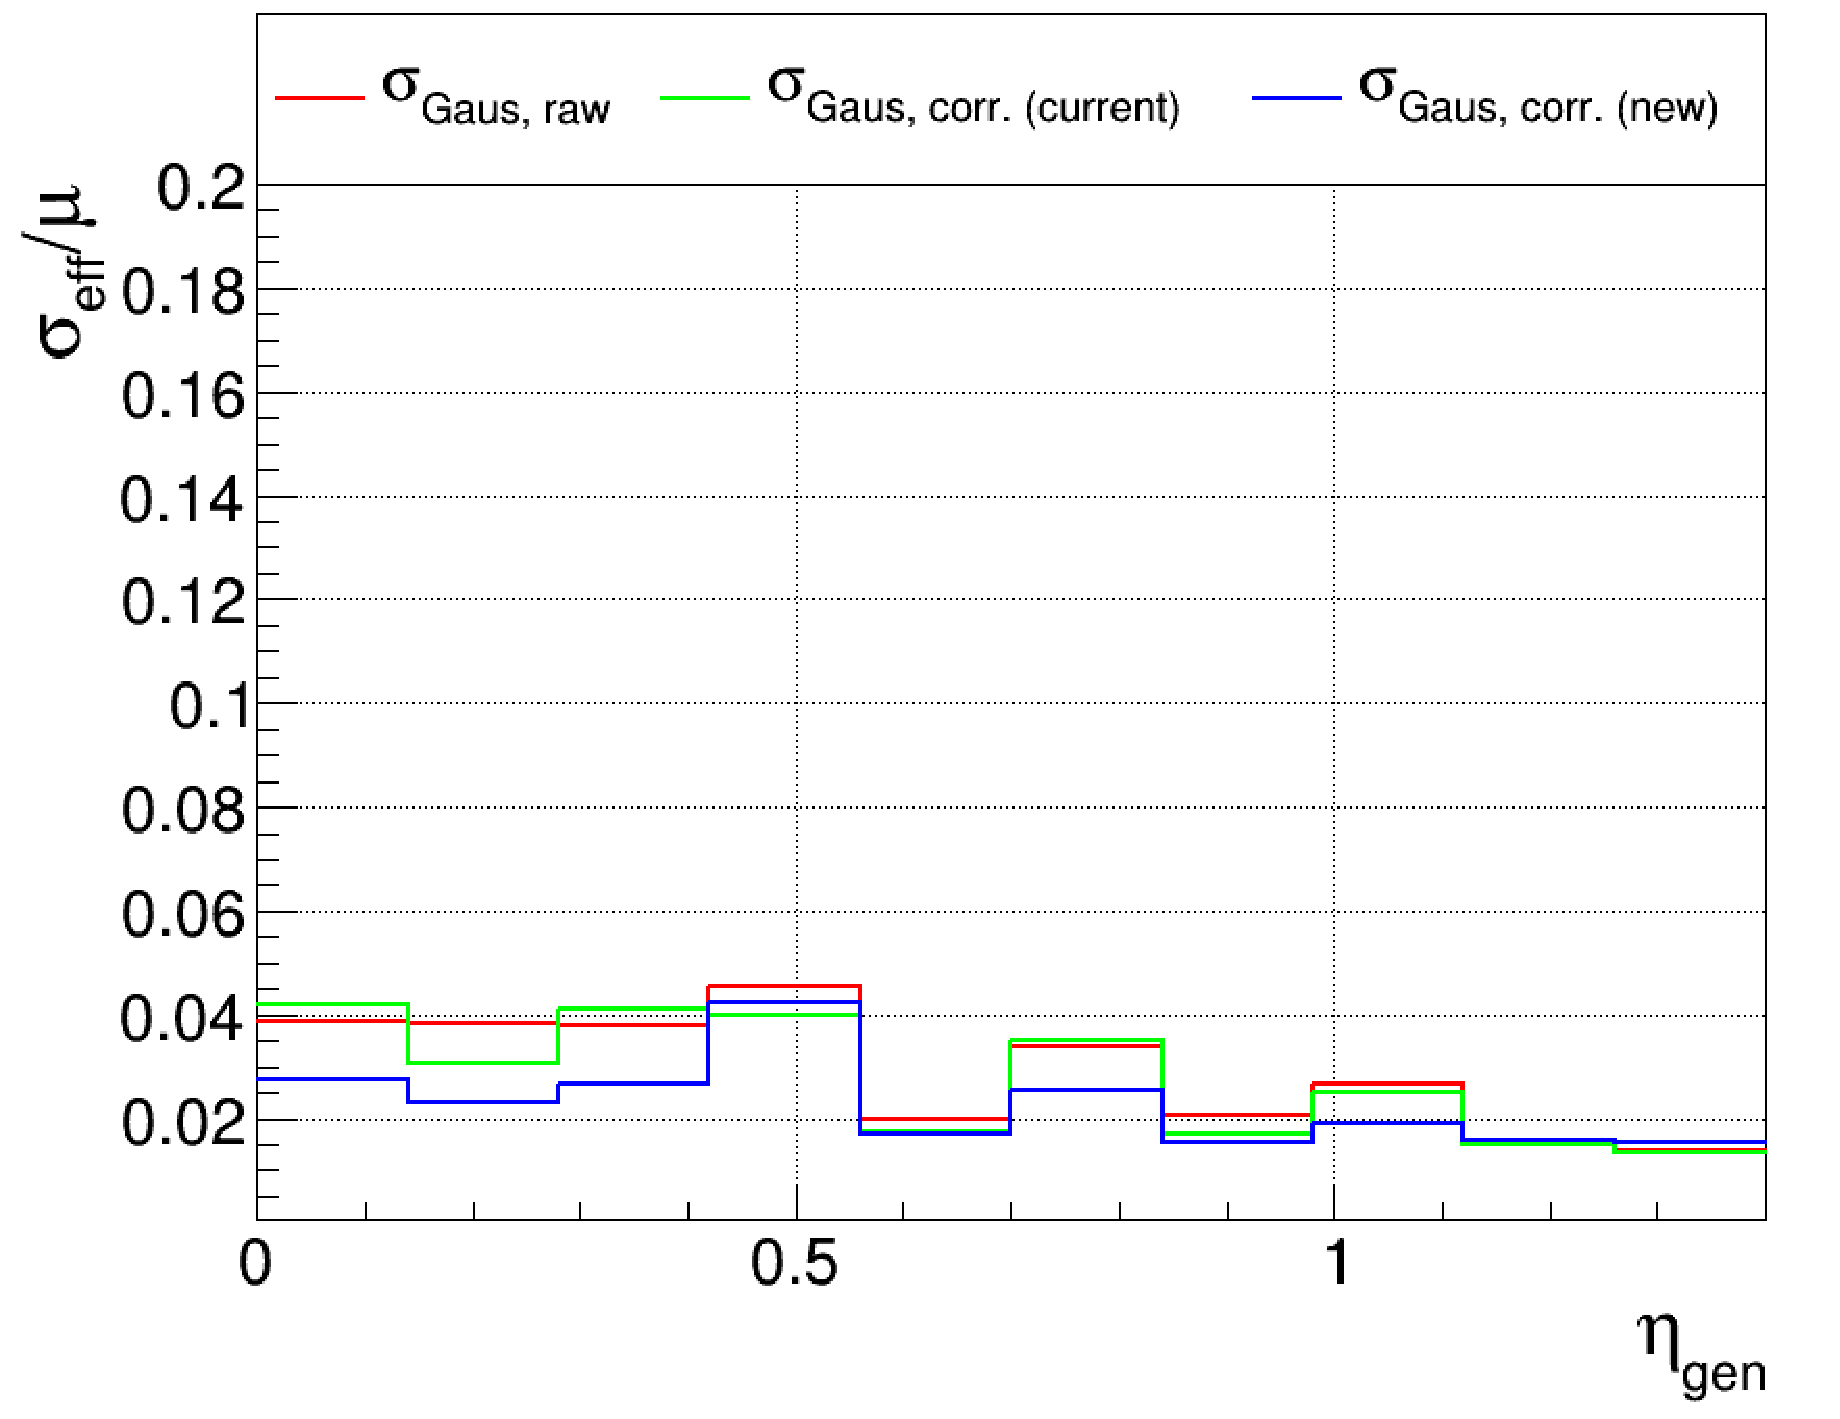
\includegraphics[width=0.495\textwidth]{./plots_pdf/ECAL_plots/plotsNOPU/EB/ZS/pdf/GENETA/EBZS_GENETA_0006_0025_EffSigmaOverBins.pdf}
%% \caption[]{EB - ZS Readout \pt 6-25\GeV}
%% \end{figure}






%\subsubsection{ECAL Endcap}

in EE region:
\begin{figure}
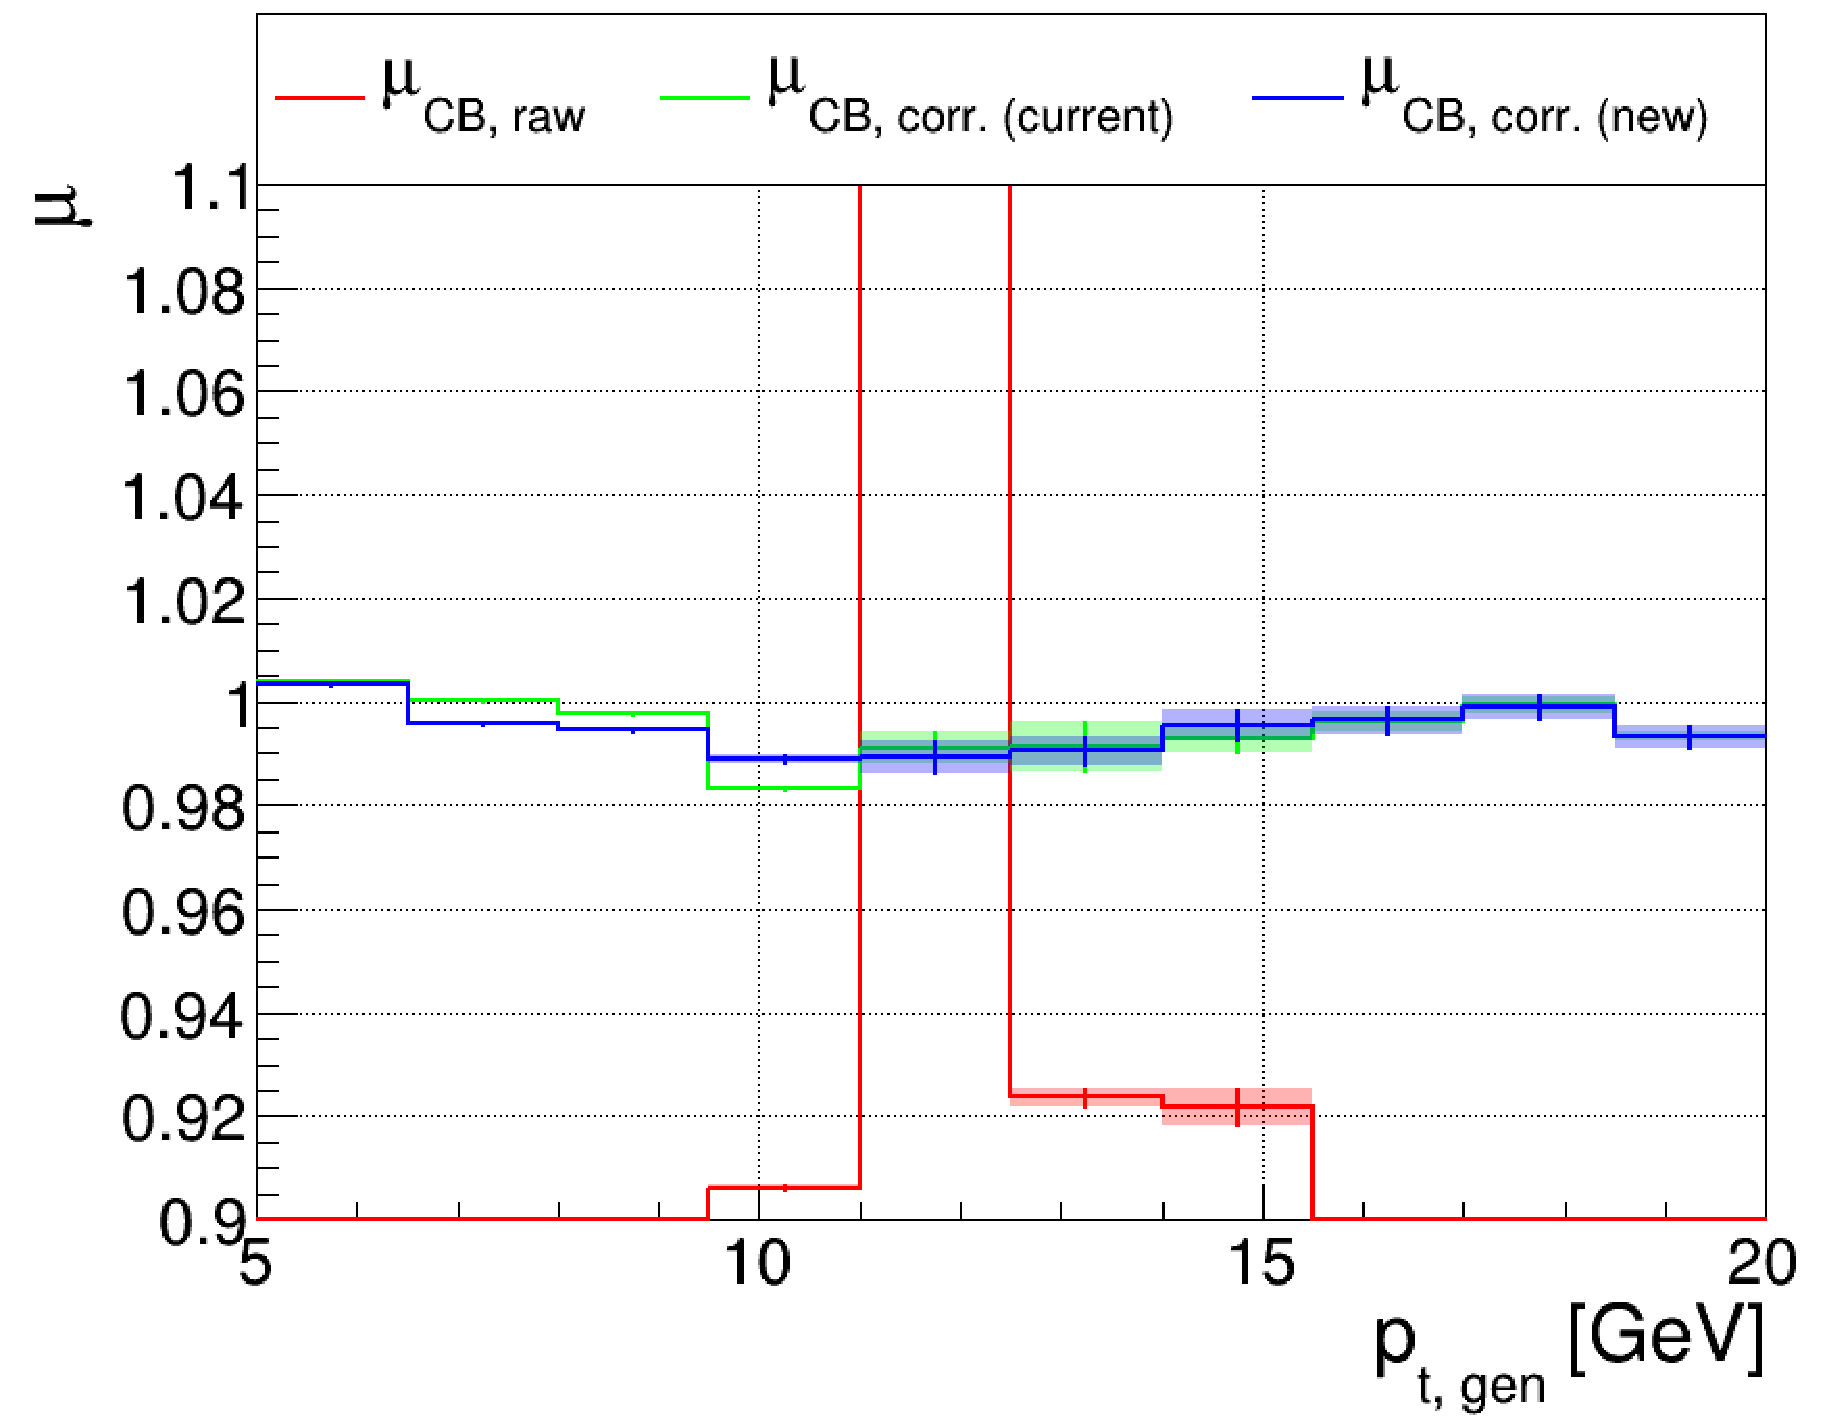
\includegraphics[width=0.495\textwidth]{./plots_pdf/ECAL_plots/plotsNoPU/EE/pdf/FULL/GENPT/EEFULL_GENPT_0005_0020_MuOverBins.pdf}
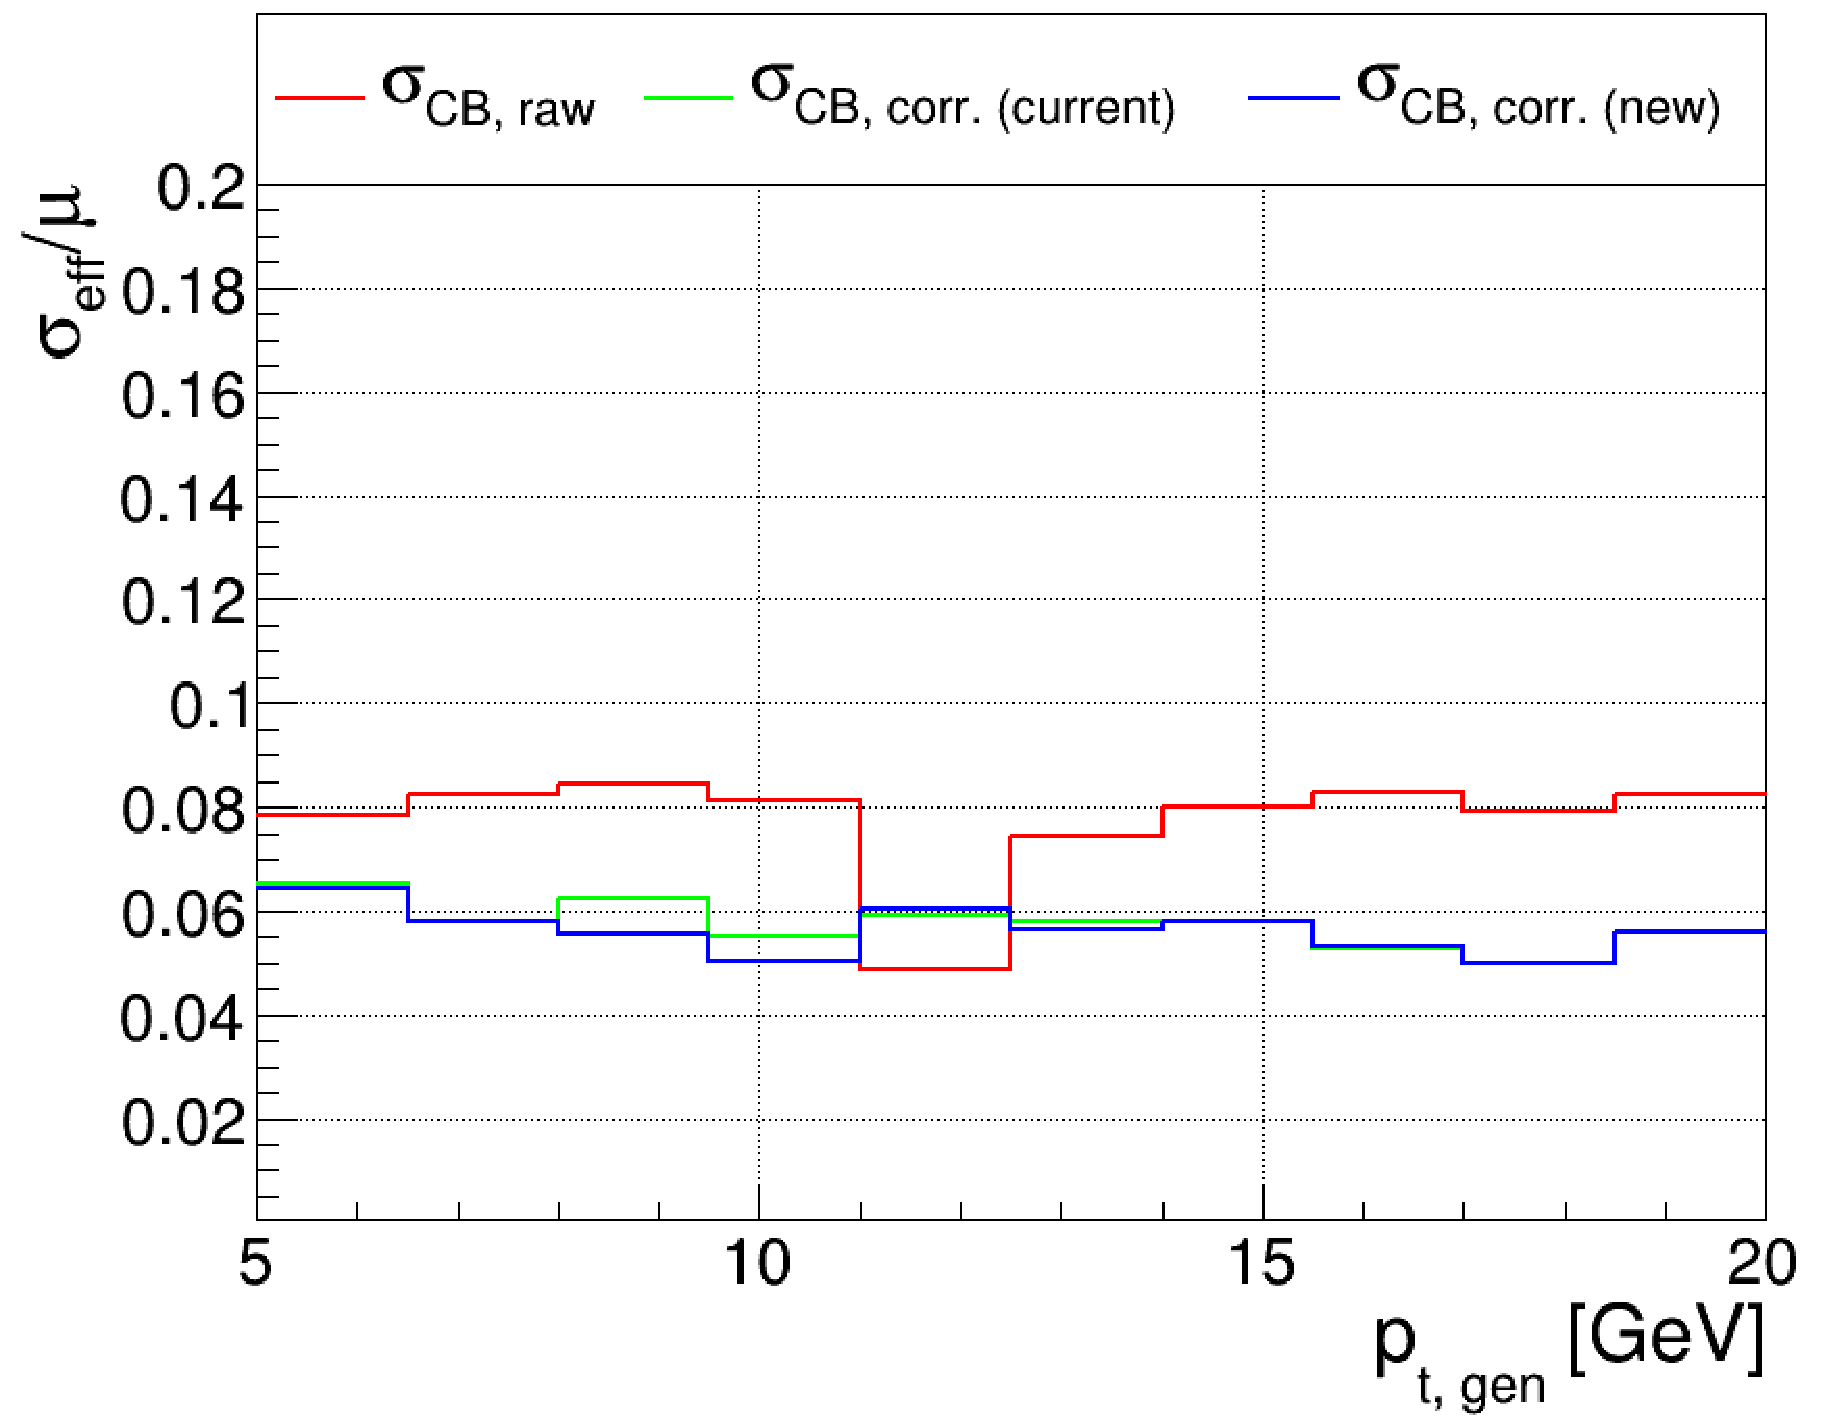
\includegraphics[width=0.495\textwidth]{./plots_pdf/ECAL_plots/plotsNoPU/EE/pdf/FULL/GENPT/EEFULL_GENPT_0005_0020_EffSigmaOverBins.pdf}

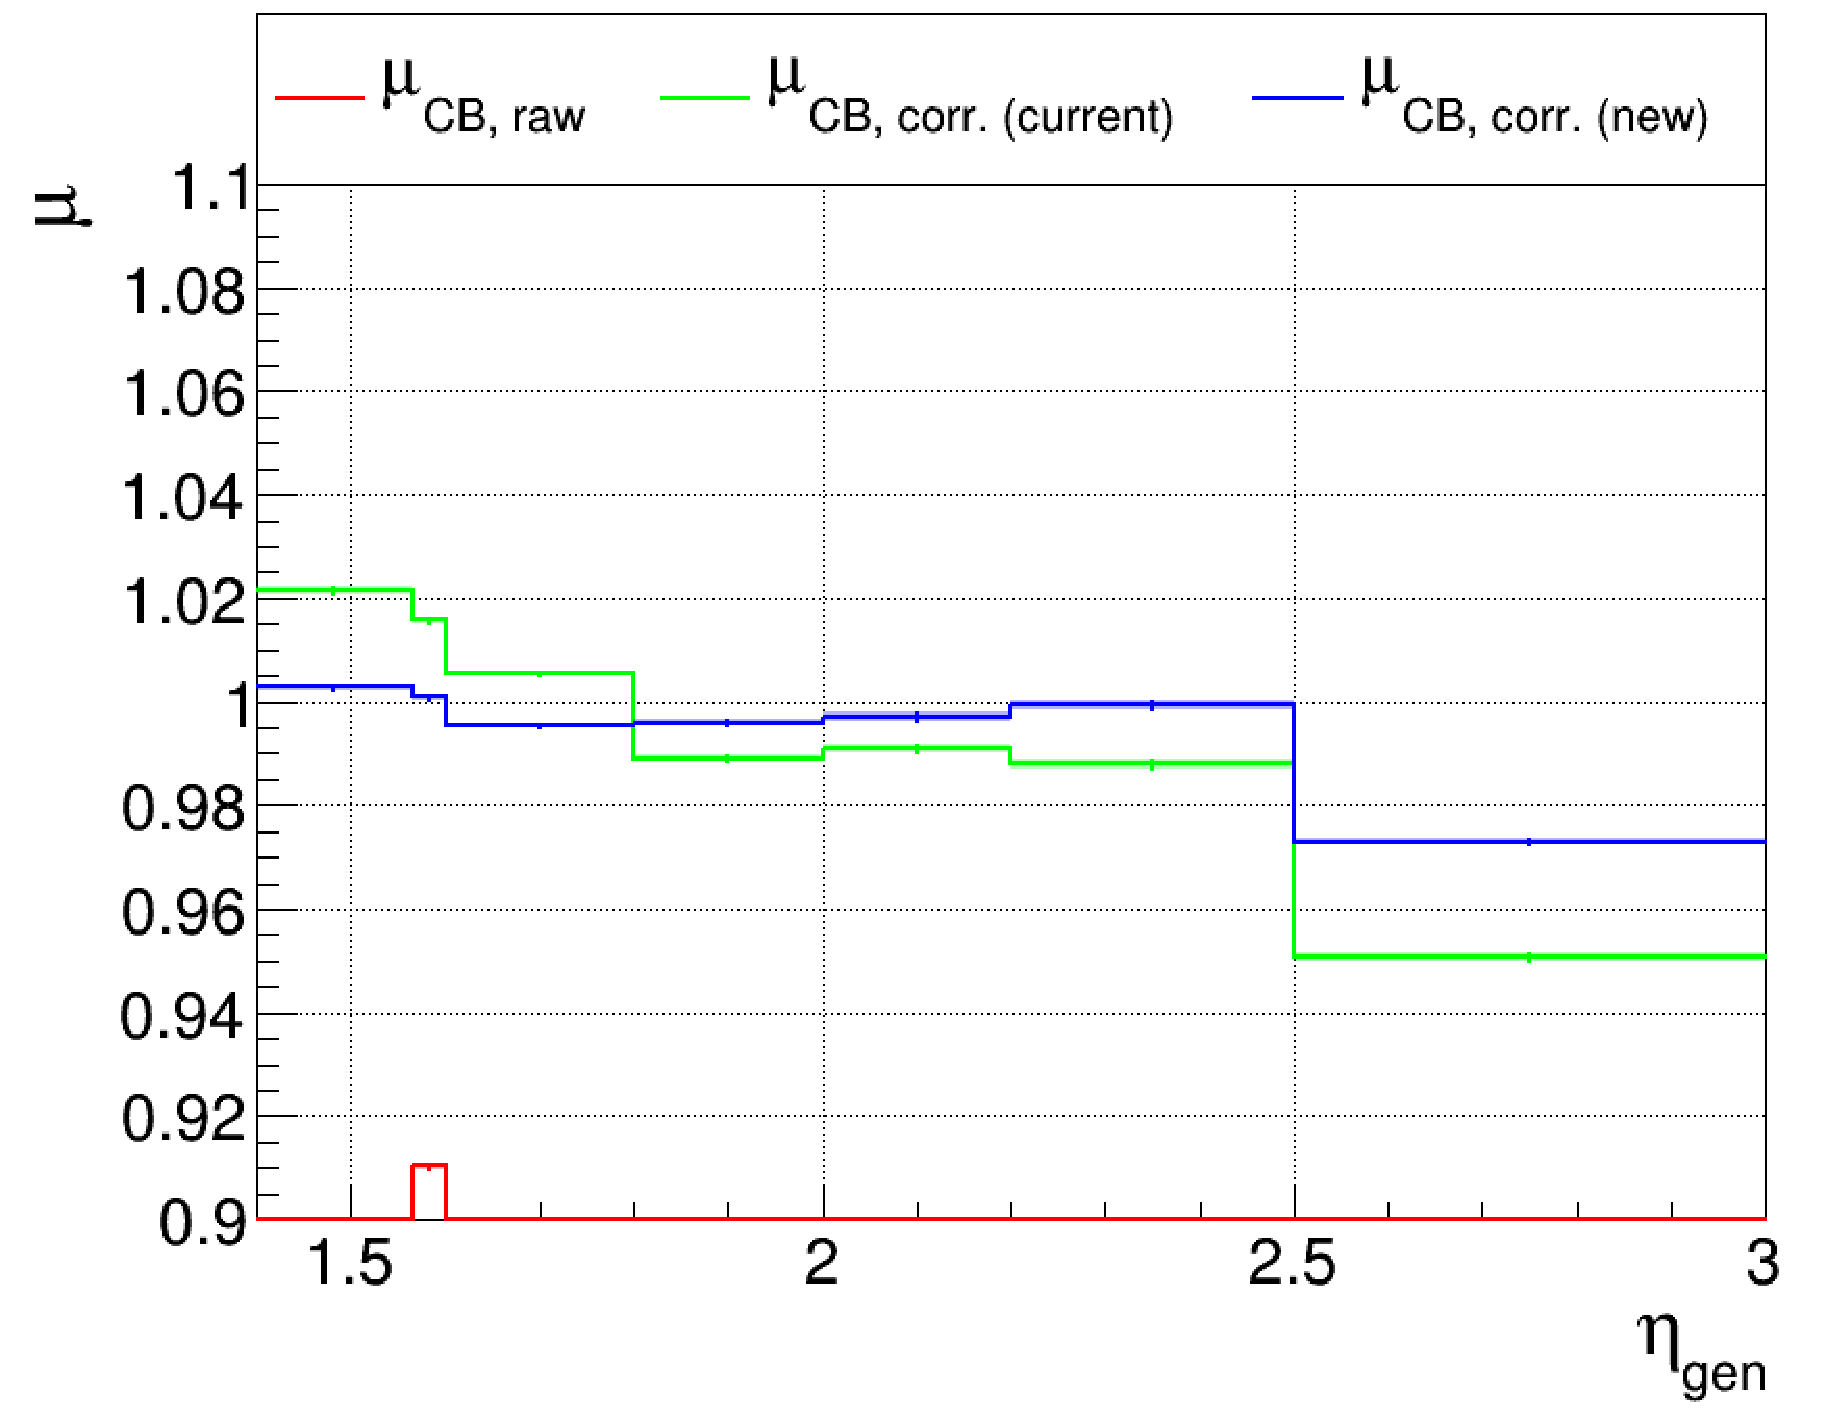
\includegraphics[width=0.495\textwidth]{./plots_pdf/ECAL_plots/plotsNoPU/EE/pdf/FULL/GENETA/EEFULL_GENETA_0005_0020_MuOverBins.pdf}
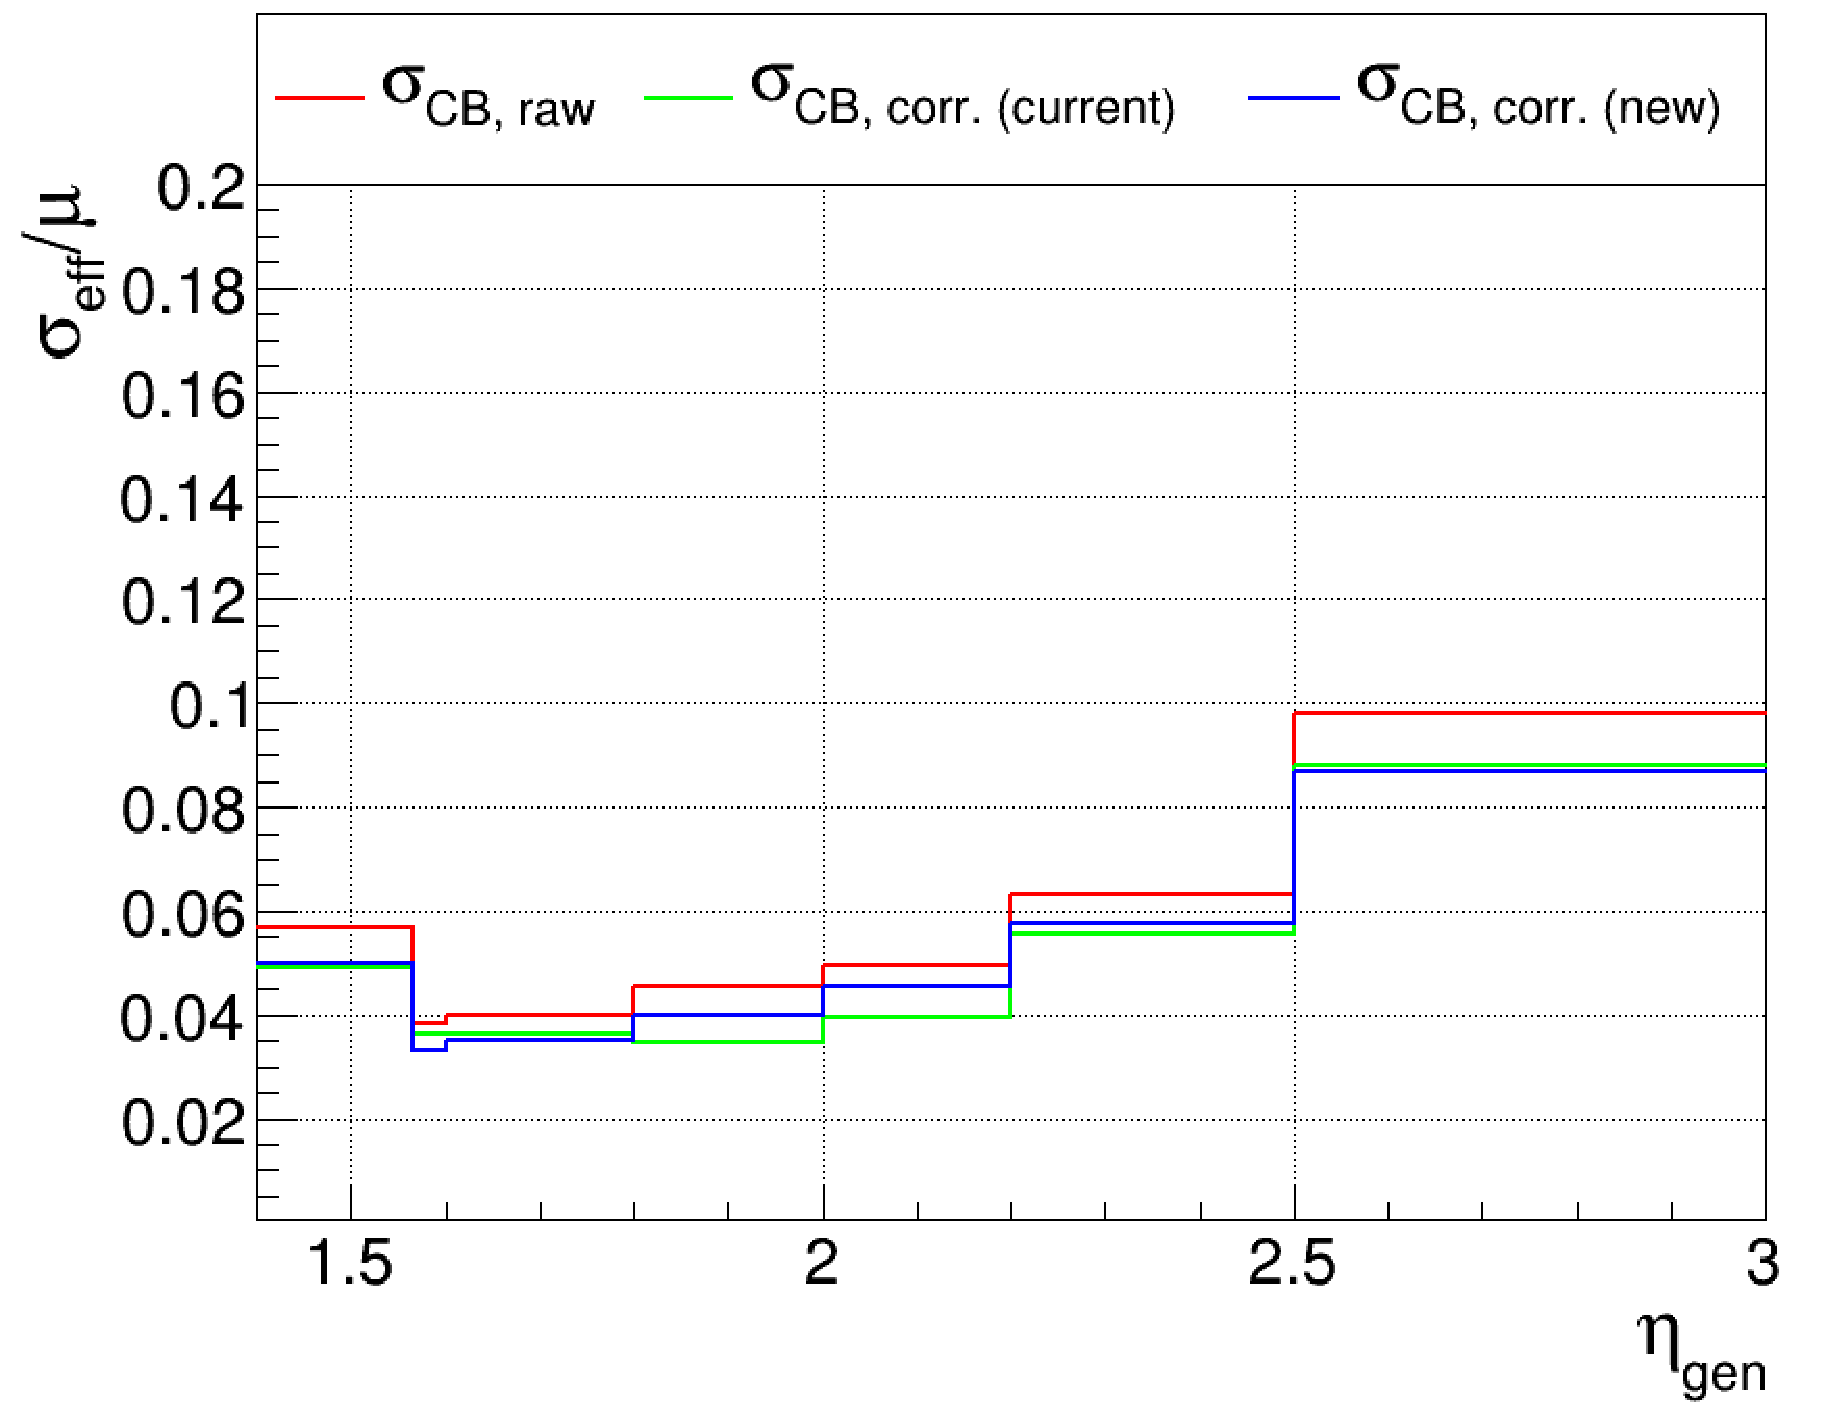
\includegraphics[width=0.495\textwidth]{./plots_pdf/ECAL_plots/plotsNoPU/EE/pdf/FULL/GENETA/EEFULL_GENETA_0005_0020_EffSigmaOverBins.pdf}
\caption{EE - Full Readout \pt 5-20}
%\end{figure}


%\begin{figure}
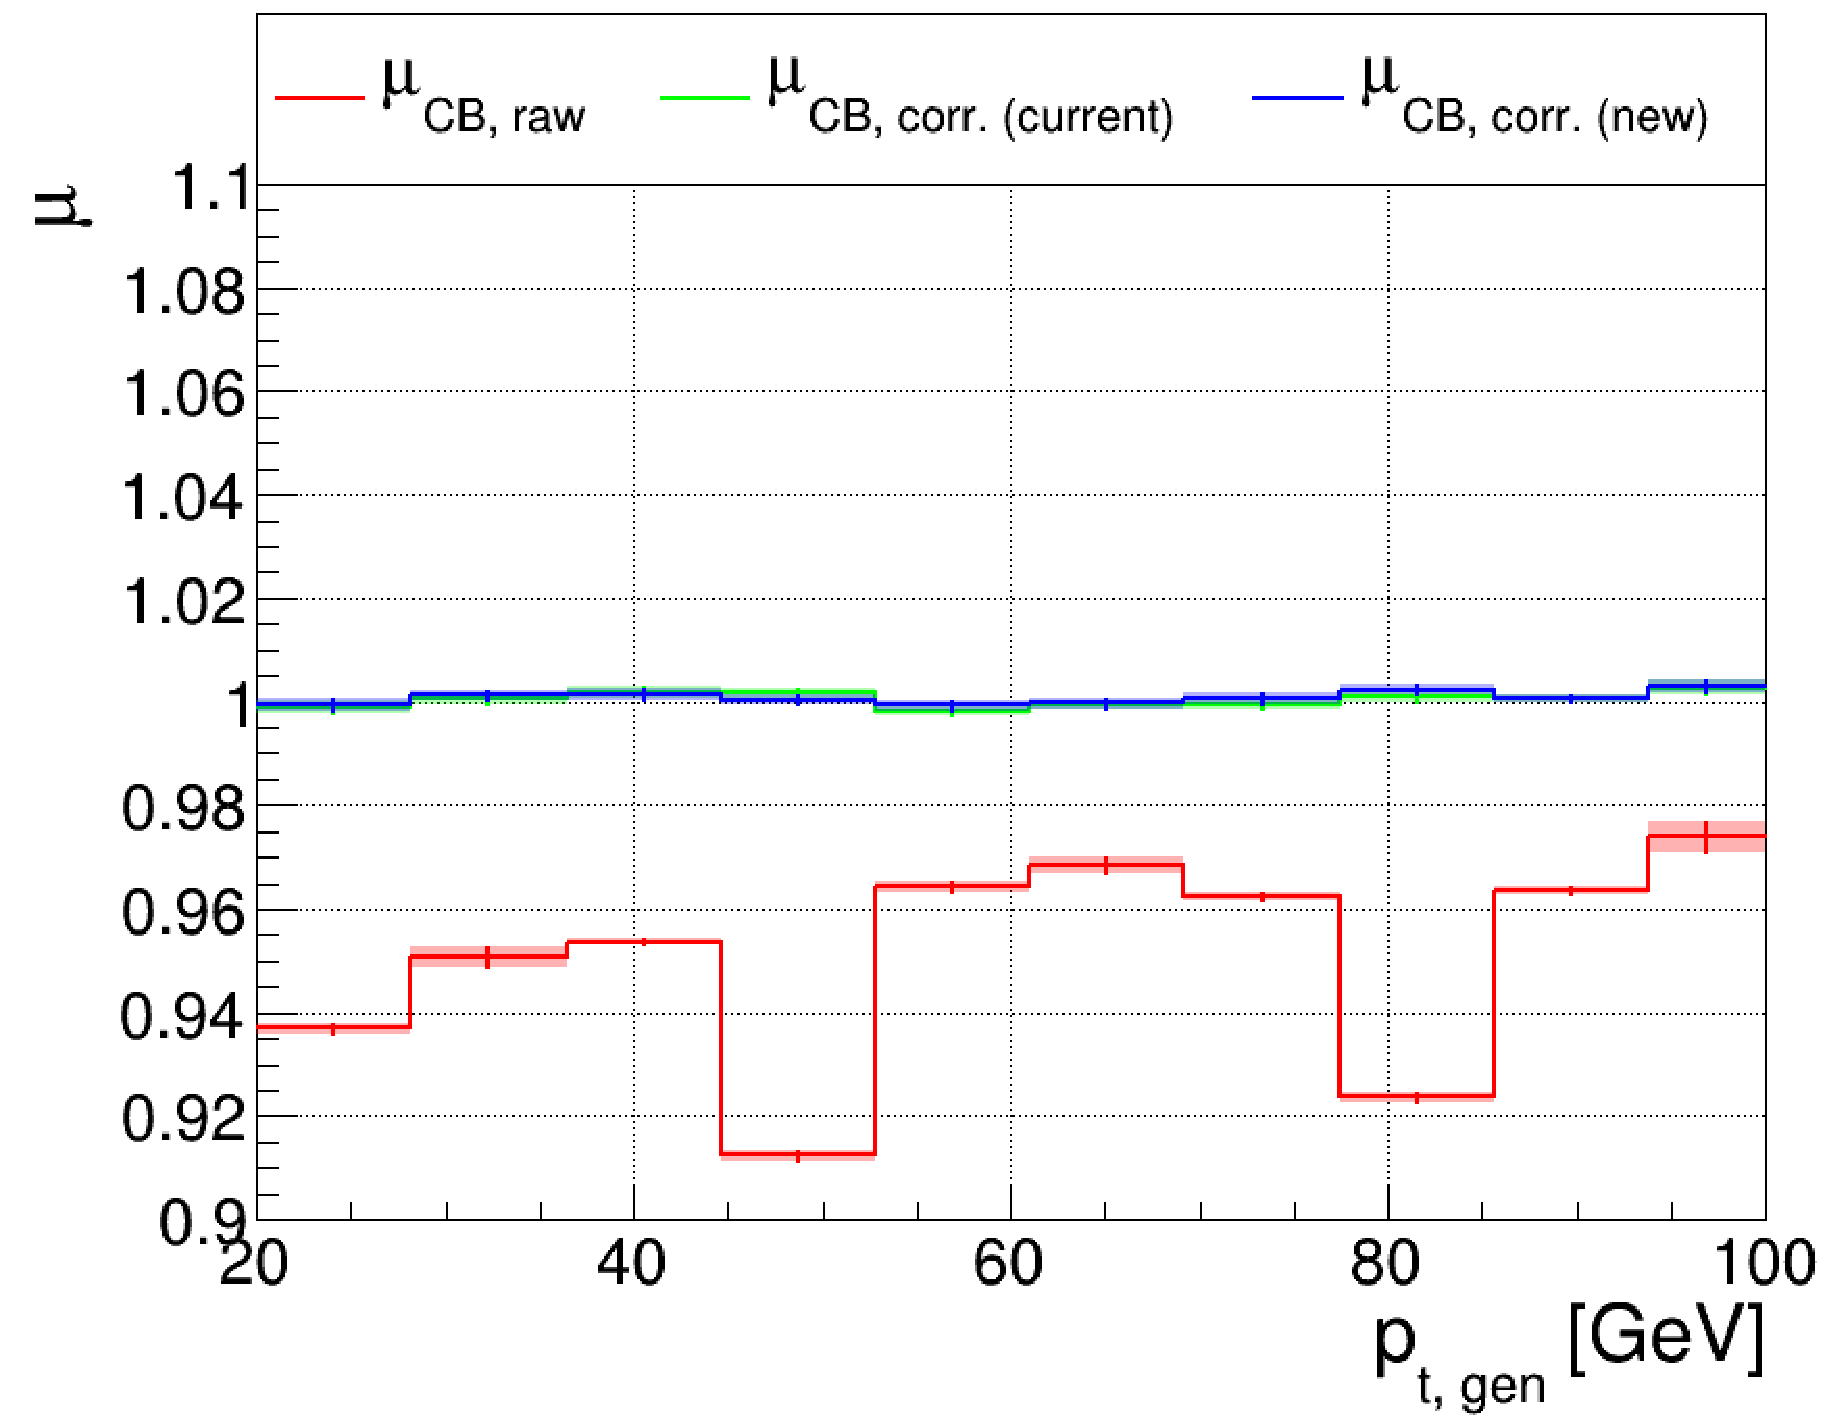
\includegraphics[width=0.495\textwidth]{./plots_pdf/ECAL_plots/plotsNoPU/EE/pdf/FULL/GENPT/EEFULL_GENPT_0020_0100_MuOverBins.pdf}
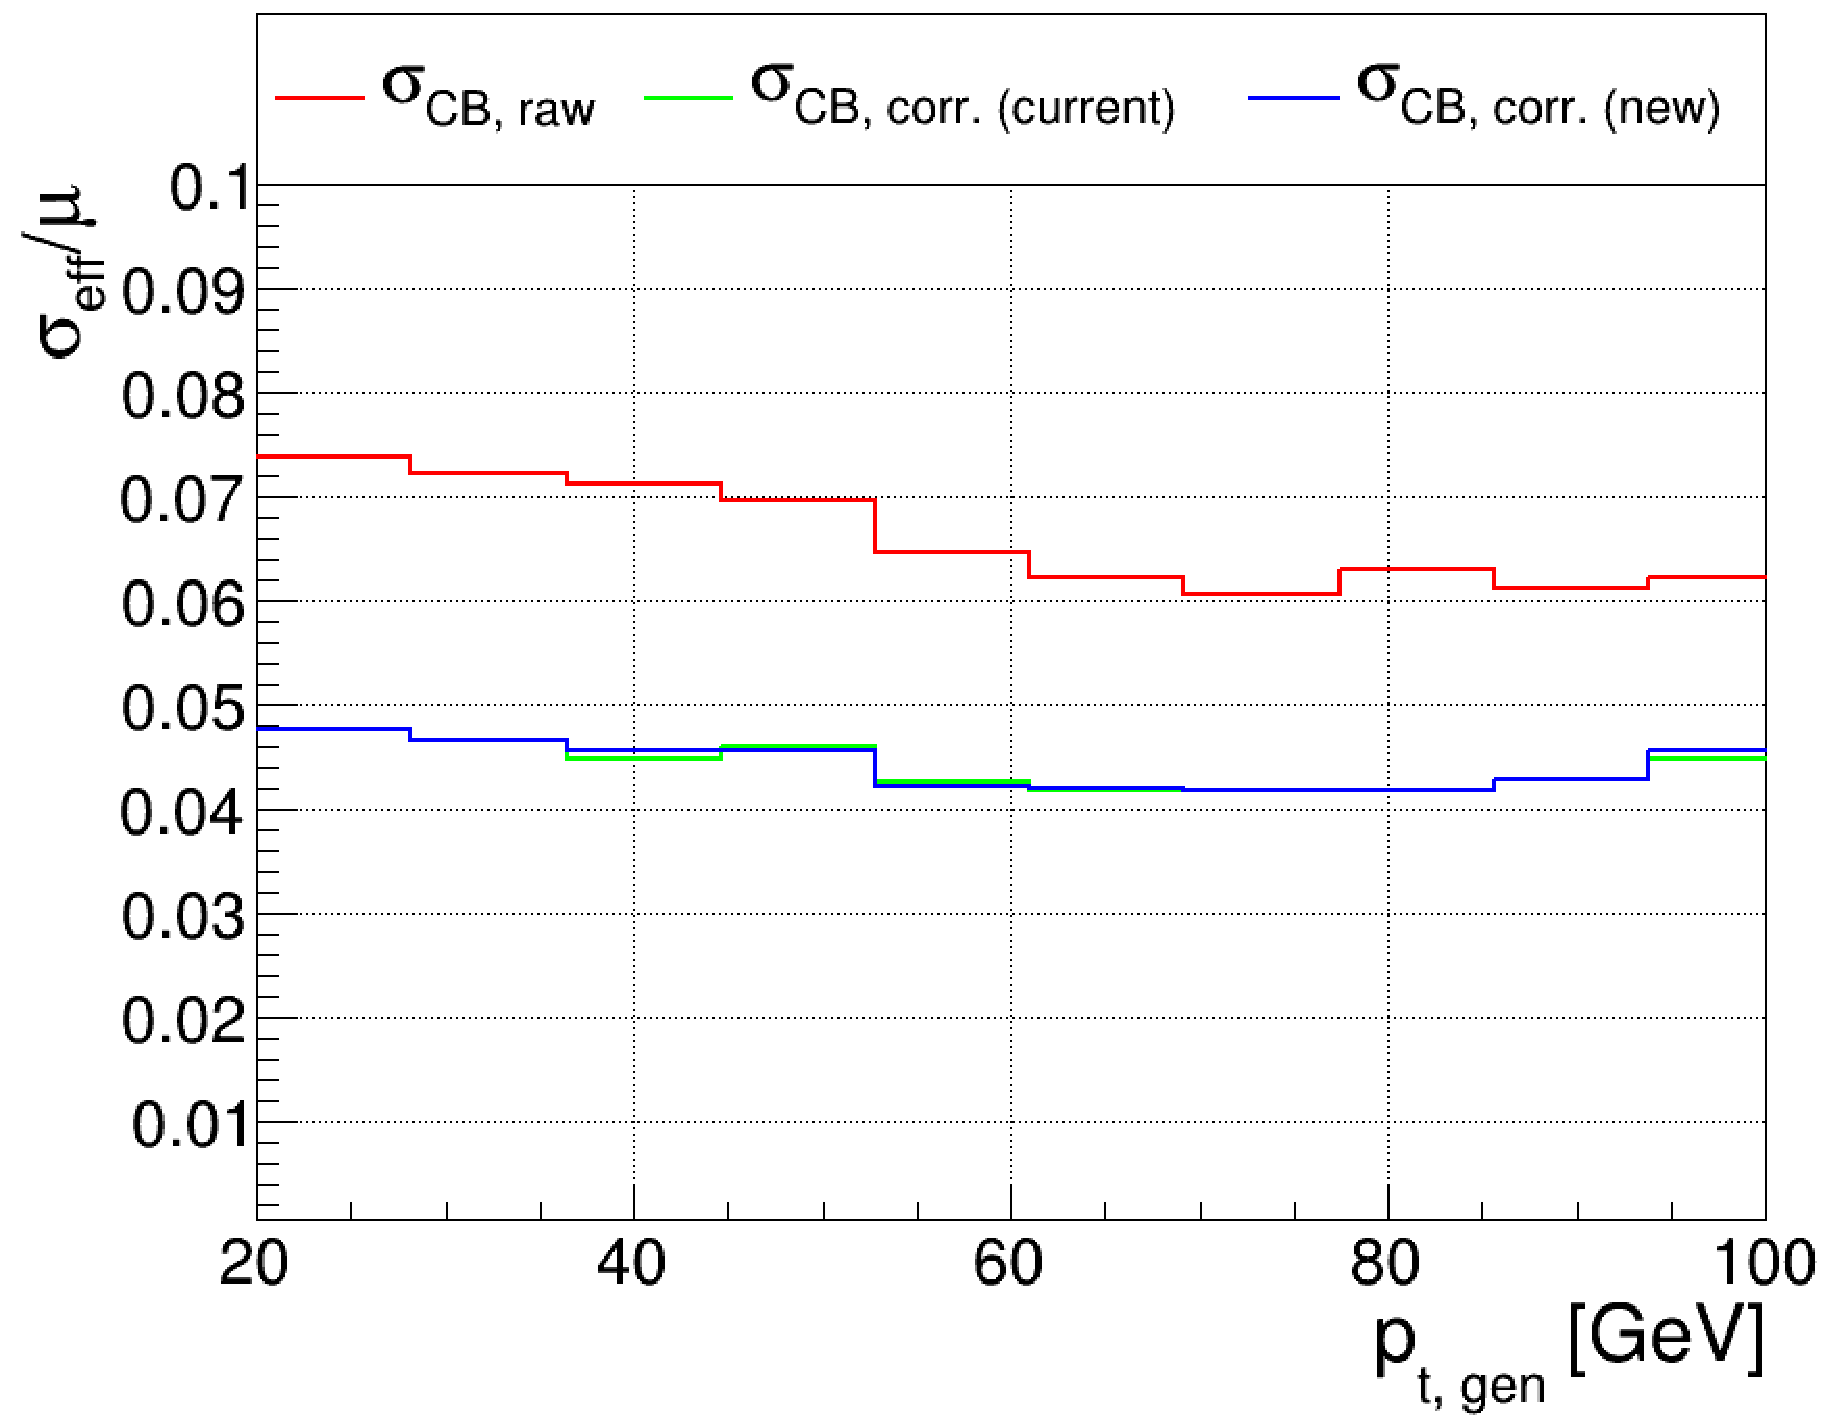
\includegraphics[width=0.495\textwidth]{./plots_pdf/ECAL_plots/plotsNoPU/EE/pdf/FULL/GENPT/EEFULL_GENPT_0020_0100_EffSigmaOverBins.pdf}

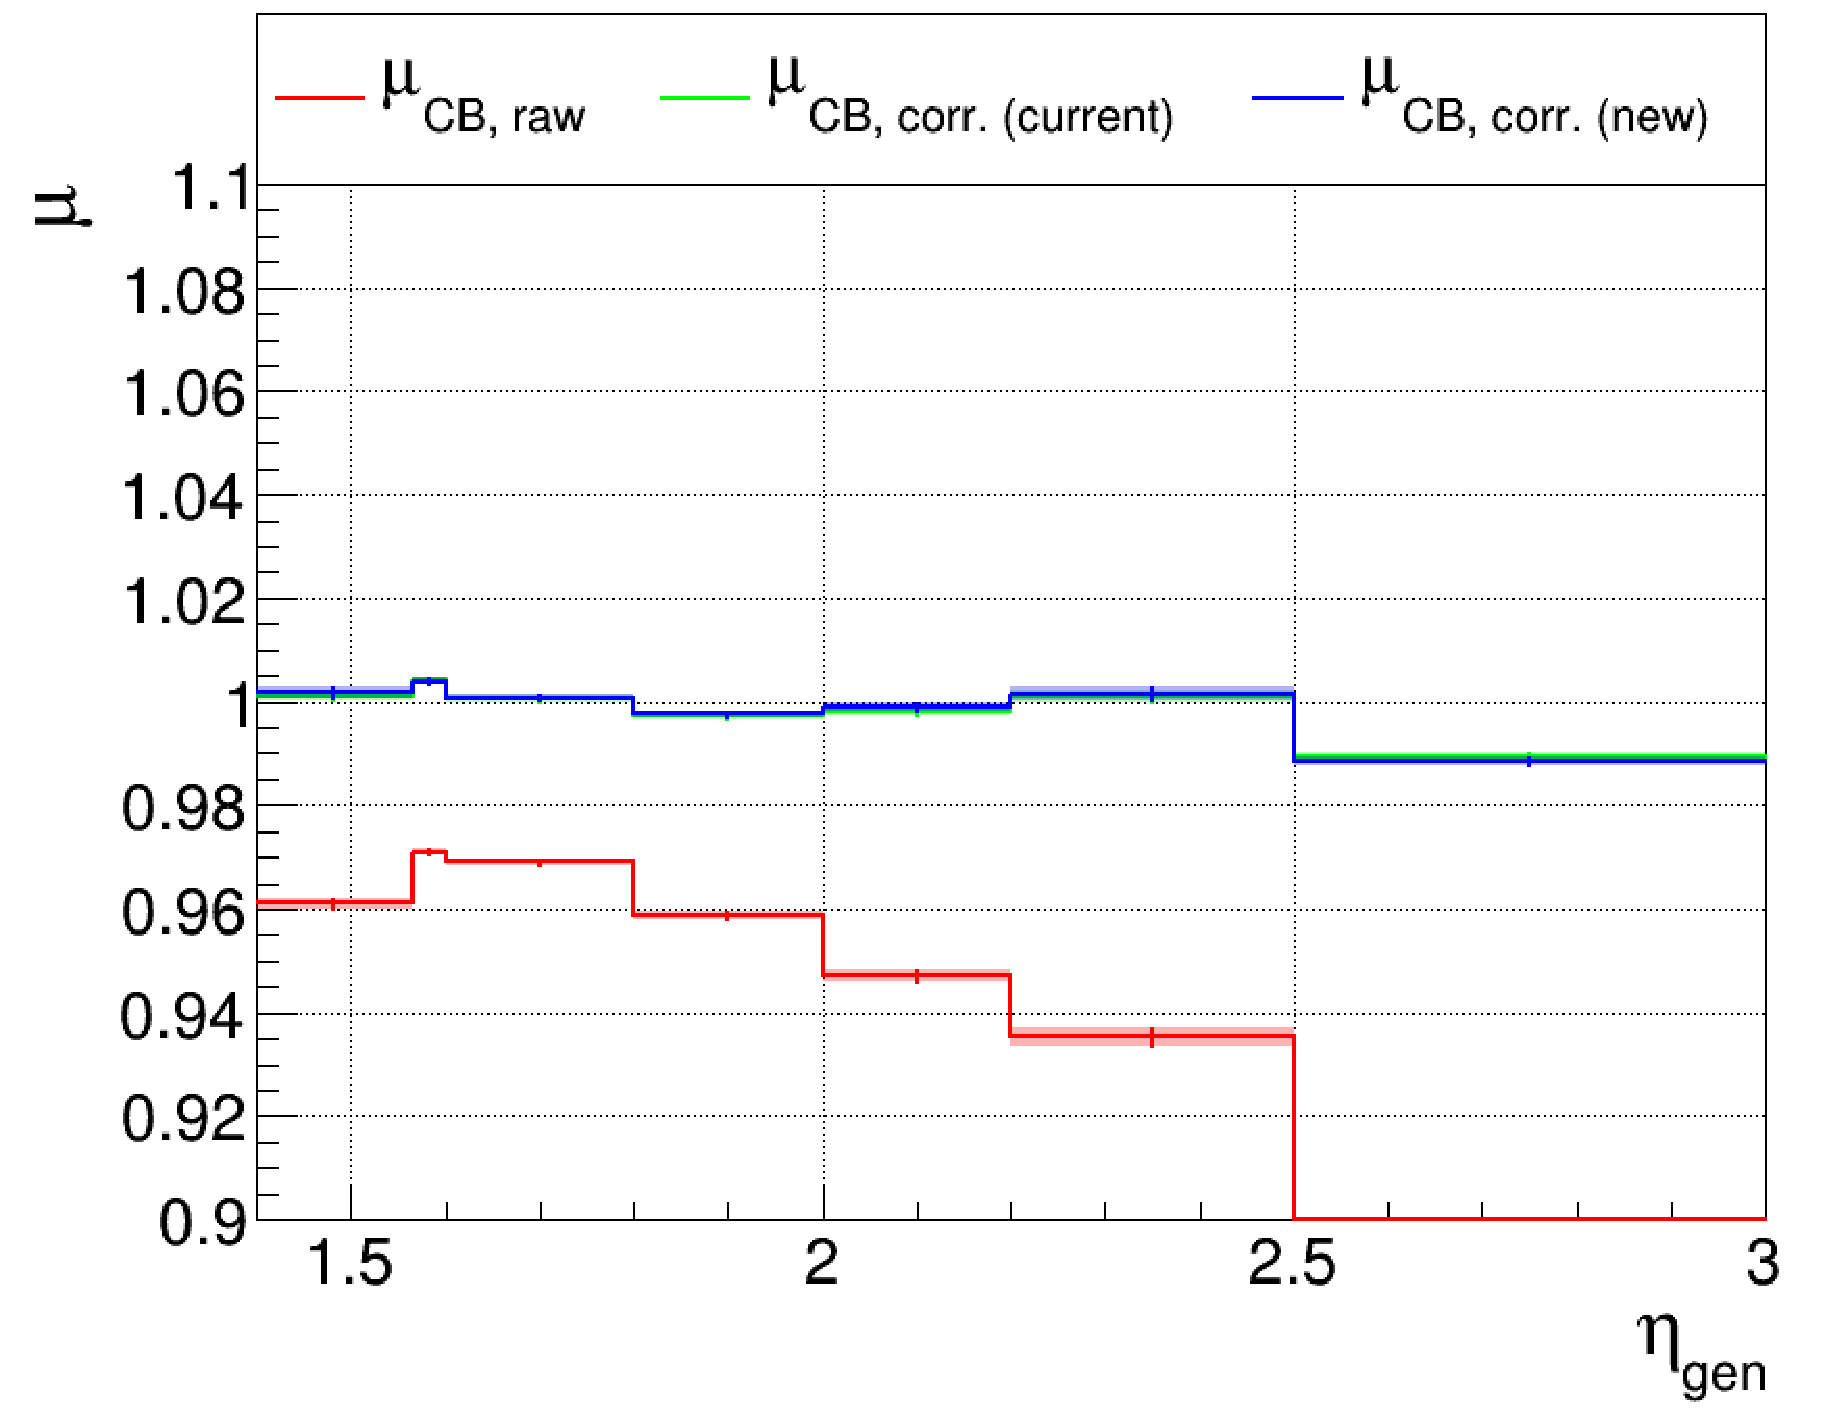
\includegraphics[width=0.495\textwidth]{./plots_pdf/ECAL_plots/plotsNoPU/EE/pdf/FULL/GENETA/EEFULL_GENETA_0020_0100_MuOverBins.pdf}
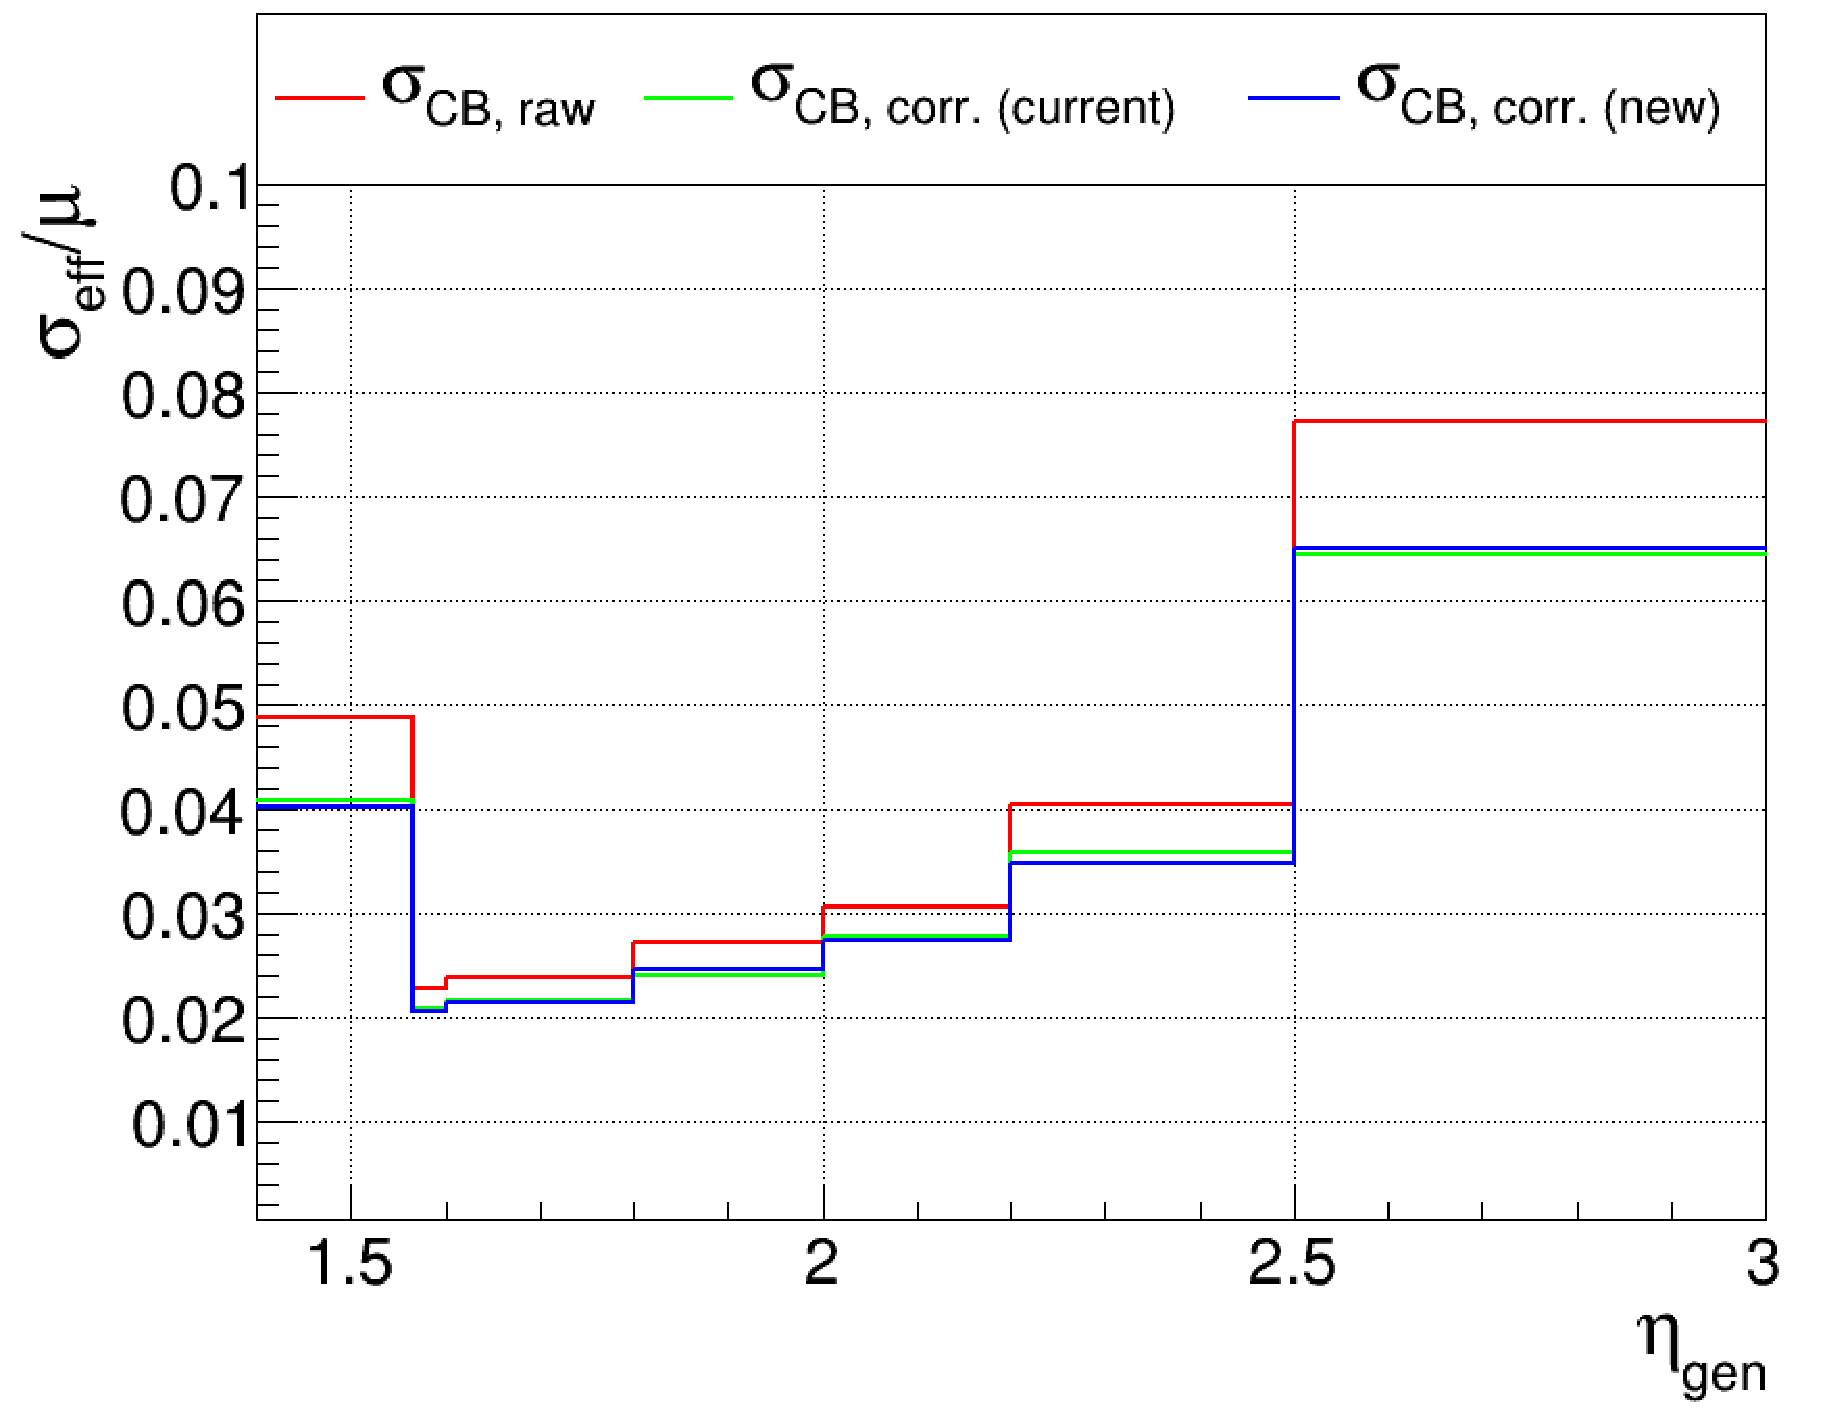
\includegraphics[width=0.495\textwidth]{./plots_pdf/ECAL_plots/plotsNoPU/EE/pdf/FULL/GENETA/EEFULL_GENETA_0020_0100_EffSigmaOverBins.pdf}
\caption{EE - Full Readout \pt 20-100}
\end{figure}


\begin{figure}
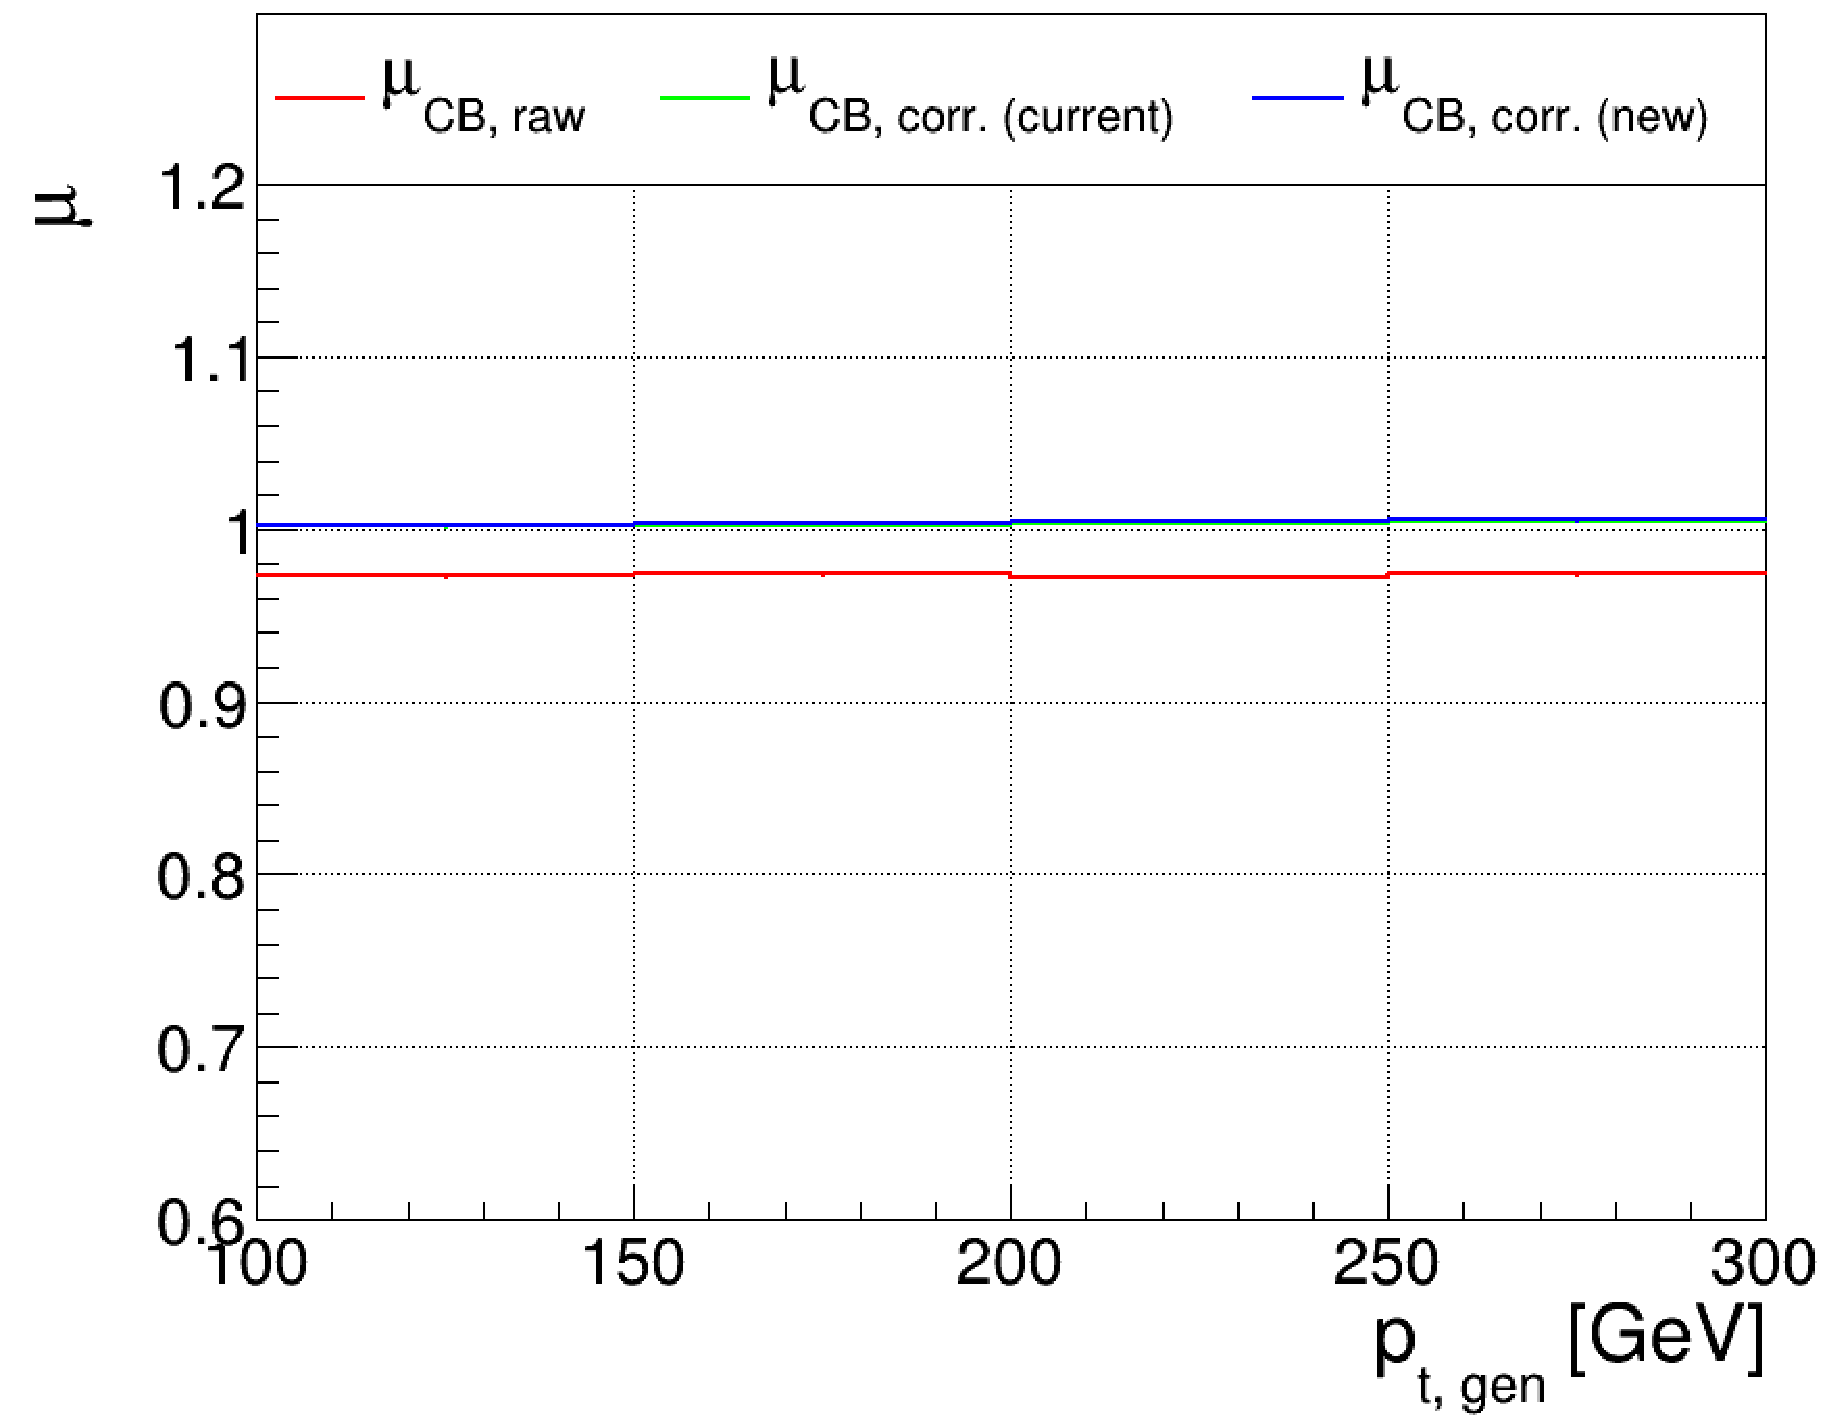
\includegraphics[width=0.495\textwidth]{./plots_pdf/ECAL_plots/plotsNoPU/EE/pdf/FULL/GENPT/EEFULL_GENPT_0100_0300_MuOverBins.pdf}
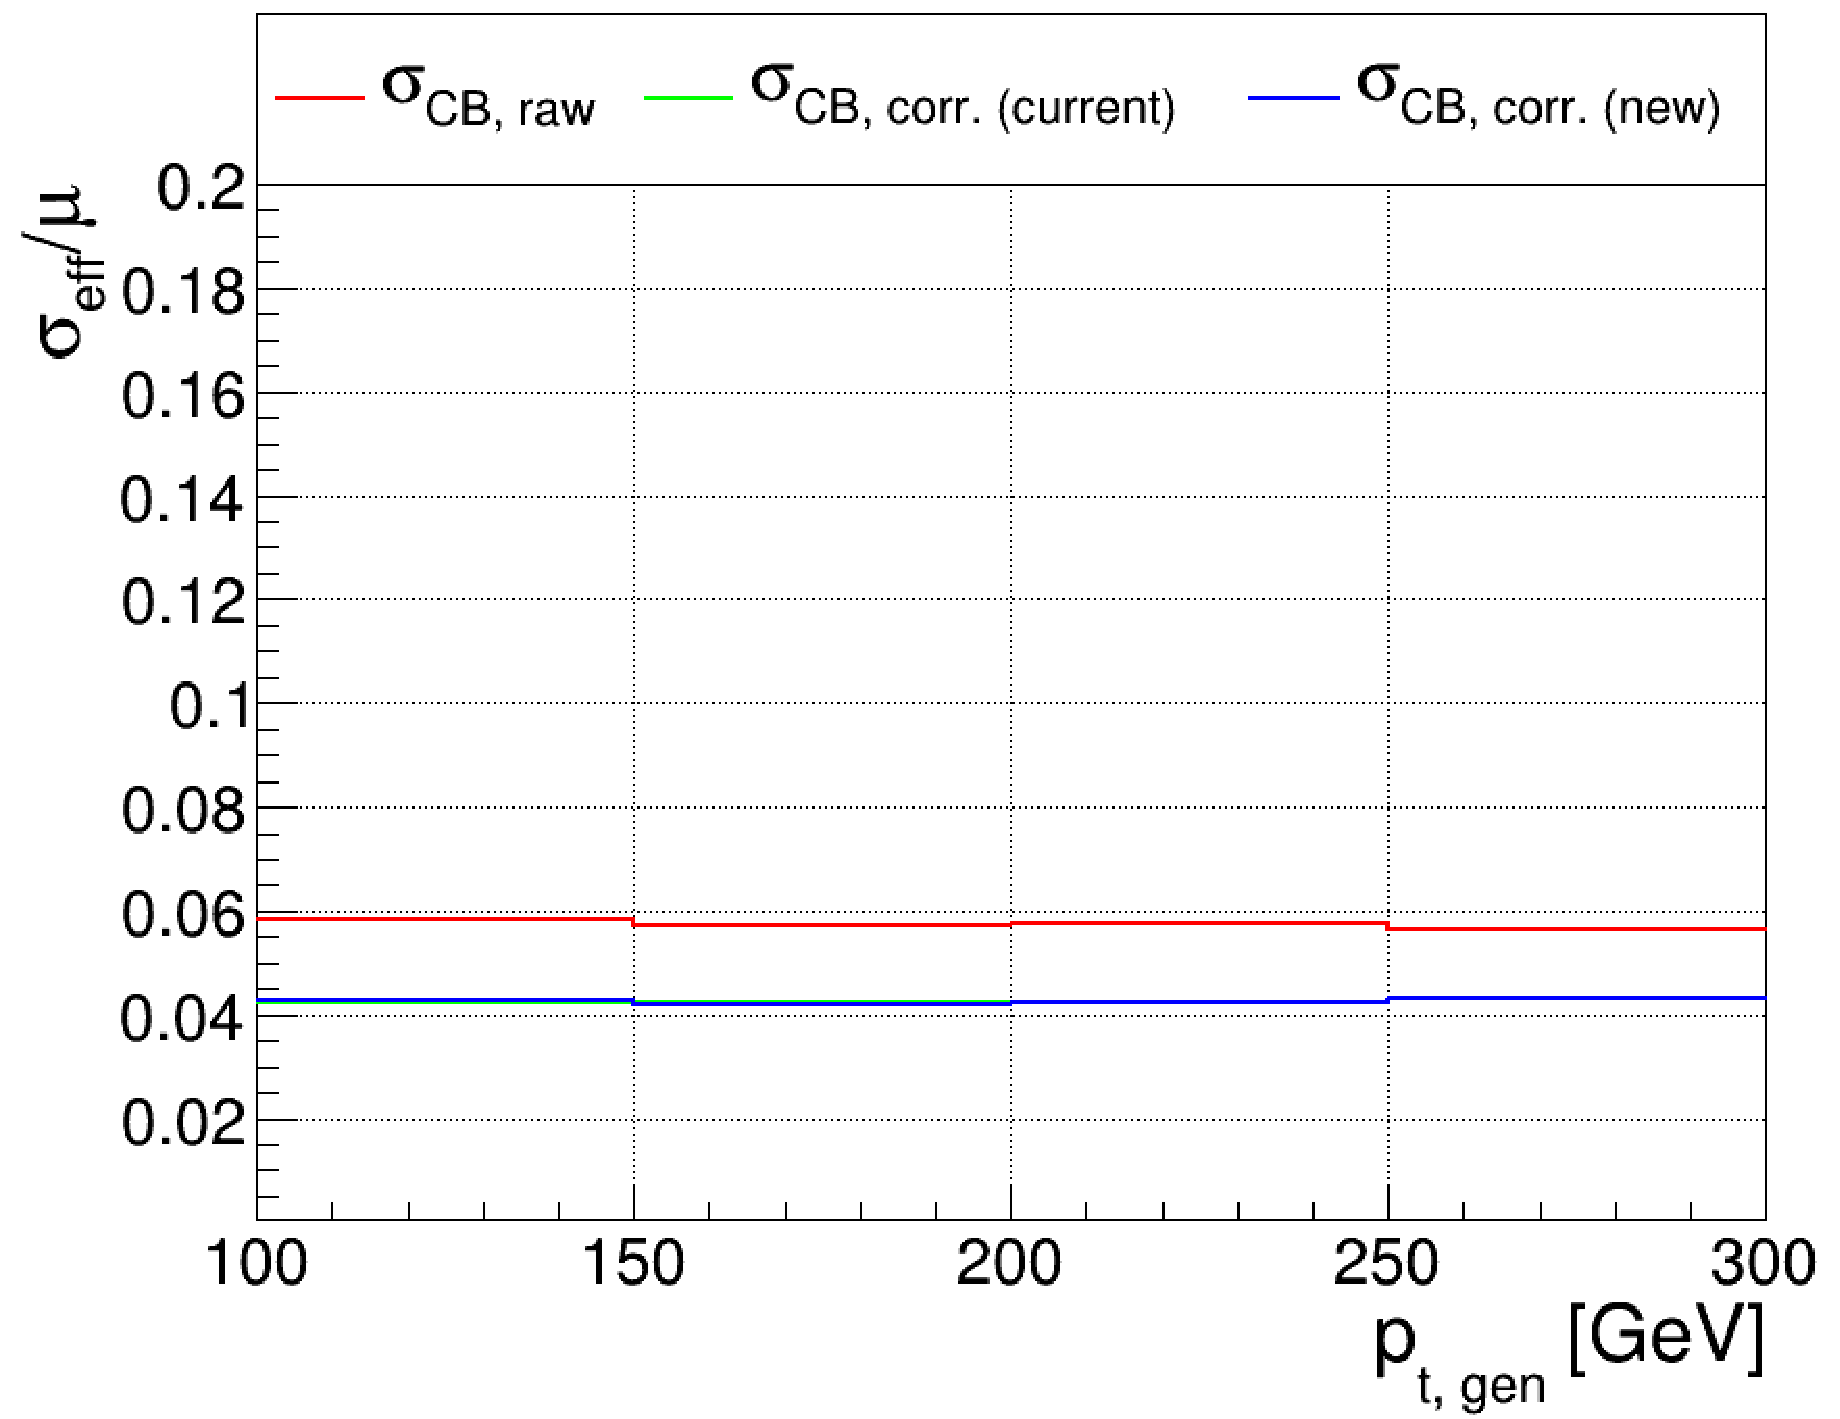
\includegraphics[width=0.495\textwidth]{./plots_pdf/ECAL_plots/plotsNoPU/EE/pdf/FULL/GENPT/EEFULL_GENPT_0100_0300_EffSigmaOverBins.pdf}
%\caption{EE - Full Readout pt 100-300}
%\end{figure}
%\begin{figure}
\includegraphics[width=0.495\textwidth]{./plots_pdf/ECAL_plots/plotsNoPU/EE/pdf/FULL/GENETA/EEFULL_GENETA_0100_0300_MuOverBins.pdf}
\includegraphics[width=0.495\textwidth]{.plots_pdf/ECAL_plots/plotsNoPU/EE/pdf/FULL/GENETA/EEFULL_GENETA_0100_0300_EffSigmaOverBins.pdf}
\caption{EE - Full Readout \pt 100-300}
\end{figure}





\begin{figure}
\includegraphics[width=0.495\textwidth]{./plots_pdf/ECAL_plots/plotsNoPU/EE/pdf/ZS/GENPT/EEZS_GENPT_0000_0006_MuOverBins.pdf}
\includegraphics[width=0.495\textwidth]{./plots_pdf/ECAL_plots/plotsNoPU/EE/pdf/ZS/GENPT/EEZS_GENPT_0000_0006_EffSigmaOverBins.pdf}

\includegraphics[width=0.495\textwidth]{./plots_pdf/ECAL_plots/plotsNoPU/EE/pdf/ZS/GENETA/EEZS_GENETA_0000_0006_MuOverBins.pdf}
\includegraphics[width=0.495\textwidth]{./plots_pdf/ECAL_plots/plotsNoPU/EE/pdf/ZS/GENETA/EEZS_GENETA_0000_0006_EffSigmaOverBins.pdf}
\caption[$\mu$ ($\sigma_\mathrm{eff}$) vs \pt of PF ECAL cluster - EE ZS readout NoPU scenario]{Mean response (resolution) defined by Raw PF ECAL clusters (red), the calibration derived earlier in Ru\
n3 based on 126X (green), and the new correction from 2024 simulation sample based on 133X (blue).\pt 0--6\GeV in EE region ZS Readout NOPU scenario.}
\end{figure}

%% %\begin{figure}
%% \includegraphics[width=0.495\textwidth]{./plots_pdf/ECAL_plots/plotsNoPU/EE/pdf/ZS/GENPT/EEZS_GENPT_0006_0025_MuOverBins.pdf}
%% \includegraphics[width=0.495\textwidth]{./plots_pdf/ECAL_plots/plotsNoPU/EE/pdf/ZS/GENPT/EEZS_GENPT_0006_0025_EffSigmaOverBins.pdf}
%% %\caption{EE - ZS Readout pt 6-25}
%% %\end{figure}
%% %\begin{figure}
%% \includegraphics[width=0.495\textwidth]{./plots_pdf/ECAL_plots/plotsNoPU/EE/pdf/ZS/GENETA/EEZS_GENETA_0006_0025_MuOverBins.pdf}
%% %\includegraphics[width=0.495\textwidth]{./ECAL_plots/plotsNoPU/EE/pdf/ZS/GENETA/EEZS_GENETA_0006_0025_EffSigmaOverBins.pdf}
%% \caption{EE - ZS Readout \pt 6-25}
%% \end{figure}




\begin{figure}
\includegraphics[width=0.495\textwidth]{./plots_pdf/ECAL_plots/plotsPU/EE/FULL/pdf/GENPT/EEFULL_GENPT_0005_0020_MuOverBins.pdf}
\includegraphics[width=0.495\textwidth]{./plots_pdf/ECAL_plots/plotsPU/EE/FULL/pdf/GENPT/EEFULL_GENPT_0005_0020_EffSigmaOverBins.pdf}
\includegraphics[width=0.495\textwidth]{./plots_pdf/ECAL_plots/plotsPU/EE/FULL/pdf/GENPT/EEFULL_GENPT_0020_0100_MuOverBins.pdf}
\includegraphics[width=0.495\textwidth]{./plots_pdf/ECAL_plots/plotsPU/EE/FULL/pdf/GENPT/EEFULL_GENPT_0020_0100_EffSigmaOverBins.pdf}
\includegraphics[width=0.495\textwidth]{./plots_pdf/ECAL_plots/plotsPU/EE/FULL/pdf/GENPT/EEFULL_GENPT_0100_0300_MuOverBins.pdf}
\includegraphics[width=0.495\textwidth]{./plots_pdf/ECAL_plots/plotsPU/EE/FULL/pdf/GENPT/EEFULL_GENPT_0100_0300_EffSigmaOverBins.pdf}

\caption [$\mu$ ($\sigma_\mathrm{eff}$) vs \pt of PF ECAL cluster - EE full readout PU scenario]{Mean response (resolution) defined by Raw PF ECAL clusters (red), the calibration derived earlier in Ru\
n3 based on 126X (green), and the new correction from 2024 simulation sample based on 133X (blue). (top) low \pt, (middle) mid \pt, (bottom) high \pt in EE region full readout PU scenario.}
\label{fig:PU_EEFULL_pt}
\end{figure}


\begin{figure}
\includegraphics[width=0.495\textwidth]{./plots_pdf/ECAL_plots/plotsPU/EE/FULL/pdf/GENETA/EEFULL_GENETA_0005_0020_MuOverBins.pdf}
\includegraphics[width=0.495\textwidth]{./plots_pdf/ECAL_plots/plotsPU/EE/FULL/pdf/GENETA/EEFULL_GENETA_0005_0020_EffSigmaOverBins.pdf}
\includegraphics[width=0.495\textwidth]{./plots_pdf/ECAL_plots/plotsPU/EE/FULL/pdf/GENETA/EEFULL_GENETA_0020_0100_MuOverBins.pdf}
\includegraphics[width=0.495\textwidth]{./plots_pdf/ECAL_plots/plotsPU/EE/FULL/pdf/GENETA/EEFULL_GENETA_0020_0100_EffSigmaOverBins.pdf}
\includegraphics[width=0.495\textwidth]{./plots_pdf/ECAL_plots/plotsPU/EE/FULL/pdf/GENETA/EEFULL_GENETA_0100_0300_MuOverBins.pdf}
\includegraphics[width=0.495\textwidth]{./plots_pdf/ECAL_plots/plotsPU/EE/FULL/pdf/GENETA/EEFULL_GENETA_0100_0300_EffSigmaOverBins.pdf}


\caption [$\mu$ ($\sigma_\mathrm{eff}$) vs $\eta$ of PF ECAL cluster - EE Full readout PU scenario]{Mean response (resolution) defined by Raw PF ECAL clusters (red), the calibration derived earlier in\
 Run3 based on 126X (green), and the new correction from 2024 simulation sample based on 133X (blue). (top) low $\eta$, (middle) mid $\eta$, (bottom) high $\eta$ in EE region Full readout PU scenario.}
\label{fig:PU_EEFULL_eta}
\end{figure}

\begin{figure}
\includegraphics[width=0.495\textwidth]{./plots_pdf/ECAL_plots/plotsPU/EE/ZS/pdf/GENPT/EEZS_GENPT_0000_0006_MuOverBins.pdf}
\includegraphics[width=0.495\textwidth]{./plots_pdf/ECAL_plots/plotsPU/EE/ZS/pdf/GENPT/EEZS_GENPT_0000_0006_EffSigmaOverBins.pdf}

\includegraphics[width=0.495\textwidth]{./plots_pdf/ECAL_plots/plotsPU/EE/ZS/pdf/GENETA/EEZS_GENETA_0000_0006_MuOverBins.pdf}
\includegraphics[width=0.495\textwidth]{./plots_pdf/ECAL_plots/plotsPU/EE/ZS/pdf/GENETA/EEZS_GENETA_0000_0006_EffSigmaOverBins.pdf}

\caption[$\mu$ ($\sigma_\mathrm{eff}$) vs. \pt of PF ECAL cluster - EE ZS readout PU scenario]{Mean response (resolution) defined by raw PF ECAL clusters (red), the calibration derived earlier in Run~3 based on 126X (green), and the new correction from the 2024 simulation sample based on 133X (blue).\pt 0--6\GeV in EE region ZS readout PU scenario.}
\label{fig:PU_EEZS}
\end{figure}

%% %\begin{figure}
%% \includegraphics[width=0.495\textwidth]{./plots_pdf/ECAL_plots/plotsPU/EE/ZS/pdf/GENPT/EEZS_GENPT_0006_0025_MuOverBins.pdf}
%% \includegraphics[width=0.495\textwidth]{./plots_pdf/ECAL_plots/plotsPU/EE/ZS/pdf/GENPT/EEZS_GENPT_0006_0025_EffSigmaOverBins.pdf}
%% %\caption{EE - ZS Readout pt 6-25}
%% %\end{figure}
%% %\begin{figure}
%% \includegraphics[width=0.495\textwidth]{./plots_pdf/ECAL_plots/plotsPU/EE/ZS/pdf/GENETA/EEZS_GENETA_0006_0025_MuOverBins.pdf}
%% \caption{EE - ZS Readout \pt 6-25}
%% \end{figure}








\subsection{HLT vs offline PF ECAL cluster}

(connect to PF chapter where where we mentioned offline PF)
(also mention the procution of a new ntuple that containes HLT information) 

first for NoPU samples

\begin{figure}
\includegraphics[width=0.495\textwidth]{./plots_pdf/ECAL_plots/Prod6/NoPU/H_GenPi_Pt_vs_RespE.pdf}
\includegraphics[width=0.495\textwidth]{./plots_pdf/ECAL_plots/Prod6/NoPU/H_GenPi_Eta_vs_RespE.pdf}
\caption [HLT vs offline PF ECAL cluster - NoPU scenario]{(left) ratio of the offline to the online PF ECAL cluster vs $\pt$ in GeV. (right) ratio of the offline PF ECAL cluster to the online PF ECAL cluster vs $\eta$. NoPU scenario.}
\label{fig:NoPU_ECAL_Offline_vs_Online_E}
\end{figure}

\begin{figure}
\includegraphics[width=0.495\textwidth]{./plots_pdf/ECAL_plots/Prod6/NoPU/H_GenPi_Pt_vs_RespCE.pdf}
\includegraphics[width=0.495\textwidth]{./plots_pdf/ECAL_plots/Prod6/NoPU/H_GenPi_Eta_vs_RespCE.pdf}
\caption[HLT vs offline calibrated PF ECAL cluster - NoPU scenario]{(left) ratio of the offline to the online calibrated PF ECAL cluster vs $\pt$ in GeV. (right) ratio of the offline PF ECAL cluster to the online calibrated PF ECAL cluster vs $\eta$. NoPU scenario.}
\label{fig:NoPU_ECAL_Offline_vs_Online_CE}
\end{figure}                                                                                                                                                                       



Second for PUU samples
\begin{figure}
\includegraphics[width=0.495\textwidth]{./plots_pdf/ECAL_plots/Prod6/PU/H_GenPi_Pt_vs_RespE.pdf}
%\caption{(PF cluster offline E / PFC online E) vs pt}                                                                 
\includegraphics[width=0.495\textwidth]{./plots_pdf/ECAL_plots/Prod6/PU/H_GenPi_Eta_vs_RespE.pdf}
\caption{(PF cluster offline E / PFC online E)}
\label{fig:PU_ECAL_Offline_vs_Online_E}
\end{figure}

\begin{figure}
\includegraphics[width=0.495\textwidth]{./plots_pdf/ECAL_plots/Prod6/PU/H_GenPi_Pt_vs_RespCE.pdf}
%\caption{(PF cluster offline E corrected / PFC online E corrected) vs pt}                                             
\includegraphics[width=0.495\textwidth]{./plots_pdf/ECAL_plots/Prod6/PU/H_GenPi_Eta_vs_RespCE.pdf}
\caption{(PF cluster offline E corrected / PFC online E corrected)}
\label{fig:PU_ECAL_Offline_vs_Online_CE}
\end{figure}       

